\documentclass[12pt, titlepage]{scrartcl}
\usepackage[ngerman]{babel}
\usepackage[ansinew]{inputenc}
\usepackage{color}
\usepackage[a4paper, lmargin={2.5cm}, rmargin={2cm}, tmargin={2.5cm}, bmargin={2.5cm}]{geometry}
\usepackage{amssymb}
\usepackage{amsthm}
\usepackage{graphicx}
\usepackage{subcaption}
\usepackage{booktabs}
\usepackage{float}
\usepackage{array}
\usepackage{adjustbox}
\usepackage{longtable}
\usepackage{booktabs}
\usepackage{helvet}
\usepackage{scrpage2}
\usepackage{wrapfig}
\usepackage{titlesec}
\usepackage{hyperref}
\usepackage{enumitem}
\renewcommand{\familydefault}{\sfdefault}
\renewcommand{\arraystretch}{1.2}
\pagestyle{scrheadings}
\clearscrheadfoot
\ofoot{\pagemark}
\ifoot{RBSG - Enhanced Wars}
\cfoot{Gruppe G}
\ohead{
\includegraphics[width=0.12\textwidth]{images/Logo.png}}
\ihead{Projektdokumentation}
\chead{Release \RN{3}}
\newcommand{\RN}[1]{%
	\textup{\uppercase\expandafter{\romannumeral#1}}%
}
\newcommand{\Abb}[1]{%
	Abb.\ \ref{#1}%
}
\titleclass{\subsubsubsection}{straight}[\subsection]
\newcounter{subsubsubsection}[subsubsection]
\renewcommand\thesubsubsubsection{\thesubsubsection.\arabic{subsubsubsection}}
\renewcommand\theparagraph{\thesubsubsubsection.\arabic{paragraph}}
\titleformat{\subsubsubsection}{\normalfont\normalsize\bfseries}{\thesubsubsubsection}{1em}{}
\titlespacing*{\subsubsubsection}{0pt}{3.25ex plus 1ex minus .2ex}{1.5ex plus .2ex}
\makeatletter
\renewcommand\paragraph{\@startsection{paragraph}{5}{\z@}%
  {3.25ex \@plus1ex \@minus.2ex}%
  {-1em}%
  {\normalfont\normalsize\bfseries}}
\renewcommand\subparagraph{\@startsection{subparagraph}{6}{\parindent}%
  {3.25ex \@plus1ex \@minus .2ex}%
  {-1em}%
  {\normalfont\normalsize\bfseries}}
\def\toclevel@subsubsubsection{4}
\def\toclevel@paragraph{5}
\def\toclevel@paragraph{6}
\def\l@subsubsubsection{\@dottedtocline{4}{7em}{4em}}
\def\l@paragraph{\@dottedtocline{5}{10em}{5em}}
\def\l@subparagraph{\@dottedtocline{6}{14em}{6em}}
\makeatother
\setcounter{secnumdepth}{4}
\setcounter{tocdepth}{4}
\begin{document}
    \begin{titlepage}
		\centering
		{\scshape\LARGE Projektdokumentation \par}
		\vspace{0.75cm}
		{\bfseries\Huge Release \RN{3}\par}
		\vspace{0.75cm}
		{\scshape\Large Universit\"at Kassel \par}
		{\scshape\Large Software Engineering \RN{1} SS 19\par}
		\vspace{0.5cm}
		{\bfseries\LARGE Projekt: Rundenbasiertes Strategiespiel \par}
		{\bfseries\LARGE RBSG - Enhanced Wars\par}
		\vspace{0.5cm}
		{\scshape\Large Gruppe G\par}
		\vspace{1.5cm}
		{
\includegraphics[width=1\textwidth]{images/Logo.png}\par}
		\vspace{0.5cm}
		{\scshape\Large Scrum Master: Jan M"uller\par}
		{\scshape\Large Product Owner: Keanu St"uckrad\par}
		\vspace{0.75cm}
		{\bfseries\Large 8.7.2019 - 4.8.2019\par}
	\end{titlepage}	
	\pagenumbering{arabic}
	\setcounter{page}{1}	
	\section{Vorwort}
    	Das Release \RN{3} von Gruppe G des Projekts RBSG, ein rundenbasiertes Strategiespiel, soll im Rahmen des Moduls \glqq Software Engineering \RN{1}\grqq\ im Fachbereich \glqq Software Engineering\grqq\ im Sommersemester 2019 mit dieser Dokumentation festgehalten werden.
    	\vspace{0.3cm} \newline
        Das Modul ist in vier Releases mit jeweils zwei Sprints unterteilt. Das Projekt begann am 13.5.2019 und wird bis zum 1.9.2019 laufen. Ein Client f"ur einen Klon vom Klassiker \glqq Advanced Wars\grqq\ soll entwickelt werden. Dabei ist das Team "uber die vier Releases immer in einen Scrum Master, einen Product Owner und mehrere Developer eingeteilt.
        \vspace{0.3cm} \newline
        Die Dokumentation umfasst eine Einleitung in das Release, Zusammenfassuneng beider Sprints und eine abschlie"sende Releaseanalyse. In der Einleitung werden die Anforderungen des Kunden, der letzte Standpunkt und die Mockups erl"autert. In den Sprintdokumentationen werden jeweils kurz das Ziel dargelegt und alle User Stories, Tasks oder Bugs aufgelistet. Am Ende gibt es eine Zeit\"ubersicht mit einer Analyse des Sprints. Das letzte Kapitel mit der Releaseanalyse zeigt auf, ob das Resultat den Anforderungen entspricht und ob das Team effektiv arbeitete.
    \newpage
    \tableofcontents
    \newpage
    \section{Release \RN{3}}
        Das Release \RN{3} erstreckte sich "uber die vier Wochen vom 8.7.2019 bis zum 4.8.2019. Die zwei Sprints gingen vom 8.7.2019 bis zum 21.7.2019 und vom 22.7.2019 bis zum 4.8.2019.
        \vspace{0.1cm} \newline
        Das Team war in diesem Release wie gefolgt aufgeteilt:
        \begin{itemize}
            \item Scrum Master:  \hspace{0.275cm} 
\includegraphics[width=0.05\textwidth]{images/avatars/jan.png} \ Jan M"uller
    		\item Product Owner:   \hspace{0.1cm} 
\includegraphics[width=0.05\textwidth]{images/avatars/keanu.png} \ Keanu St"uckrad
    		\item Developer:
    		\begin{enumerate}
    		    \item 
\includegraphics[width=0.05\textwidth]{images/avatars/georg.png} \ Georg Siebert
    		    \item 
\includegraphics[width=0.05\textwidth]{images/avatars/juri.png} \ Juri Lozowoj
    		    \item 
\includegraphics[width=0.05\textwidth]{images/avatars/omar.png} \ Omar Sood 
    		    \item 
\includegraphics[width=0.05\textwidth]{images/avatars/tobias.png} \ Tobias Klipp
    		\end{enumerate}
        \end{itemize}
        \subsection{Releaseanforderungen} \label{FEATURE_REQUESTS}
            Folgende Mindestanforderungen wurden vereinbart:
            \begin{enumerate}
                \item Client: Warteraum
                \begin{itemize}
                    \item Chatfunktion
                    \item Armeeauswahl
                    \item Senden eines Bereit-Signals
                \end{itemize}
                \item Client: Ingame
                \begin{itemize}
                    \item Bewegen und Angreifen von Einheiten
                    \item Minikarte
                    \item Chatfunktion
                    \item Anzeige aller Spieler
                    \item Anzeige der aktuellen Runde und Phase
                    \item Anzeige des Gewinners
 					\item Spiel verlassen
			\item Beobachtermodus
                \end{itemize}
                \item Client: Lobby
                \begin{itemize}
                    \item Spielbeitritt als Beobachter
                \end{itemize}
                \item Qualit"atssicherung
                \begin{itemize}
                    \item C0 Testabdeckung von 75\%
                \end{itemize}
            \end{enumerate}
        \subsection{Standpunkt des letzten Releases}
            Das Release \RN{2} erstreckte sich vom 10.6.2019 bis zum 7.7.2019. Nach dem 7.7. waren folgende Teile des Clients fertig gestellt:
            \begin{itemize}
                \item Login
                \begin{itemize}
                    \item[$\ast$] Anmelden
                    \item[$\ast$] Registrieren
                \end{itemize}
                \item Lobby
                \begin{itemize}
                    \item[$\ast$] Spiel erstellen/beitreten
                    \item[$\ast$] Anzeige der angemeldeten Spieler 
                    \item[$\ast$] Anzeige der aktiven Spiele
                    \item[$\ast$] Chatfunktion
                    \item[$\ast$] Ausloggen
                \end{itemize}
                \item Army Manager
                \begin{itemize}
                    \item[$\ast$] Konfigurieren eigener Armeen
                    \item[$\ast$] Speichern von Armeen lokal und auf dem Server
                \end{itemize}
                \item Warteraum
                \begin{itemize}
                    \item[$\ast$] Chatfunktion
                    \item[$\ast$] Anzeige der beigetretenen Spieler 
                    \item[$\ast$] Zur"uck zur Lobby
                \end{itemize}
                \item Ingame
                \begin{itemize}
                    \item[$\ast$] Anzeige des initialen Spielgeschehens
                    \item[$\ast$] Zur"uck zur Lobby
                \end{itemize}
            \end{itemize}
            Weiterhin wurde bereits eine C0 Testabdeckung von mindestens 60\% erreicht.
            \subsubsection{Login}
                Im Login konnte der Nuzter sich anmelden oder registrieren (siehe Abbildung \ref{Login}). \\
                \begin{figure}[H] 
    				\centering
    				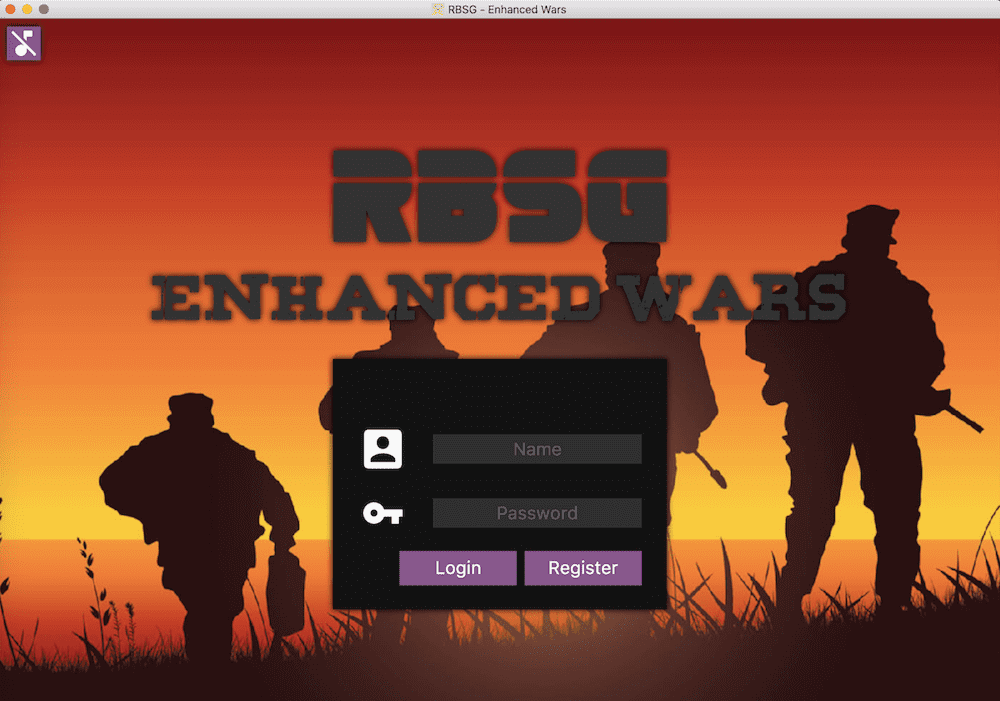
\includegraphics[width=0.8\textwidth]{images/old_state/login/Login.png}
    				\caption{Release \RN{2}: Login Szene}
    				\label{Login}
			    \end{figure}
			    \ \\ Versuchte der Nutzer sich anzumelden oder zu registrieren, erschien ein Lade-Indikator (siehe Abbildung \ref{Login_Form}) und die Buttons und Textfelder wurden deaktiviert. Machte der Nutzer dabei einen Fehler, oder konnte keine Verbindung zum Server hergestellt werden, erschien eine Fehlermeldung (siehe Abbildung \ref{Login_Form}). Der Login war internationalisiert und der Untertitel \glqq Enhanced Wars\grqq\ war animiert. Weiterhin konnte der Nutzer die Musik "uber den Musik Button in der Ecke ein- und ausschalten. \\
			    \begin{figure}[H]
                    \centering
                    \begin{subfigure}[h]{0.3\linewidth}
                        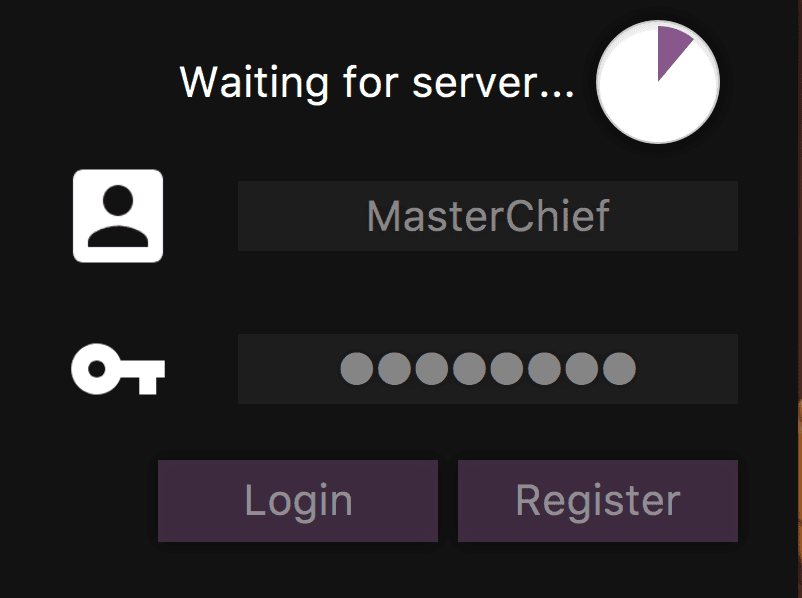
\includegraphics[width=\linewidth]{images/old_state/login/Indicator.png}
                        \caption{Indikator}
                    \end{subfigure}
                    \begin{subfigure}[h]{0.3\linewidth}
                        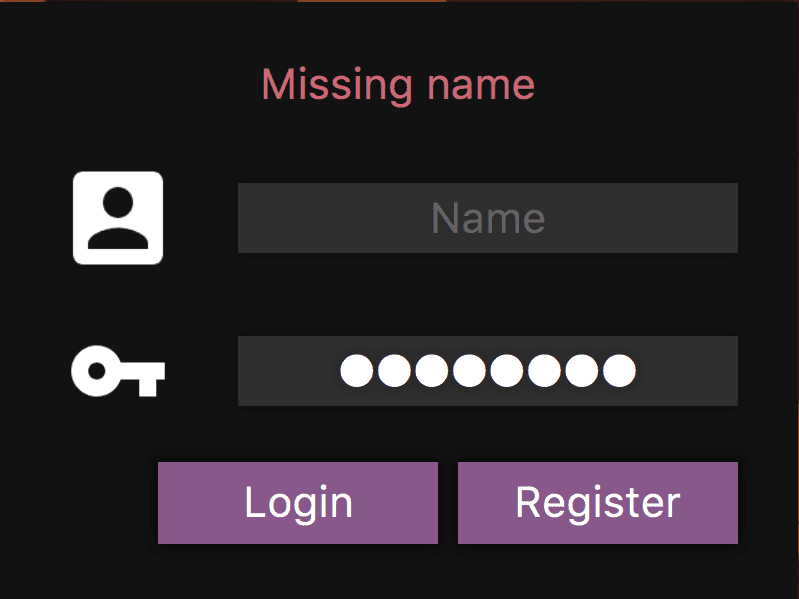
\includegraphics[width=\linewidth]{images/old_state/login/MissingName.png}
                        \caption{Missing Name}
                    \end{subfigure}
                    \begin{subfigure}[h]{0.3\linewidth}
                        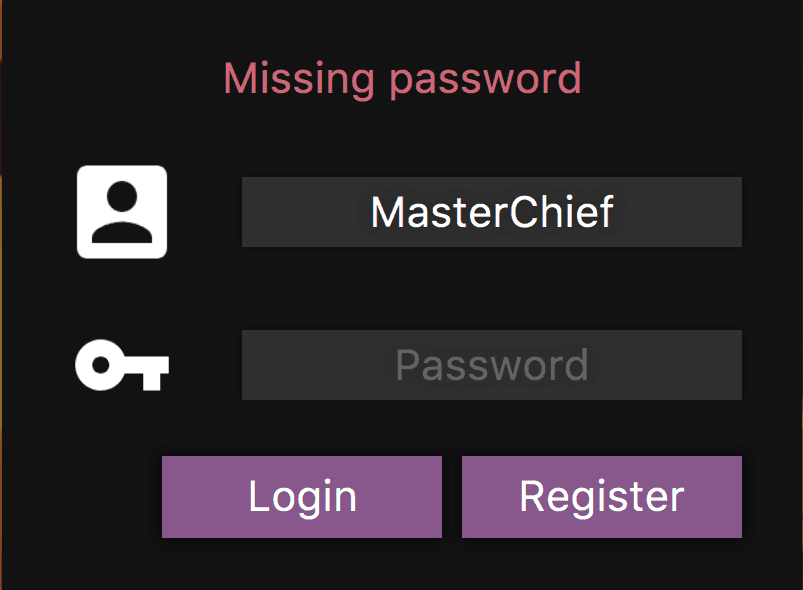
\includegraphics[width=\linewidth]{images/old_state/login/MissingPassword.png}
                        \caption{Missing Password}
                    \end{subfigure}
                    \begin{subfigure}[h]{0.3\linewidth}
                        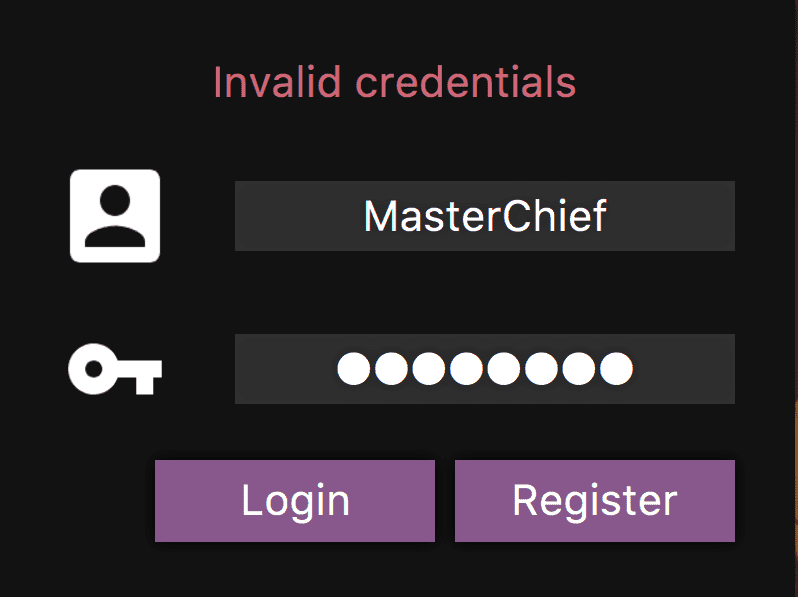
\includegraphics[width=\linewidth]{images/old_state/login/InvalidCredentials.png}
                        \caption{Invalid Credentials}
                    \end{subfigure}
                    \begin{subfigure}[h]{0.3\linewidth}
                        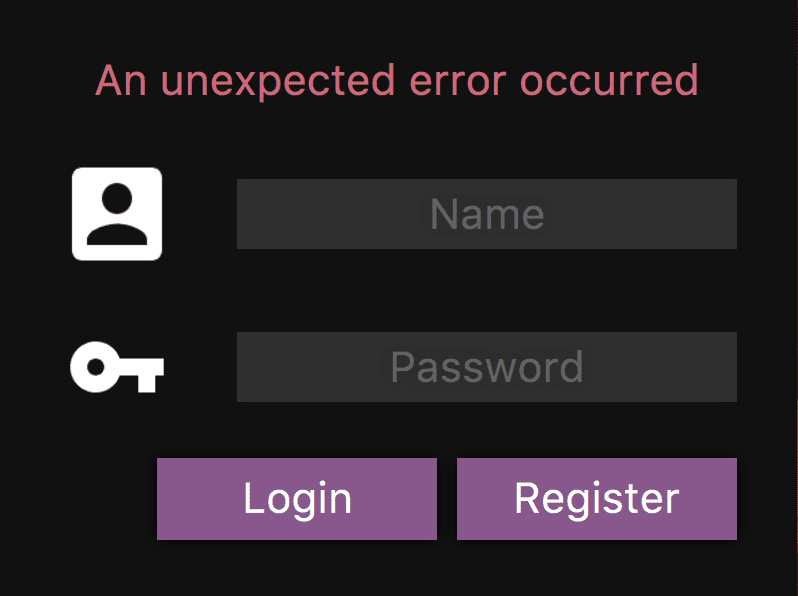
\includegraphics[width=\linewidth]{images/old_state/login/UnexpectedError.png}
                        \caption{Unexpected Error}
                    \end{subfigure}
                    \caption{Release \RN{2}: Login Formular}
                    \label{Login_Form}
                \end{figure}
            \subsubsection{Lobby} \label{LOBBY}
                Die Lobby zeigte eine Liste von allen Spielern, welche sich ebenfalls in der Lobby befanden, und allen Spielen an. Diese Listen aktualisierten sich, wenn der Server eine entsprechende Nachricht schickte. Der Nutzer konnte sich "uber die Buttons oben rechts ausloggen, die Sprache "andern oder die Musik an- und ausschalten. Der Chat wurde unten links angezeigt. Rechts sah der Nutzer eine Liste mit allen vollst"andigen Armeen. Hatte der Nutzer keine vollst"andige Armee ausgew"ahlt, konnte er kein Spiel erstellen (siehe Abbildung \ref{Lobby_No_Army_Selected}) und auch keinem Spiel beitreten. \\
                \begin{figure}[H] 
    				\centering
    				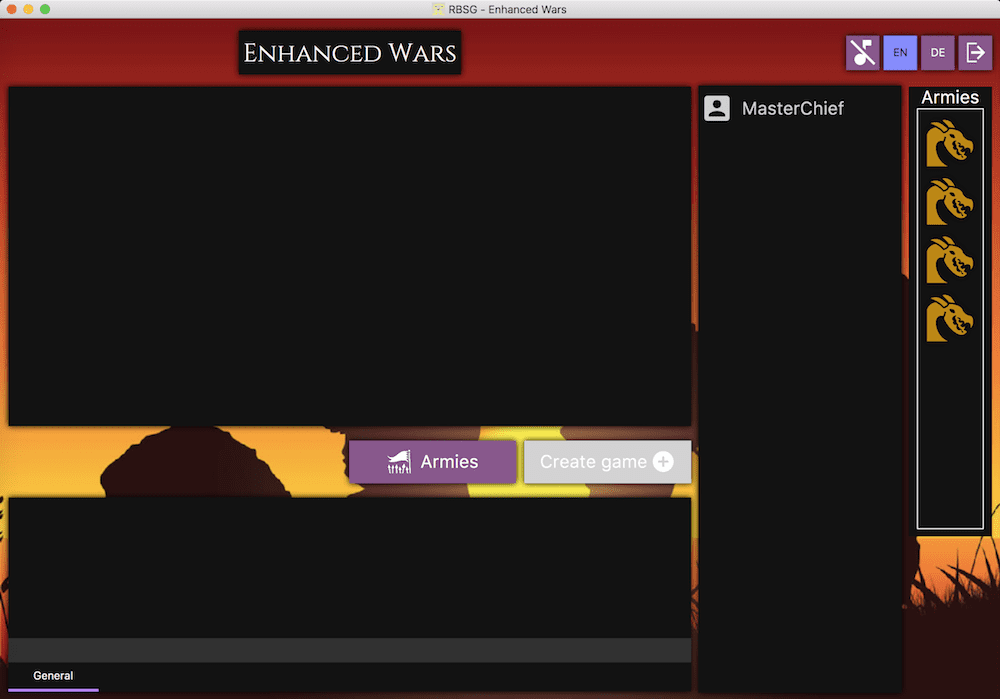
\includegraphics[width=0.8\textwidth]{images/old_state/lobby/NoArmySelected.png}
    				\caption{Release \RN{2}: Lobby Szene: Keine Armee ausgew"ahlt}
    				\label{Lobby_No_Army_Selected}
			    \end{figure}
			    \begin{wrapfigure}[9]{r}{0.35\textwidth}
                    \begin{center}
                        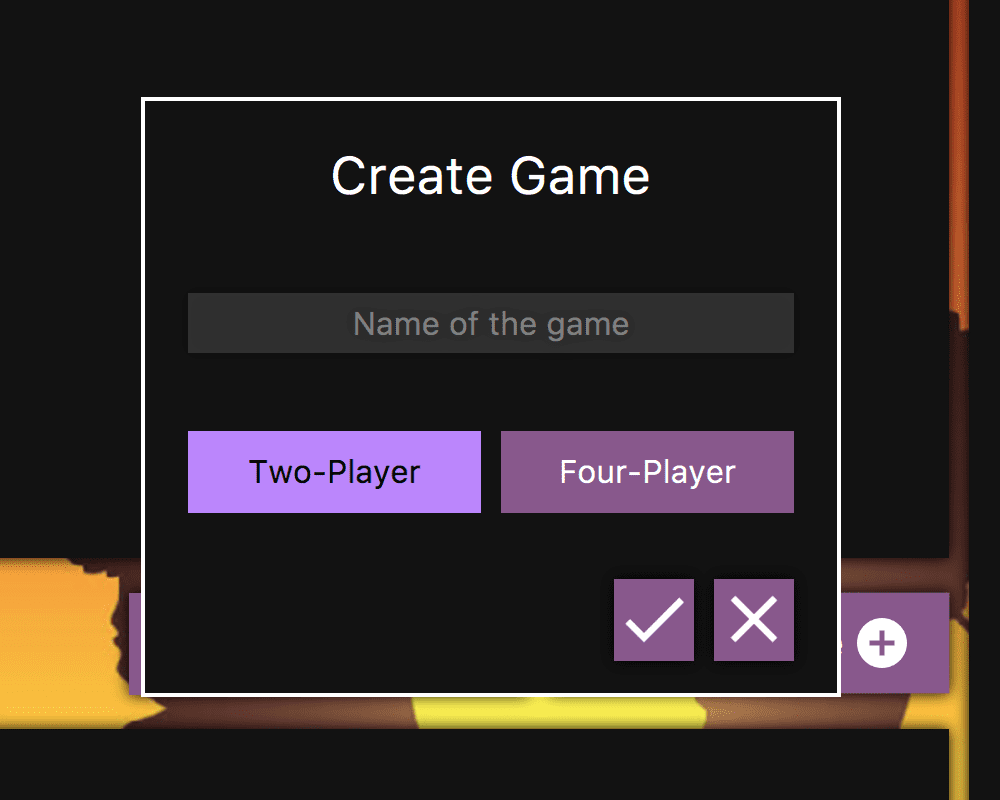
\includegraphics[width=0.35\textwidth]{images/old_state/lobby/CreateGame.png}
                    \end{center}
                    \caption{Release \RN{2}: Create Game Formular}
                    \label{Create_Game}
                \end{wrapfigure}
			    \ \vspace{0.5cm} \\ Hatte der Nutzer aber eine Armee ausgew"ahlt, konnte er ein Spiel erstellen oder einem Spiel beitreten (siehe Abbildung \ref{Create_Game} oder \ref{Lobby_Language}). Spiel erstellen funktionierte "uber den Create Game Button (siehe Abbildung \ref{Lobby_Army_Selected}). Der Nutzer hatte die Auswahl zwischen einem 2-Spieler-Spiel und einem 4-Spieler-Spiel. Erstellte er ein Spiel trat er diesem automatisch bei. Die Lobby war auch internationalisiert (vgl. Abbildung \ref{Lobby_Army_Selected} mit \ref{Lobby_Language}). \\
			    \begin{figure}[H] 
    				\centering
    				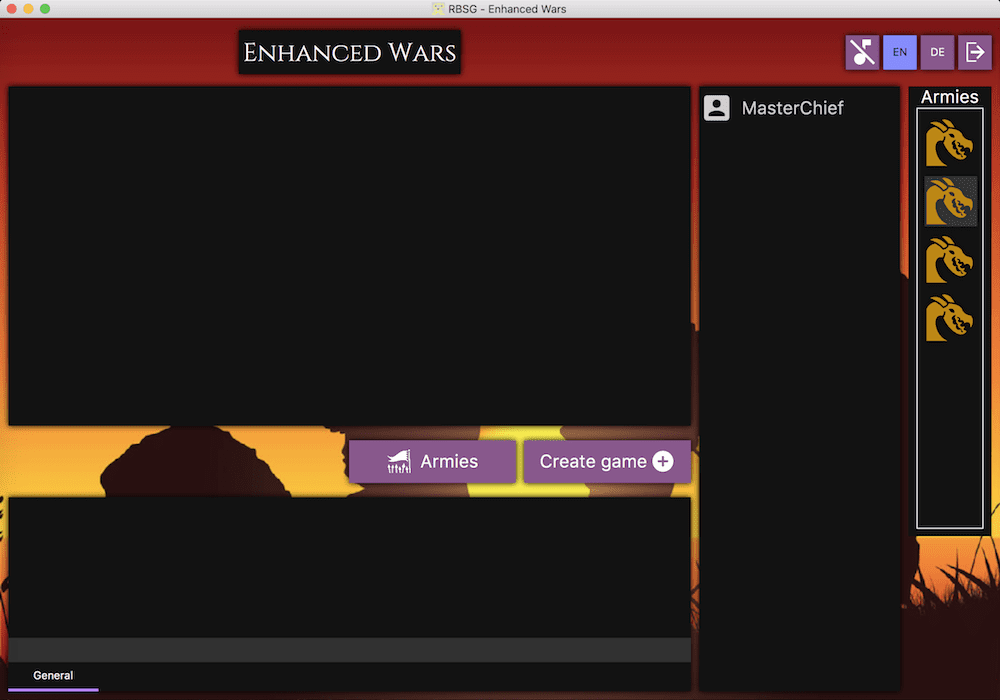
\includegraphics[width=0.8\textwidth]{images/old_state/lobby/ArmySelected.png}
    				\caption{Release \RN{2}: Lobby Szene: Armee ausgew"ahlt}
    				\label{Lobby_Army_Selected}
			    \end{figure}
			    \begin{figure}[H] 
    				\centering
    				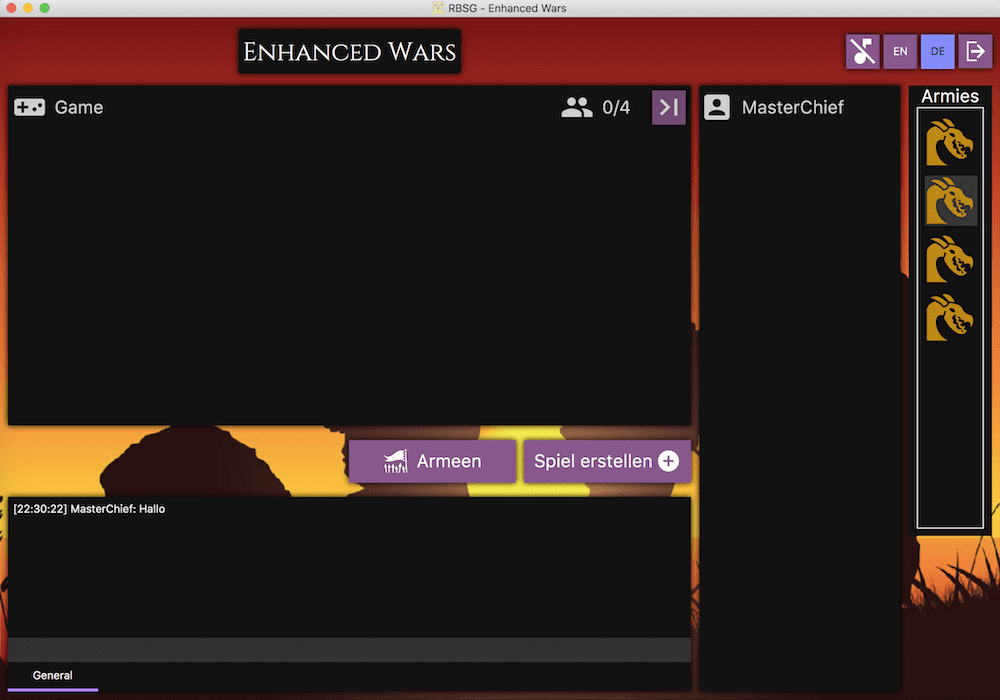
\includegraphics[width=0.8\textwidth]{images/old_state/lobby/International+Chat+GameCreated.png}
    				\caption{Release \RN{2}: Lobby Szene: Sprache DE}
    				\label{Lobby_Language}
			    \end{figure}
		    \subsubsection{Army Manager}
		        Im Army Manager gab es eine Liste der Einheiten, die der Nutzer w"ahlen konnte, und eine Liste der Einheiten, die sich der aktuell ausgew"ahlten Armee befanden. In der Mitte stand der Name der ausgew"ahlten Armee, ein Plus (+) und ein Minus (-) Button, um Einheiten der Armee hinzuzuf"ugen oder um sie zu entfernen und ein Z"ahler, der anzeigte, wie viele Einheiten bereits in der Armee waren. Neben der Einheitenliste war eine Vorschau der aktuell ausgew"ahlten Einheit. Neben diesem Feld wurden die Eigenschaften der Einheit angezeigt und welche Einheitentypen die ausgew"ahlte Einheit angreifen konnte. War keine Einheit ausgew\"ahlt wurden Platzhalter angezeigt (siehe Abbildung \ref{Army_Manager_No_Unit_Selected}), ansonsten Zahlenwerte (siehe Abbildung \ref{Army_Manager_Unit_Selected}). \\
		        \begin{figure}[H] 
    				\centering
    				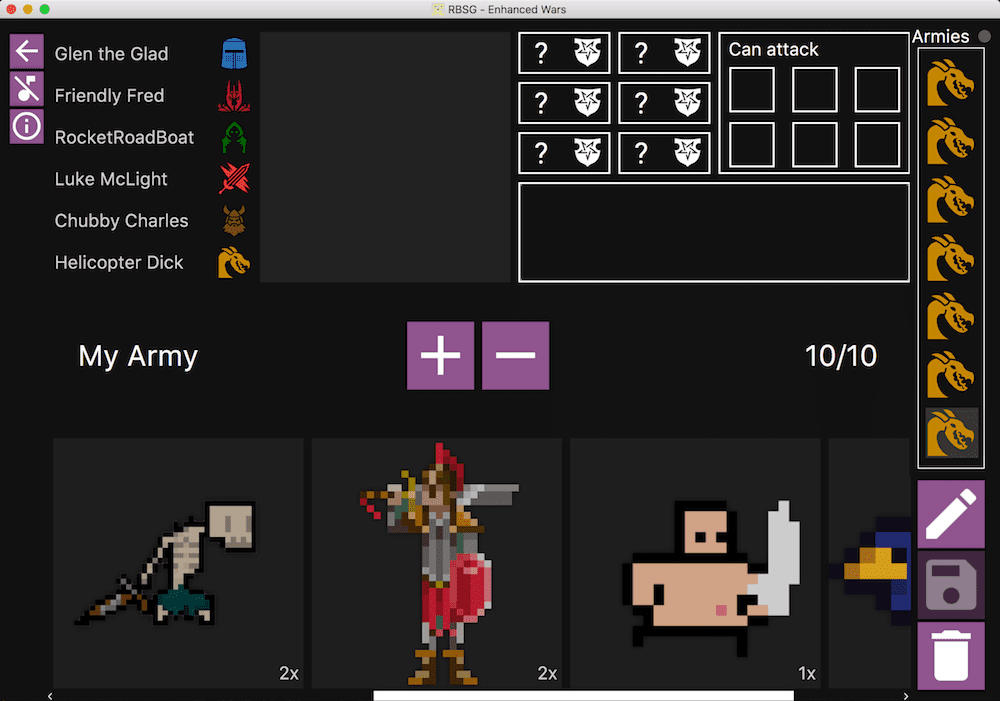
\includegraphics[width=0.8\textwidth]{images/old_state/army_manager/NoUnitSelected.png}
    				\caption{Release \RN{2}: Army Manager Szene: Keine Einheit ausgew"ahlt}
    				\label{Army_Manager_No_Unit_Selected}
			    \end{figure}
			    \begin{figure}[H] 
    				\centering
    				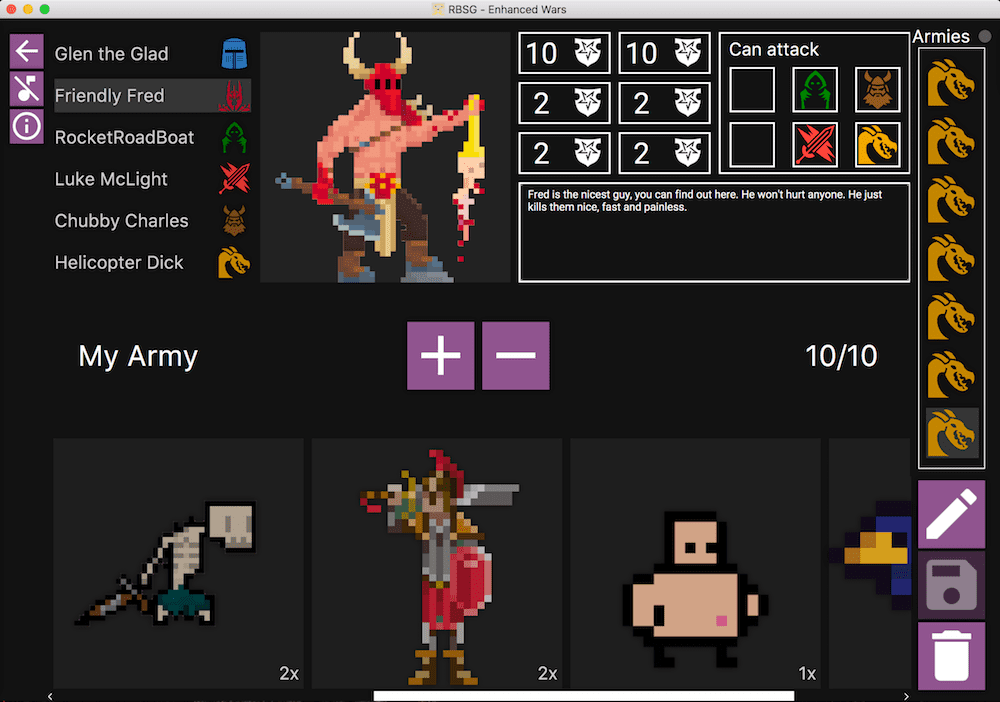
\includegraphics[width=0.8\textwidth]{images/old_state/army_manager/UnitSelected.png}
    				\caption{Release \RN{2}: Army Manager Szene: Einheit ausgew"ahlt}
    				\label{Army_Manager_Unit_Selected}
			    \end{figure}
			    \ \\ Darunter befand sich der Lore Text der ausgew"ahlten Einheit. Oben links befanden sich Buttons zum Verlassen des ArmyBuilders, zum Ein- oder Ausschalten der Musik, sowie zum Anzeigen eines Overlays, welches die Eigenschaften der Einheiten erkl"arte (siehe Abbildung \ref{Property_Infoo}). Unten rechts befanden sich Buttons zum L\"oschen und Speichern von Armeen. \\
			    \begin{figure}[H]
                    \centering
                    \begin{minipage}{0.5\textwidth}
                        \centering
                        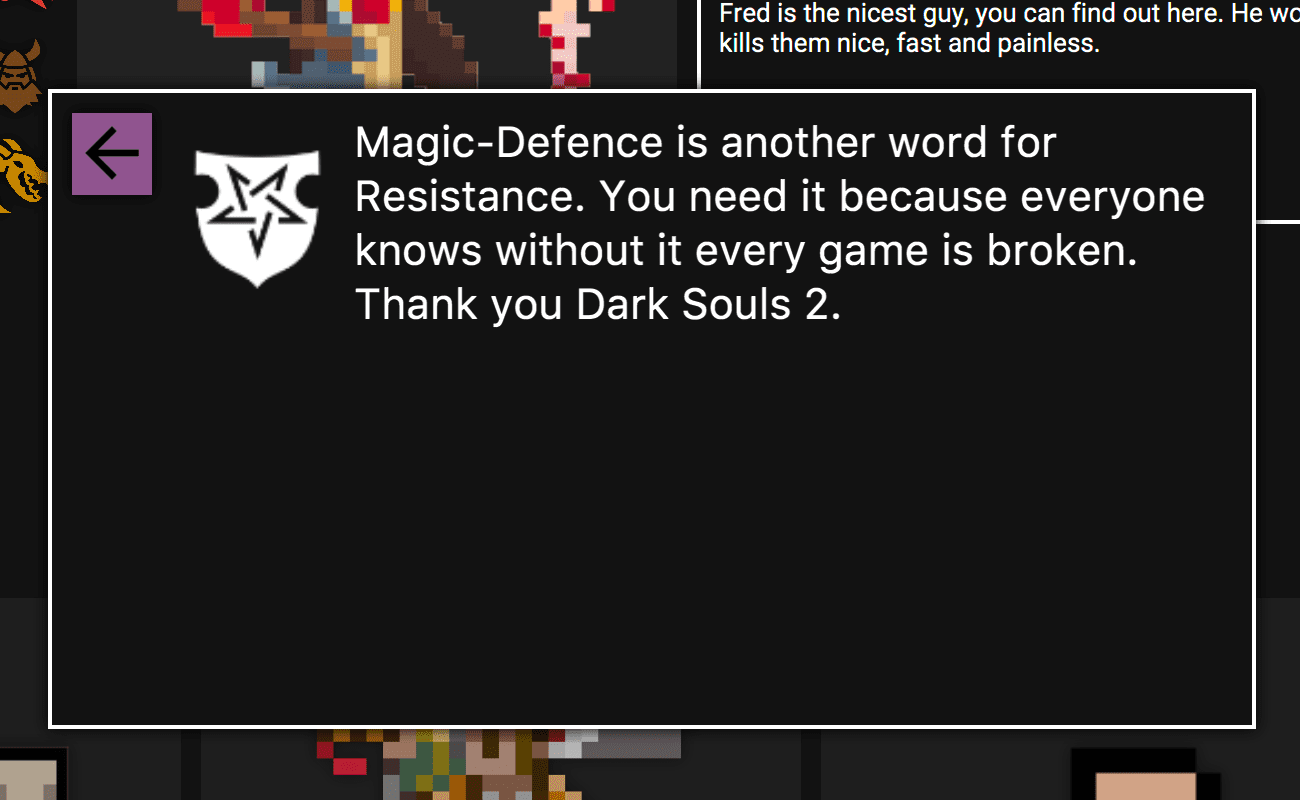
\includegraphics[width=0.8\textwidth]{images/old_state/army_manager/PropertyInfo.png}
                        \caption{Release \RN{2}: Property Info}
                        \label{Property_Infoo}
                    \end{minipage}%
                    \begin{minipage}{0.5\textwidth}
                        \centering
                        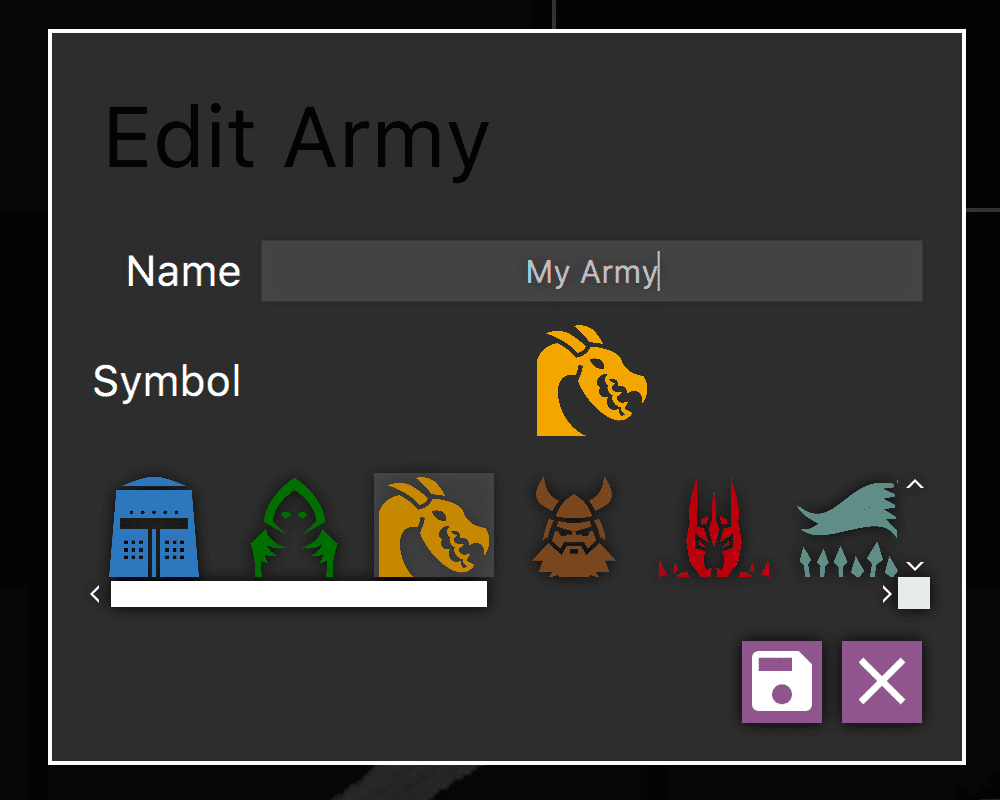
\includegraphics[width=0.8\textwidth]{images/old_state/army_manager/EditArmy.png}
                        \caption{Release \RN{2}: Armee bearbeiten}
                        \label{Edit_Army}
                    \end{minipage}
                \end{figure}
                \ \\ Der Speichern Button blieb deaktiviert (siehe Abbildung \ref{Army_Manager_No_Unit_Selected}) bis die Armee ver\"andert wurde (siehe Abbildung \ref{Army_Manager_Ready_To_Save}). Ein weiterer Button erm\"oglichte das "Andern des Armeenamens oder -icons. Dazu "offnete sich ein weiteres Overlay (siehe Abbildung \ref{Edit_Army}). \\
                \begin{figure}[H] 
    				\centering
    				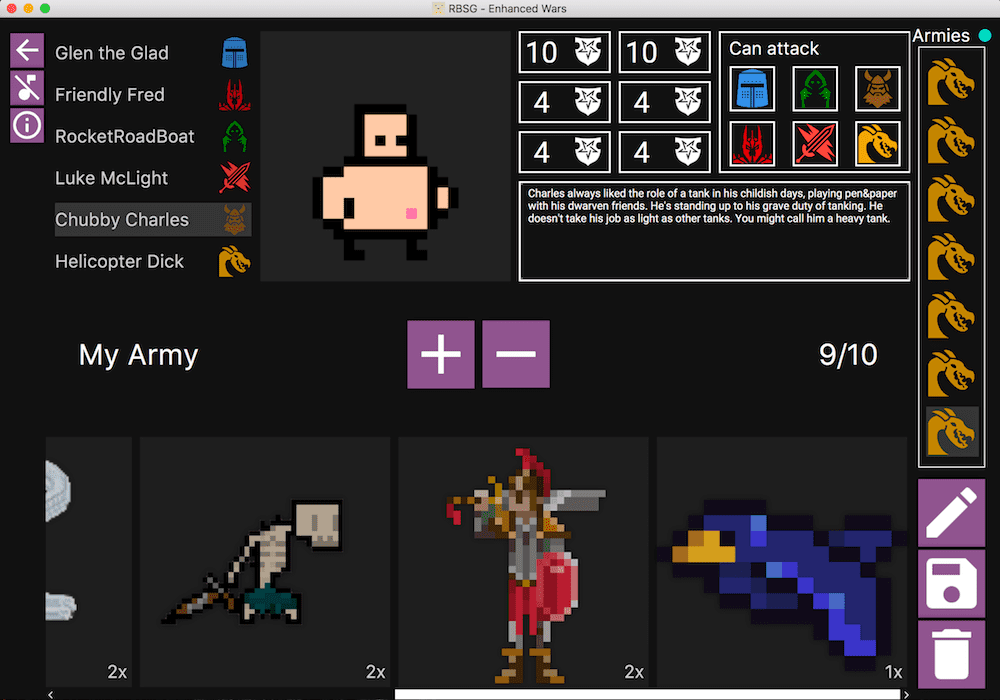
\includegraphics[width=0.8\textwidth]{images/old_state/army_manager/ArmyReadyToSave.png}
    				\caption{Release \RN{2}: Army Manager Szene: Speicherbar}
    				\label{Army_Manager_Ready_To_Save}
			    \end{figure}
	        \subsubsection{Warteraum} \label{WAITING_ROOM}
                Trat der Nutzer dem Warteraum bei sah er oben rechts verschiedene Buttons zum Verlassen des Spiels, zum Ein- und Ausschalten der Musik und zum Anzeigen von Informationen. \\
                \begin{figure}[H] 
    				\centering
    				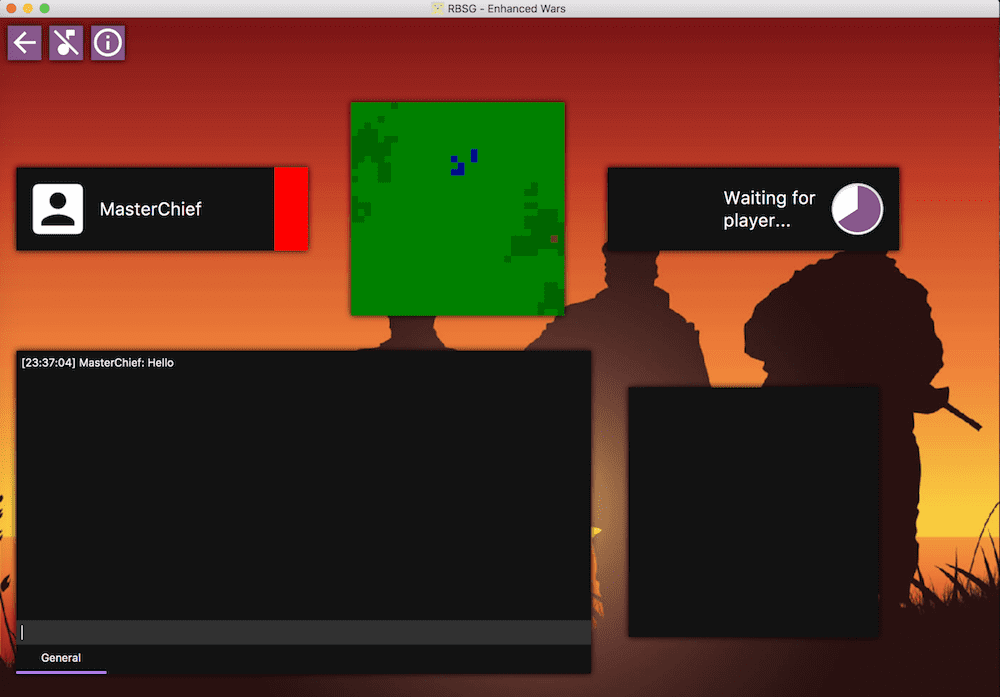
\includegraphics[width=0.8\textwidth]{images/old_state/waiting_room/2Player.png}
    				\caption{Release \RN{2}: Warteraumszene: 2 Spieler}
    				\label{Waiting_Room_2}
			    \end{figure}
			    \begin{figure}[H] 
    				\centering
    				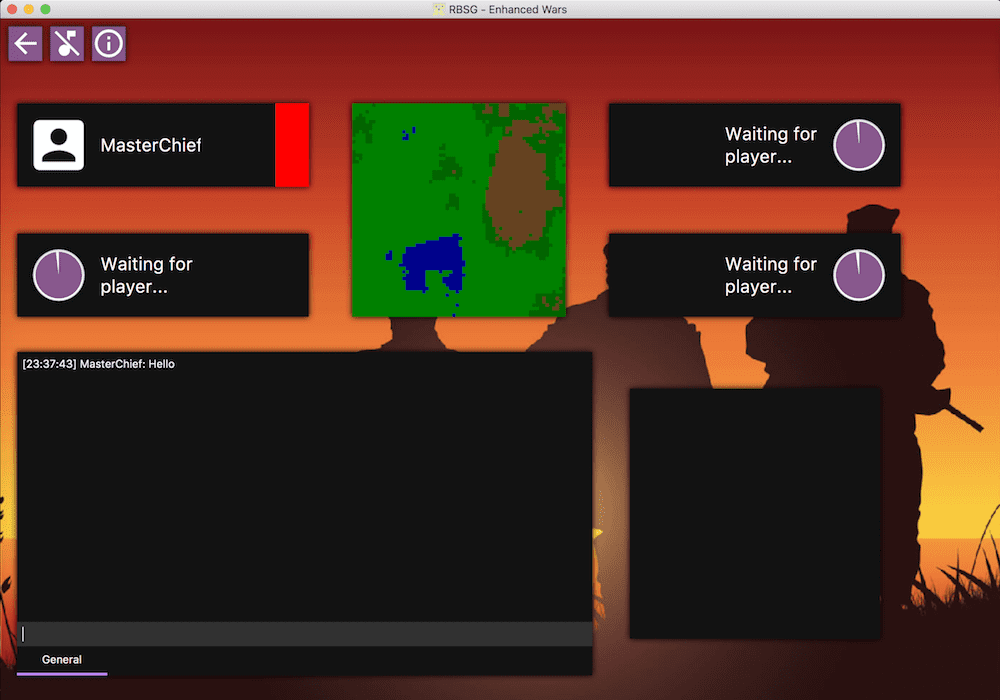
\includegraphics[width=0.8\textwidth]{images/old_state/waiting_room/4Player.png}
    				\caption{Release \RN{2}: Warteraumszene: 4 Spieler}
    				\label{Waiting_Room_4}
			    \end{figure}
			    \ \\  Da dieser Button noch keine spezielle Funktion hatte, wechselte der Nutzer mit diesem testweise zum Spielfeld. Oben in der Mitte wurde die Kartenvorschau angezeigt.  Links und rechts daneben waren die Spielerkarten zu sehen. Je nachdem ob der Nutzer ein 2-Spieler-Spiel oder ein 4-Spieler-Spiel startete, befanden sich dort zwei oder vier Spielerkarten (siehe Abbildung \ref{Waiting_Room_2} und \ref{Waiting_Room_4}). Auf den Spielerkarten befanden sich der Name und die Farbe des jeweiligen Spielers. Waren noch nicht genug Spieler dem Spiel beigetreten, wurden Lade-Indikatoren in den Spielerkarten angezeigt. Darunter war der Chat und daneben eine freies Feld f"ur ein Minispiel, welches noch implementiert werden sollte.
	        \subsubsection{Ingame}
	            Die Spielszene zeigte bisher nur die Karte und das initiale Spielgeschehen. Die initialen Einheiten wurden ebenfalls angezeigt. Weiterhin gab es einen Button zum Verlassen des Spiels. Zwei weitere Buttons kontrollierten das Zoomen auf dem Spielfeld (siehe Abbildung \ref{Ingame}, \ref{Ingame_In} und \ref{Ingame_Out}). \\
	            \begin{figure}[H] 
    				\centering
    				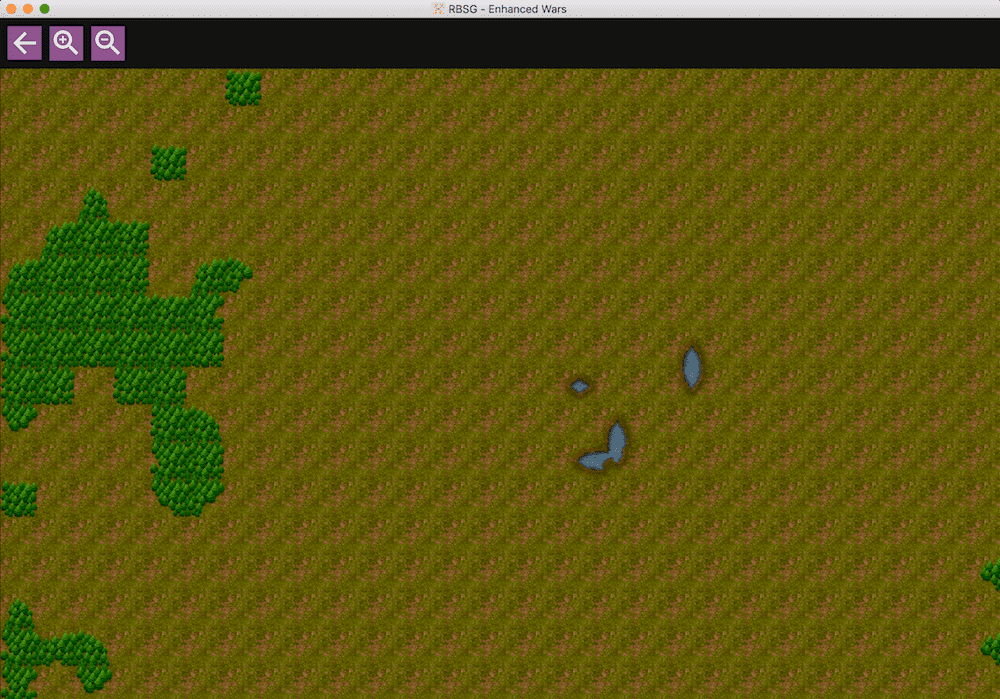
\includegraphics[width=0.8\textwidth]{images/old_state/ingame/Ingame.png}
    				\caption{Release \RN{2}: Spielszene}
    				\label{Ingame}
			    \end{figure}
			    \begin{figure}[H] 
    				\centering
    				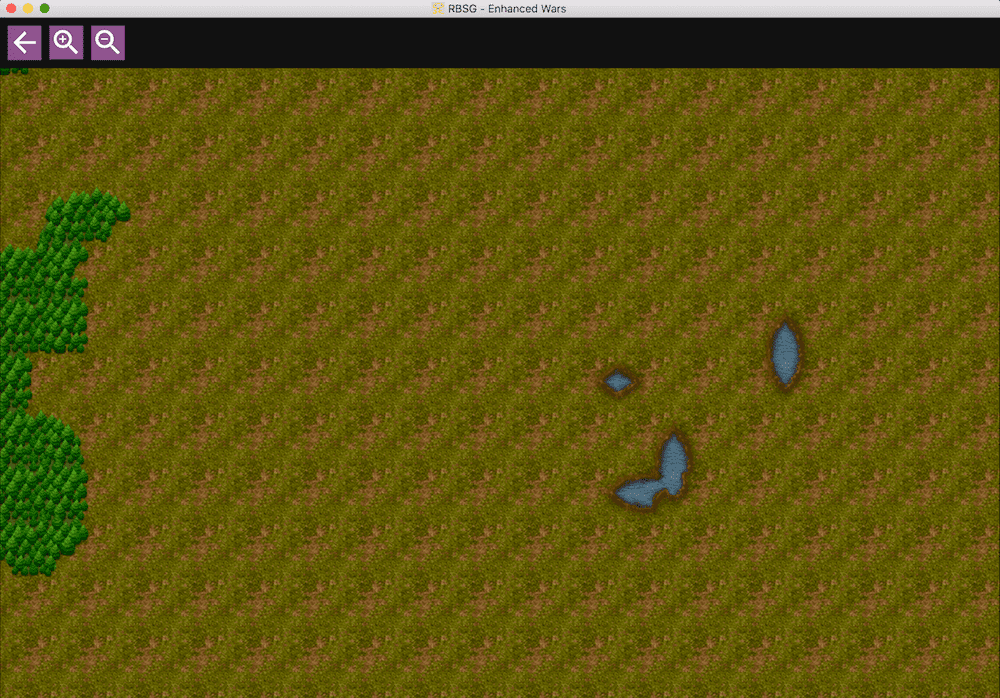
\includegraphics[width=0.8\textwidth]{images/old_state/ingame/ZoomIn.png}
    				\caption{Release \RN{2}: Spielszene: Zoom In}
    				\label{Ingame_In}
			    \end{figure}
			    \begin{figure}[H] 
    				\centering
    				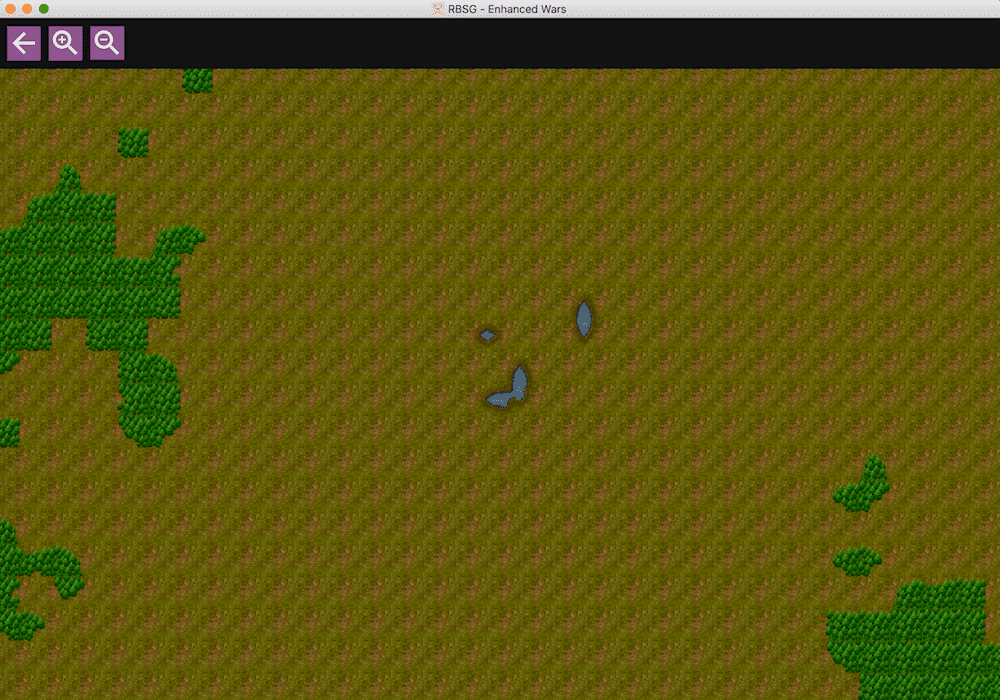
\includegraphics[width=0.8\textwidth]{images/old_state/ingame/ZoomOut.png}
    				\caption{Release \RN{2}: Spielszene: Zoom Out}
    				\label{Ingame_Out}
			    \end{figure}
	\newpage
		    \subsubsection{Weitere Features}
		        \begin{wrapfigure}[23]{r}{0.35\textwidth}
                    \begin{center}
                        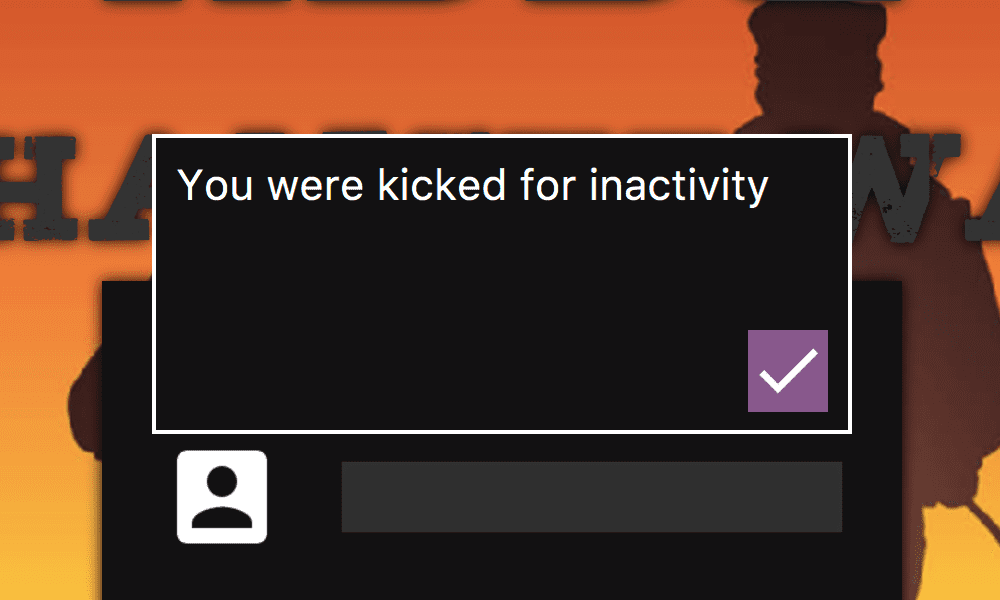
\includegraphics[width=0.35\textwidth]{images/old_state/additional/LoginFailure.png}
                        \caption{Release \RN{2}: Login Fehler}
                        \label{Login_Failure}
                    \end{center}
                    \begin{center}
                        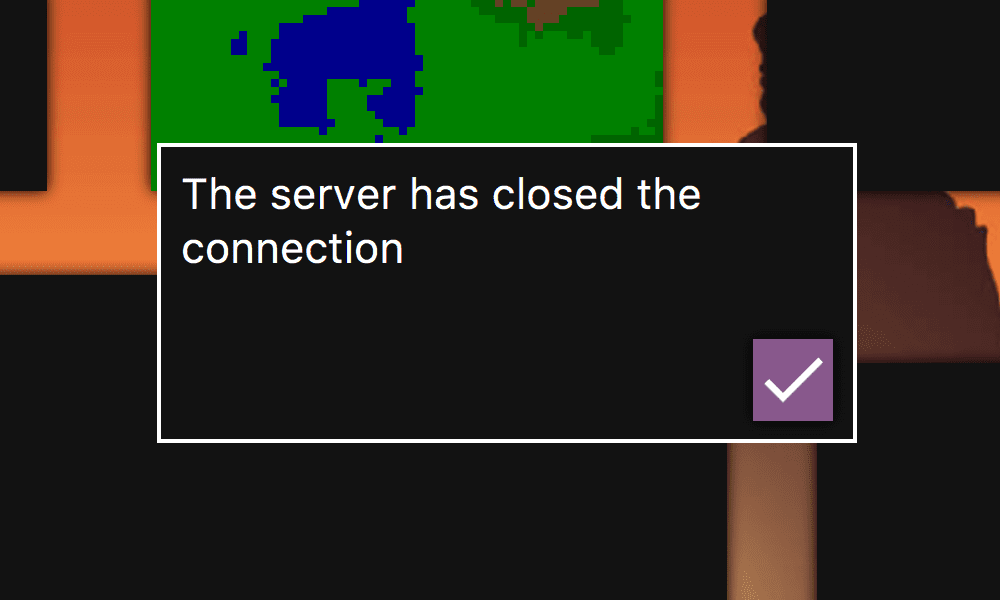
\includegraphics[width=0.35\textwidth]{images/old_state/additional/WaitingRoomFailure.png}
                        \caption{Release \RN{2}: Spielfehler}
                        \label{Game_Failure}
                    \end{center}
                \end{wrapfigure}
		        \ \\ Weiterhin wurde seit den ersten beiden Releases ein Dark Theme Styling implementiert, wie auf allen vorangegangenen Abbildungen zu sehen war. Musik und Internationalisierung waren zwar optional, aber funktionierten in jeder Szene. Der Nutzer konnte auch nach Belieben Chuck Norris Zitate "uber den Chatbefehl \glqq /chuckMe\grqq\ im Chat versenden. Chatnachrichten wurden zudem mit einem Zeitstempel versehen. Wenn der Nutzer eine private Nachricht in einem nicht aktiven Tab erhielt, wurde dieser mit einem farbigen Punkt markiert. Die Kartenvorschau im Warteraum, das Zoomen im Spiel, das \"Andern der Armeenamen und -icons waren optional. Der Autojoin nach Erstellen eines Spiels war ebenfalls optional. Ein weiteres Feature war, dass der Client dem Nutzer Fehlermeldungen (siehe Abbildung \ref{Login_Failure} und \ref{Game_Failure}) zeigte, wenn der Server die Verbindung unerwartet schloss. Der Nutzer wurde je nach Fehler in den Login oder die Lobby zur"uckgeschickt. Au{\ss}erdem gab es ein Fenster, in dem sich der Nutzer noch einmal entscheiden konnte, ob er sich wirklich ausloggen oder das Spiel verlassen m"ochte (siehe Abbildung \ref{Leave_Game} und \ref{Logout}). \\
		        \begin{figure}[H]
                    \centering
                    \begin{minipage}{0.55\textwidth}
                        \centering
                        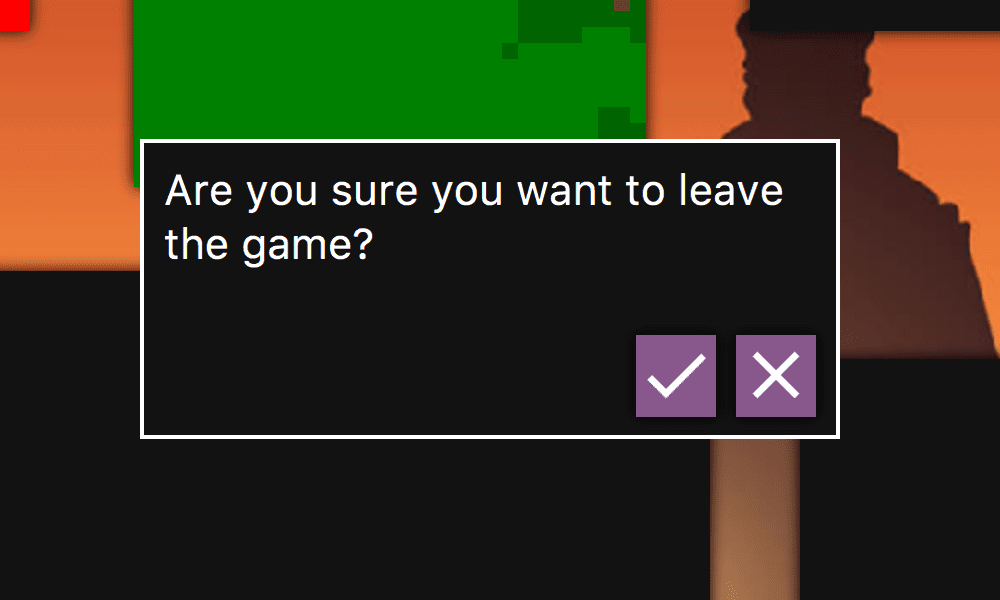
\includegraphics[width=0.55\textwidth]{images/old_state/additional/LeaveGame.png}
                        \caption{Release \RN{2}: Spiel verlassen}
                        \label{Leave_Game}
                    \end{minipage}%
                    \begin{minipage}{0.55\textwidth}
                        \centering
                        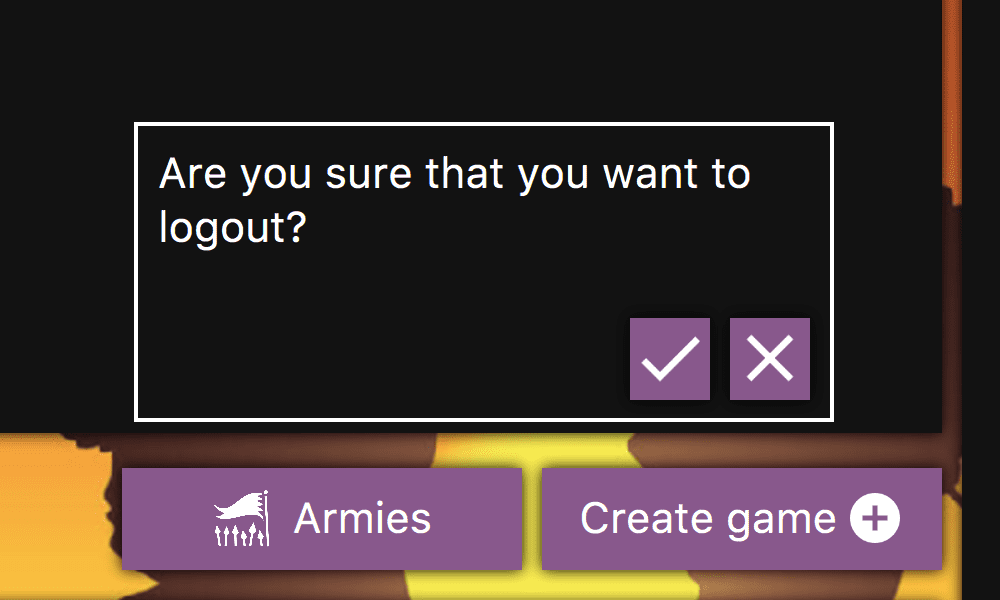
\includegraphics[width=0.55\textwidth]{images/old_state/additional/Logout.png}
                        \caption{Release \RN{2}: Logout}
                        \label{Logout}
                    \end{minipage}
                \end{figure}
                \ \\ Die C0 Testabdeckung betrug zum Ende des Releases \RN{2} 77\%.
                \begin{figure}[H] 
    				\centering
    				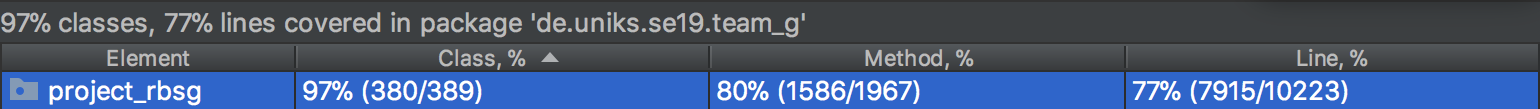
\includegraphics[width=\textwidth]{images/old_state/Coverage.png}
    				\caption{Release \RN{2}: C0 Testabdeckung (Siehe Line, \%)}
    				\label{Coverage}
			    \end{figure}
    \newpage
	    \subsection{Mockups}
	        Aufgrund der Releaseanforderungen wurden f"ur das Kundentreffen am 1.7.2019 Mockups zu der neuen Spielszene erstellt. Weiterhin gab es Mockups zur Lobby und zum Warteraum. Diese wurden nach dem Erscheinen der Serverdokumentation noch erweitert. Im sechsten Sprint wurden die Mockups noch einmal angepasst, da sich grundlegende \"Anderungen ergaben. Das Kontextmen"u wurde durch die Sidebar ersetzt. Die Mockups waren im Stil des Dark Theme und sollten an die UI aus den vorherigen Releases ankn"upfen.
	        \subsubsection{Lobby}
	           Es wurde gefordert, in der Lobby ein Button hinzuzuf"ugen, der es dem Nutzer erlaubte, einem Beobachtungsmodus beizutreten. Des Weiteren sollte die Armeeauswahl aus der Lobby entfernt werden und in den Warteraum verlegt werden. \\
	            \begin{figure}[H] 
    				\centering
    				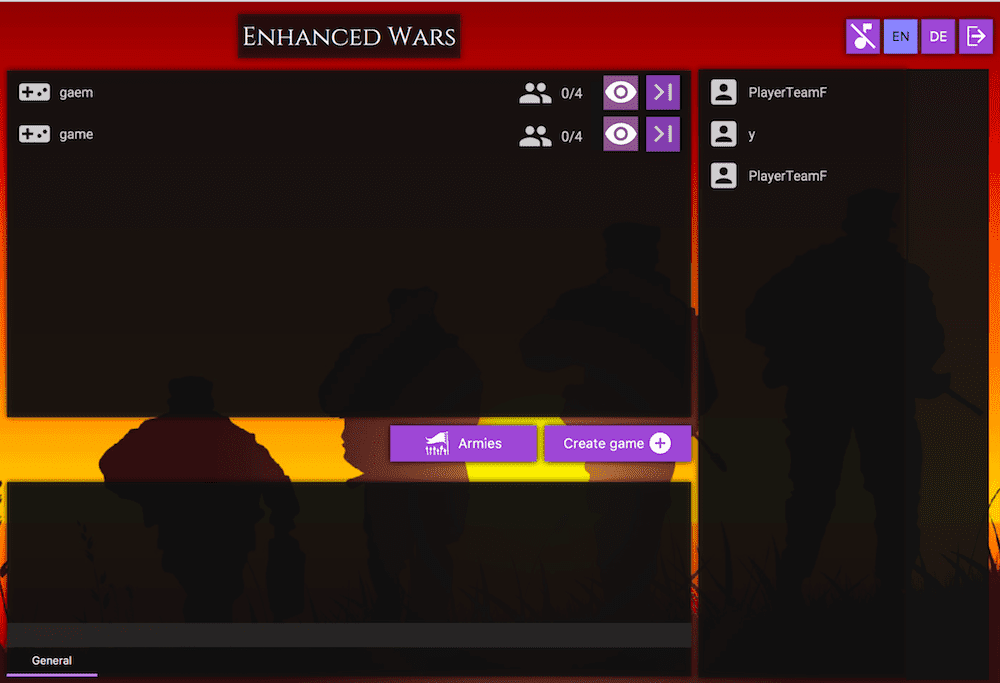
\includegraphics[width=0.8\textwidth]{images/mockups/LobbyWatchMode.png}
    				\caption{Mockup: Beobachtungsmodus Lobby}
    				\label{Watch_Mode}
			    \end{figure}
		    \subsubsection{Warteraum}
		        Da der Warteraum im Release \RN{2} (siehe Kapitel \ref{WAITING_ROOM}) schon gr"o"stenteils vorhanden war, musste nur noch das Setzen von Spielern als bereit hinzugef"ugt werden. Dies sollte passieren, wenn der Nuzter eine Armee ausw"ahlte (siehe Abbildung \ref{Ready}). Die Armeeauswahl musste deswegen von der Lobby in den Warteraum umgezogen werden. Spielerkarten von bereiten Spielern solltenfarblich hervorgehoben werden und die Icons sollten sich schwarz f"arben. Wenn alle Spieler bereit waren, sollte ein Overlay angezeigt werden, in dem ein Indikator lud, bis zur Spielszene gewechselt wurde (siehe Abbildung \ref{Game_Start}). Auf den Mockups waren auch zwei optionale Features, das TicTacToe Spiel unten rechts und der Spielname in der Mitte des Spiels (siehe auf den Mockups mit Beispielnamen \glqq Enhanced Wars\grqq), zu sehen. \\
		        \begin{figure}[H] 
    				\centering
    				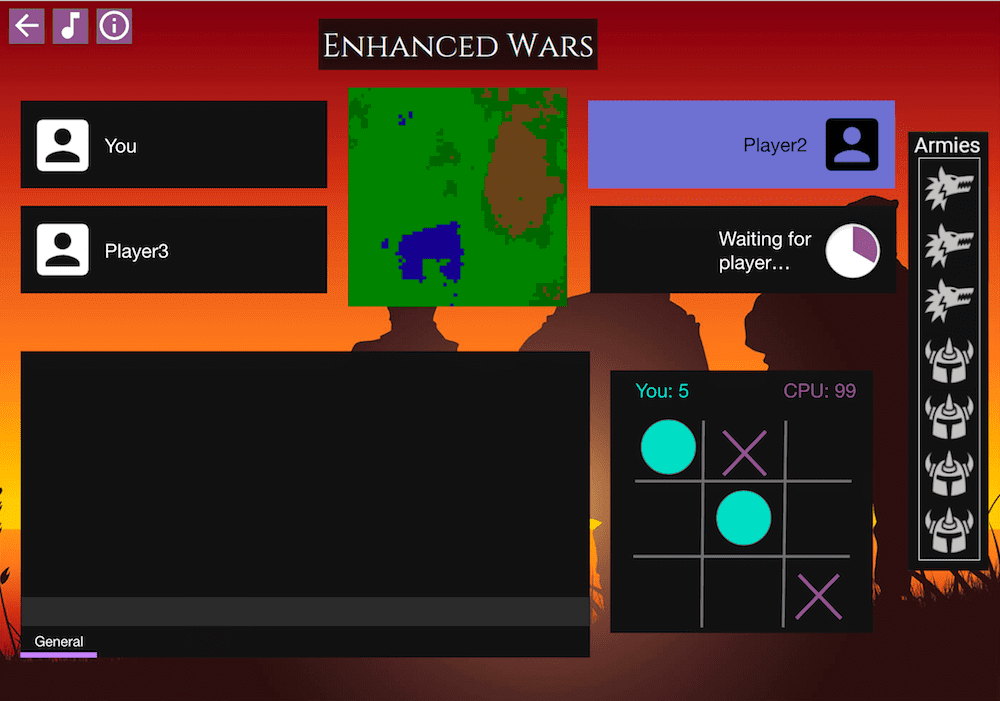
\includegraphics[width=0.8\textwidth]{images/mockups/NotReady.png}
    				\caption{Mockup: Nutzer nicht bereit}
    				\label{Not_Ready}
			    \end{figure}
			    \begin{figure}[H] 
    				\centering
    				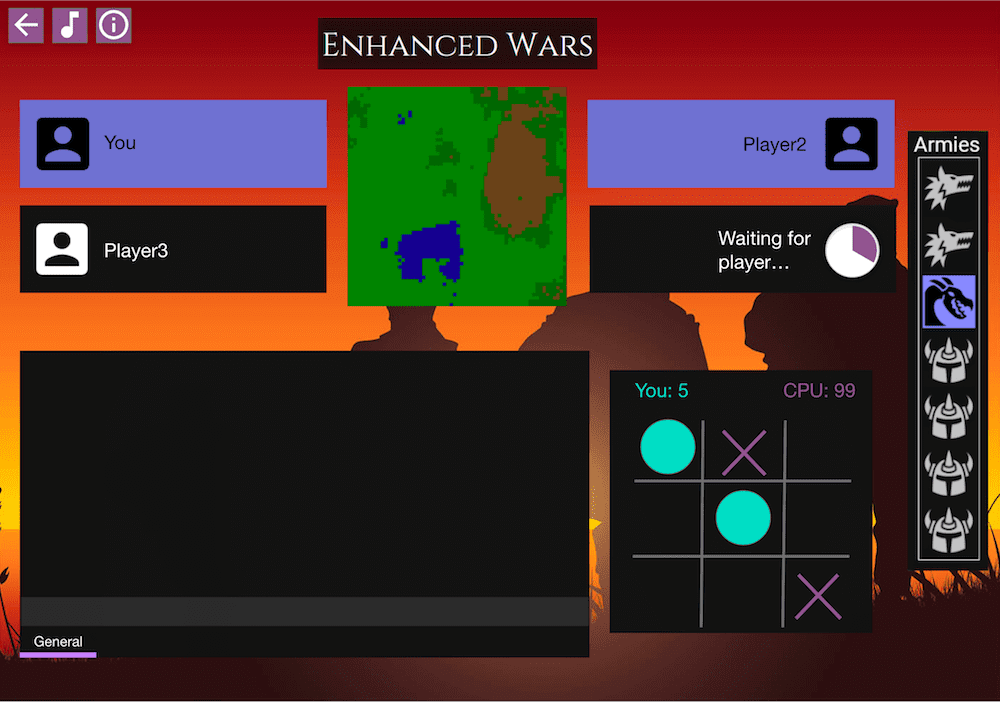
\includegraphics[width=0.8\textwidth]{images/mockups/Ready.png}
    				\caption{Mockup: Nutzer bereit}
    				\label{Ready}
			    \end{figure}
			    \begin{figure}[H] 
    				\centering
    				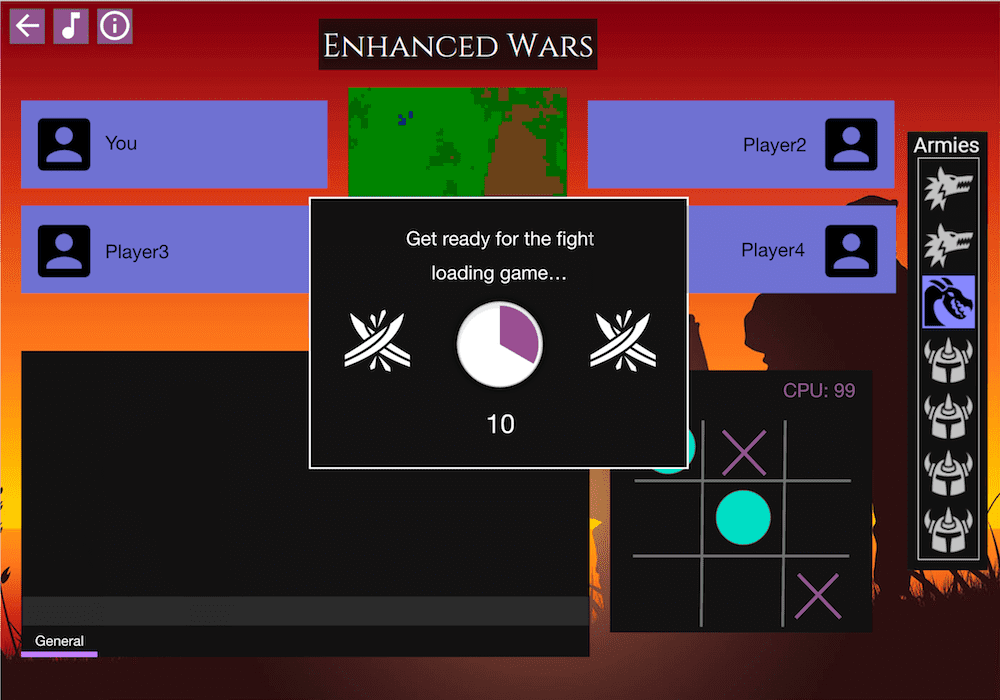
\includegraphics[width=0.8\textwidth]{images/mockups/StartGame.png}
    				\caption{Mockup: Spielstart}
    				\label{Game_Start}
			    \end{figure}
		    \subsubsection{Ingame}
		        Bisher zeigte die Spielszene nur das initiale Spielgeschehen. In diesem Release sollte diese Szene um den Chat, die Minikarte sowie die Spieler erweitert werden. \\
		        \begin{figure}[H] 
    				\centering
    				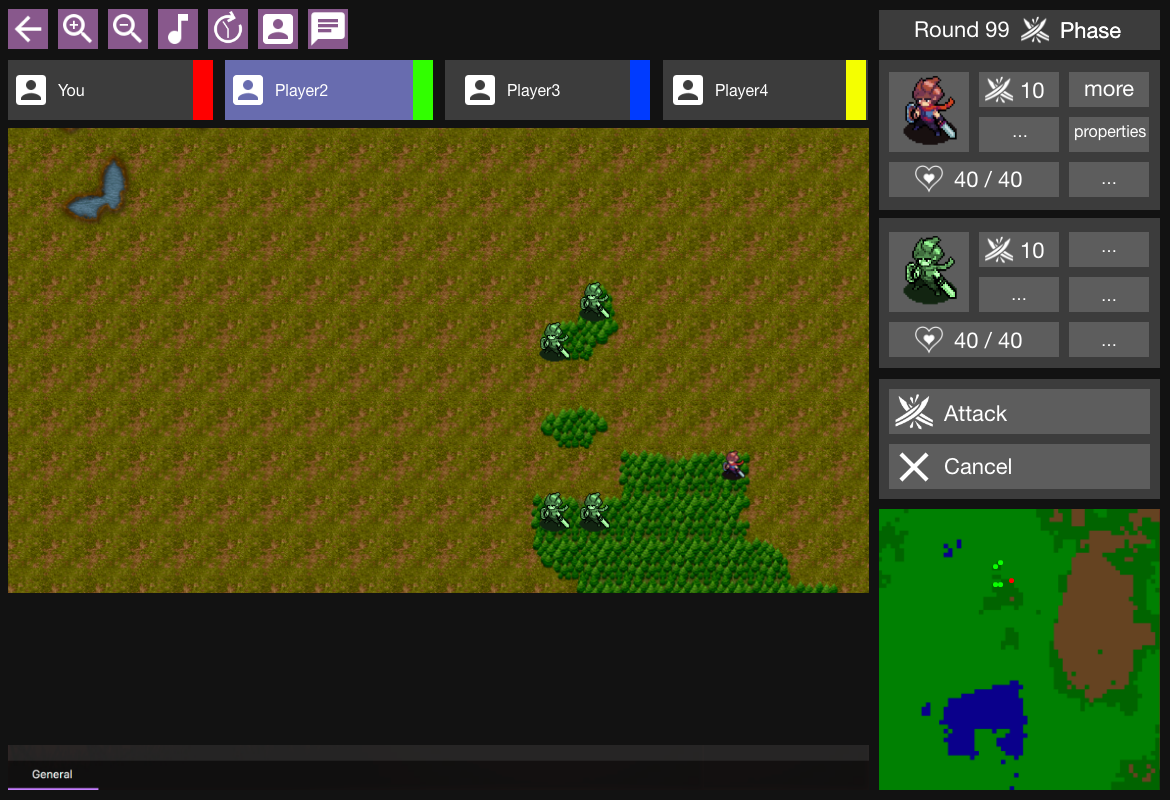
\includegraphics[width=0.8\textwidth]{images/mockups/Ingame.png}
    				\caption{Mockup: Ingame}
    				\label{Ingame_View}
			    \end{figure}
		    	\ \\   Der Chat und die Spielerkarten sollten auch "uber die jeweiligen Buttons oben in der Leiste eingeklappt werden k"onnen. Die Minikarte sollte unten rechts unter der Sidebar angezeigt werden. Die Sidebar befand sich rechts neben dem Spielfeld. Diese sollte die Einheiteninformationen und die Best"atigen und Abbrechen Buttons enthalten. Die aktuelle Runde und die aktuelle Phase sollten oben "uber der Sidebar angezeigt werden. Der aktuelle Spieler sollte in seiner Spielerkarte farblich hervorgehoben werden. In der oberen Leiste kam au"serdem der Musik Button zum Ein- und Ausschalten der Musik hinzu.
			    \subsubsubsection{Einheit ausw\"ahlen}
			        Der Server stellte drei Phasen zur Verf\"ugung, wenn ein Spieler an der Reihe war. Eine Bewegungsphase, in der mindestens eine Einheit bewegt werden musste, eine Angriffsphase, die \"ubersprungen werden konnte und eine Phase zum Verwenden der restlichen Bewegungspunktephase, die ebenfalls \"ubersprungen werden konnte. \\
			        \begin{figure}[H] 
    				    \centering
    				    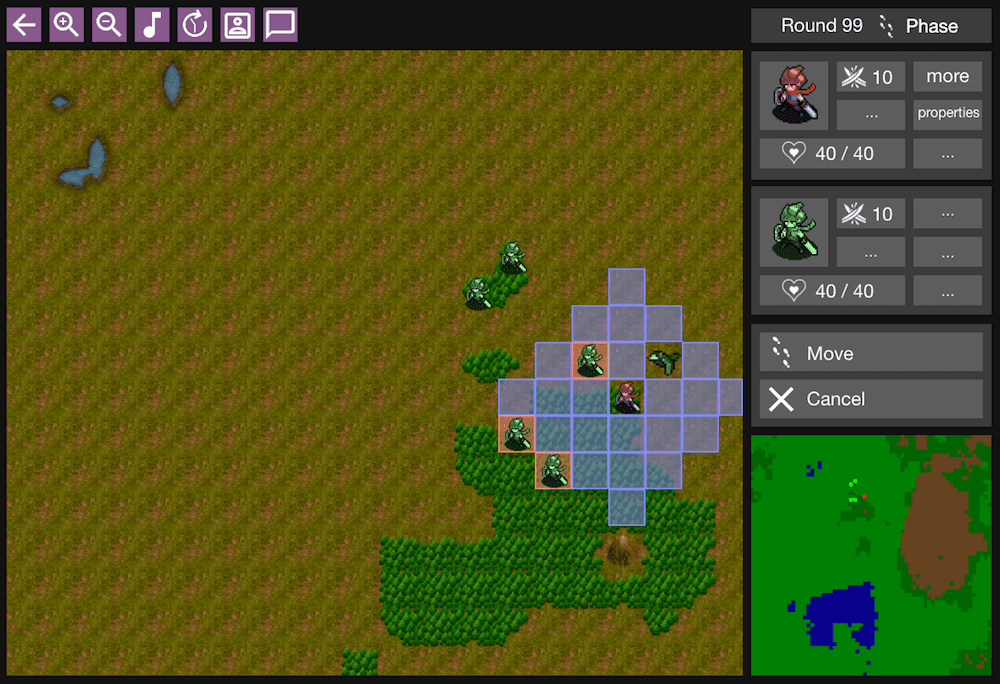
\includegraphics[width=0.8\textwidth]{images/mockups/Select.png}
    				    \caption{Mockup: Phase 1: Ausw"ahlen}
    				    \label{Select_1}
			        \end{figure}
			        \ \\ Nachdem alle drei Phasen vom aktiven Spieler beendet wurden, war die Runde des Spielers vorbei. Wenn der Nutzer selbst an der Reihe war und in einer seiner drei Phasen auf eine Einheit klickte, sollte der Bewegungsradius oder Angriffsradius angezeigt werden. Klickte der Nutzer wieder auf die bereits ausgew"ahlte Einheit, auf eine andere Einheit oder auf ein freies Feld sollte die Einheit nicht mehr ausgew"ahlt sein. \\
                    \begin{figure}[H] 
    				    \centering
    				    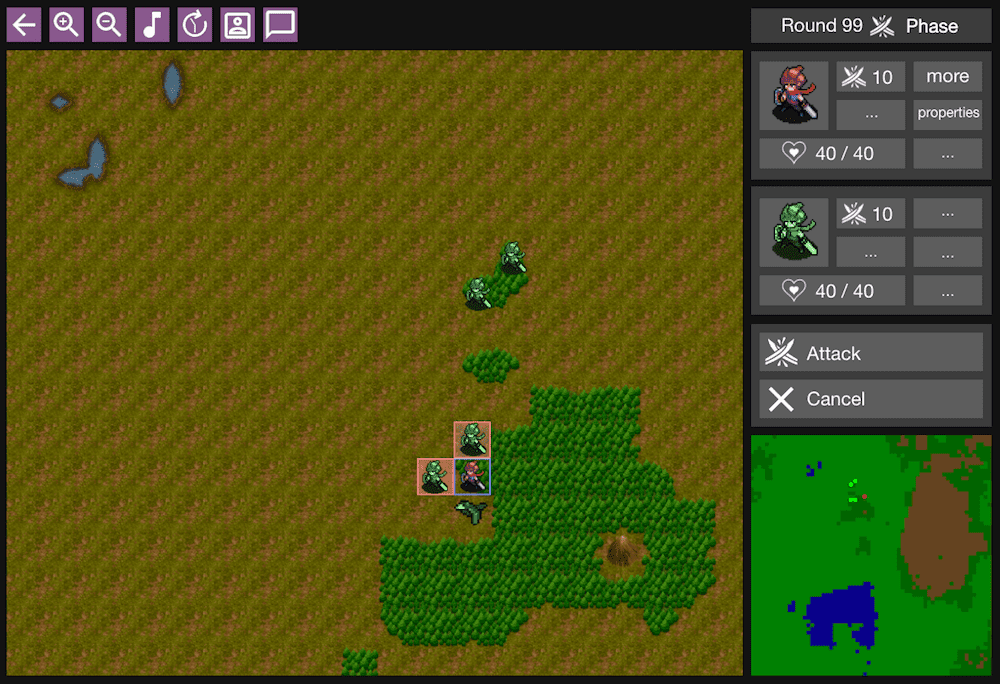
\includegraphics[width=0.8\textwidth]{images/mockups/Select3.png}
    				    \caption{Mockup: Phase 2: Ausw"ahlen}
    				    \label{Select_2}
			        \end{figure} 
			        \begin{figure}[H] 
    				    \centering
    				    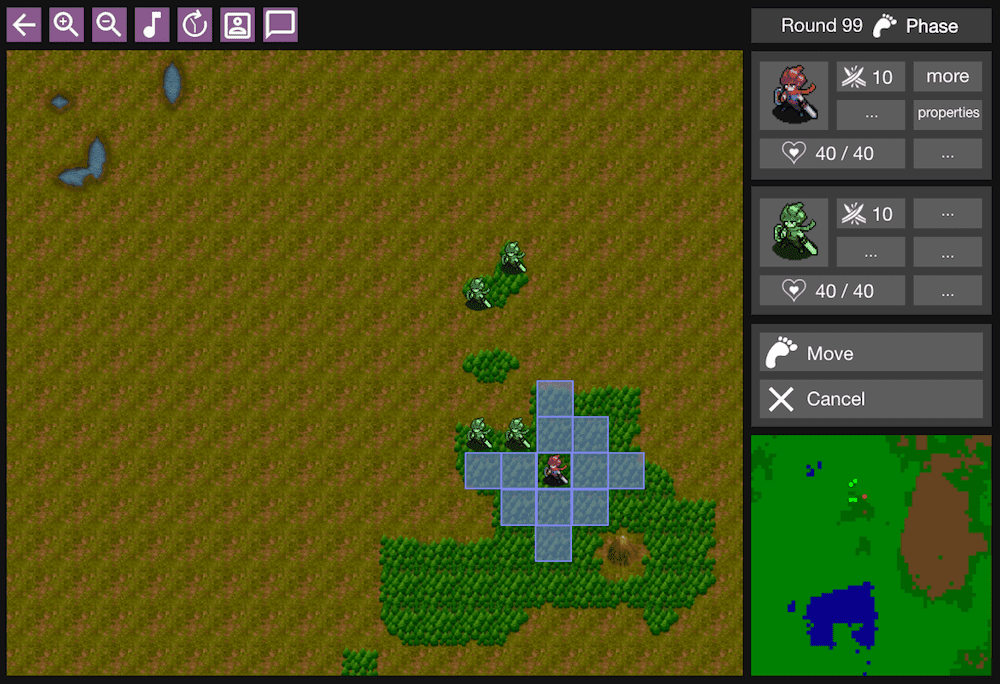
\includegraphics[width=0.8\textwidth]{images/mockups/Select2.png}
    				    \caption{Mockup: Phase 3: Ausw"ahlen}
    				    \label{Select_3}
			        \end{figure} 
		            \ \\ In einer gegnerischen Phase sollte die Einheit, die vom Gegner in seinem Client ausgew"ahlt wurde, auch beim Nutzer auf die selbe Art und Weise ausgew"ahlt werden. In Phase 1 sollten zus\"atzlich zum Bewegungsradius auch alle m"oglichen Angriffsziele markiert werden (siehe Abbildung \ref{Select_1}). In Phase 2 sollten nur alle m"oglichen Angriffsziele angezeigt werden (siehe Abbildung \ref{Select_2}). In Phase 3 sollte ein verk"urzter Bewegungsradius ohne Angriffsziele angezeigt werden (siehe Abbildung \ref{Select_3}), je nachdem wie weit sich eine Einheit noch bewegen konnte.
                \subsubsubsection{Einheit bewegen}
                    Nachdem der Nutzer in einer der Bewegungsphasen eine Einheit ausw"ahlte und auf ein Feld klickte, sollte die Einheit auf das Feld bewegt werden. Dazu sollte der k"urzeste Pfad berechnet und zum Server geschickt werden. Falls nach der Bewegung noch Bewegungspunkte "ubrig waren, sollte die Einheit weiterhin ausgew"ahlt bleiben und die Bewegungsreichweite dementsprechend verkleinert werden. War ein Gegner an der Reihe und der Server sandte die Bewegung einer Einheit, sollte auch zuerst die Bewegungsreichweite angezeigt werden und nach einer kurzen Verz\"ogerung die Einheit bewegt werden. Sp"ater sollte der Nutzer "uber eine Box in der Sidebar die M"oglichkeit haben, seinen Zug zu widerrufen. Dabei sollte auf dem angeklickten Feld ein Icon angezeigt werden, bis der Nutzer die Aktion best"atigte oder abbrach (siehe Abbildung \ref{Move} oder \ref{Move2}). War ein Gegner an der Reihe wurden der Text und das Icon in der Box nicht angezeigt.
                    \begin{figure}[H] 
                    	\centering
                    	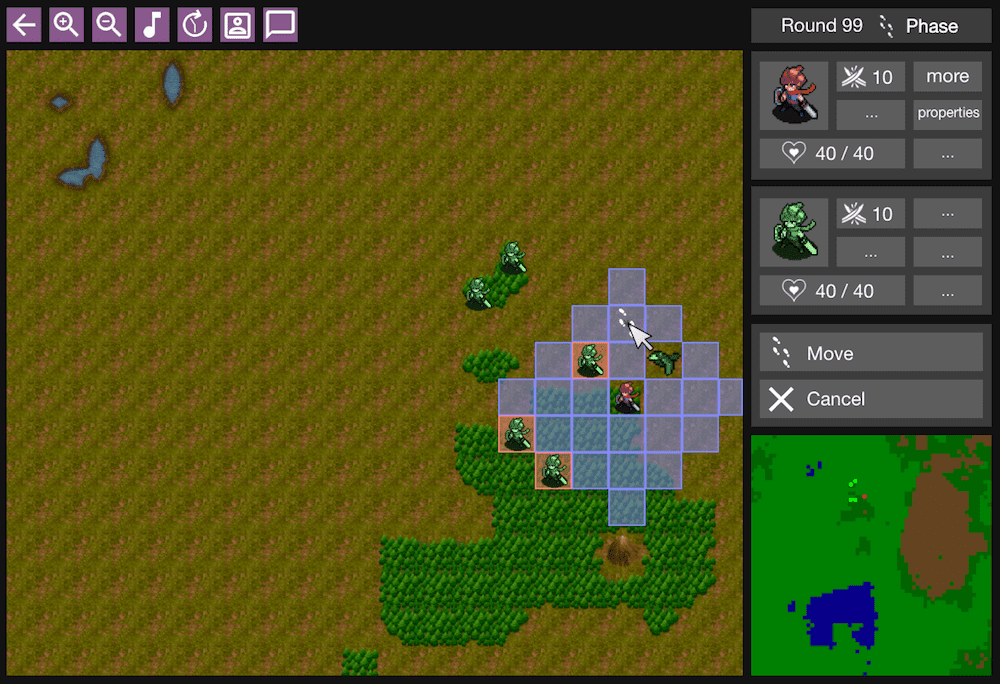
\includegraphics[width=0.8\textwidth]{images/mockups/ConfirmMove.png}
                    	\caption{Mockup: Bewegen best"atigen (Phase 1)}
                    	\label{Move}
                    \end{figure}
	                \begin{figure}[H] 
	                	\centering
	                	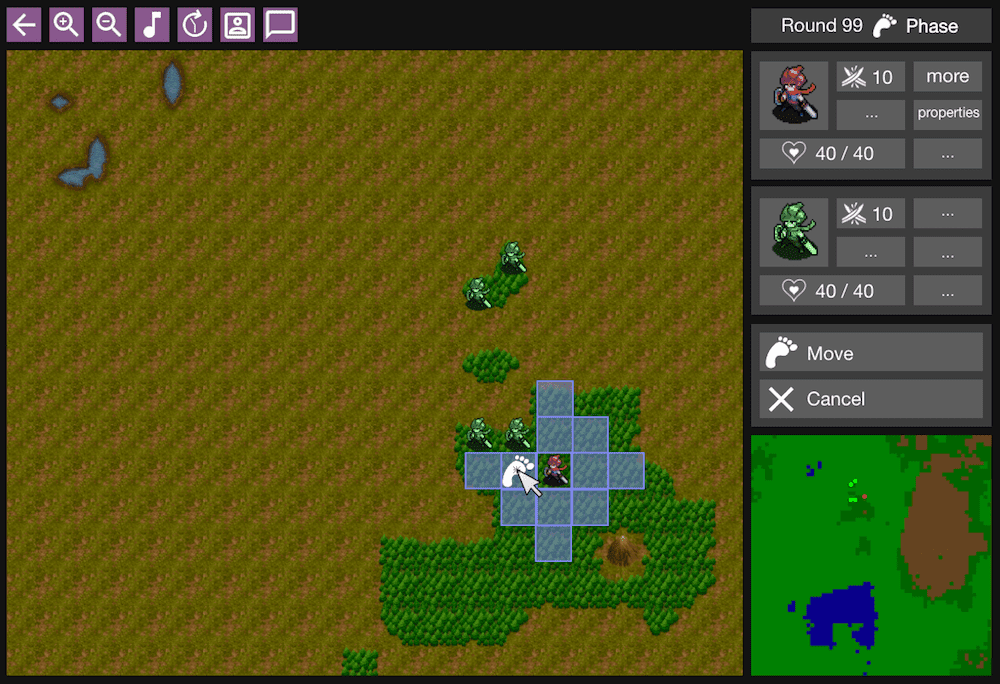
\includegraphics[width=0.8\textwidth]{images/mockups/ConfirmMove2.png}
	                	\caption{Mockup: Bewegen best"atigen (Phase 3)}
	                	\label{Move2}
	                \end{figure}
			    \subsubsubsection{Einheit angreifen}
			        Nachdem der Nutzer in der Angriffsphase eine Einheit ausw"ahlte und alle m"oglichen Angriffsziele angezeigt wurden, konnte er m\"ogliche Angriffsziele anklicken und angreifen. \\
			        \begin{figure}[H] 
    				    \centering
    				    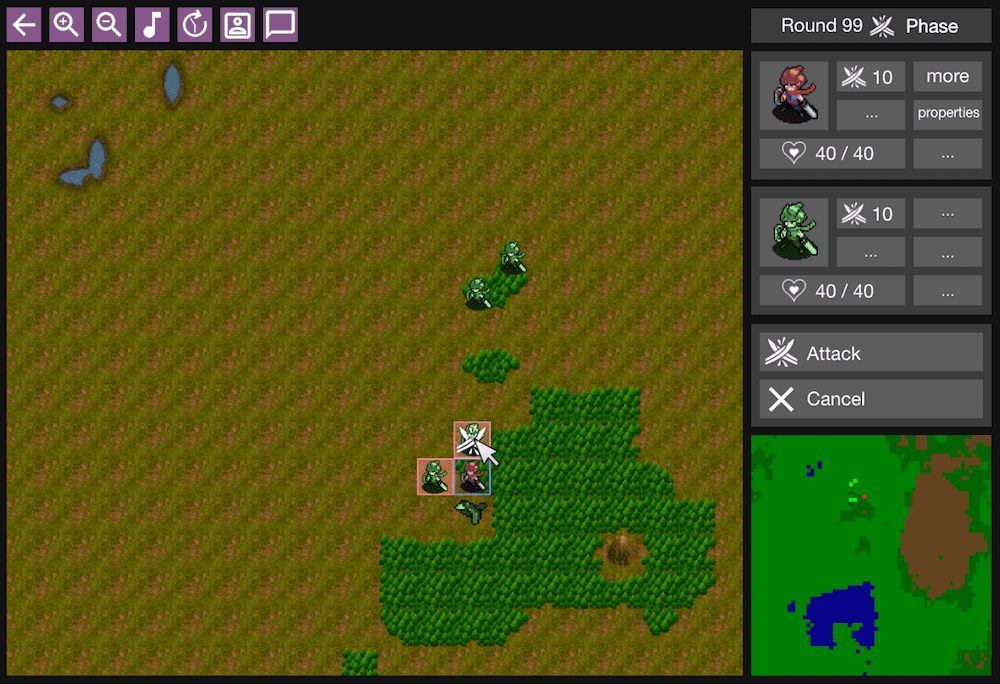
\includegraphics[width=0.8\textwidth]{images/mockups/Attack.png}
    				    \caption{Mockup: Angreifen best"atigen}
    				    \label{Attack}
			        \end{figure}
		        	\ \\ War ein Gegner an der Reihe und der Server sandte eine angegriffene Einheit, dann sollten auch zuerst die m"oglichen Angriffsziele angezeigt werden und nach einer kurzen Verz\"ogerung sollte die Einheit angreifen. Sp"ater sollte dies auch noch "uber eine Box in der Sidebar best"atigt werden, um dem Nutzer die M"oglichkeit zu geben, seinen Angriff doch nicht durchzuf"uhren. Dabei sollte auf dem angeklickten Feld ein Icon angezeigt werden, bis der Nutzer die Aktion best"atigte oder abbrach (siehe Abbildung \ref{Attack}). War ein Gegner an der Reihe, wurden der Text und das Icon in der Box nicht angezeigt.
			    \subsubsubsection{Spielende}
			        Wenn ein Spieler verlor, da er keine Einheiten mehr hatte, sollte sich Icon und Name seiner Spielerkarte schwarz f"arben. Der Client dieses Nutzers sollte ein Overlay angezeigen, welches ihm mitteilte, dass er verloren hatte. Au"serdem konnte er "uber das Overlay entscheiden, ob er zur"uck in die Lobby gehen oder in dem Spiel als Zuschauer bleiben wollte (siehe Abbildung \ref{Game_Lost}). Wenn nur noch ein Spieler "ubrig war, gewann dieser das Spiel. Diesem Nutzer sollte auch ein Overlay angezeigt werden, durch das er zur"uck zur Lobby wechselte (siehe Abbildung \ref{Game_Won}). Bei anderen Nutzern, die sich im Zuschauermodus befanden, sollte auch ein "ahnliches Overlay mit der gleichen Funktionalit"at angezeigt werden (siehe Abbildung \ref{Spectator_End}).
			        \begin{figure}[H] 
    				    \centering
    				    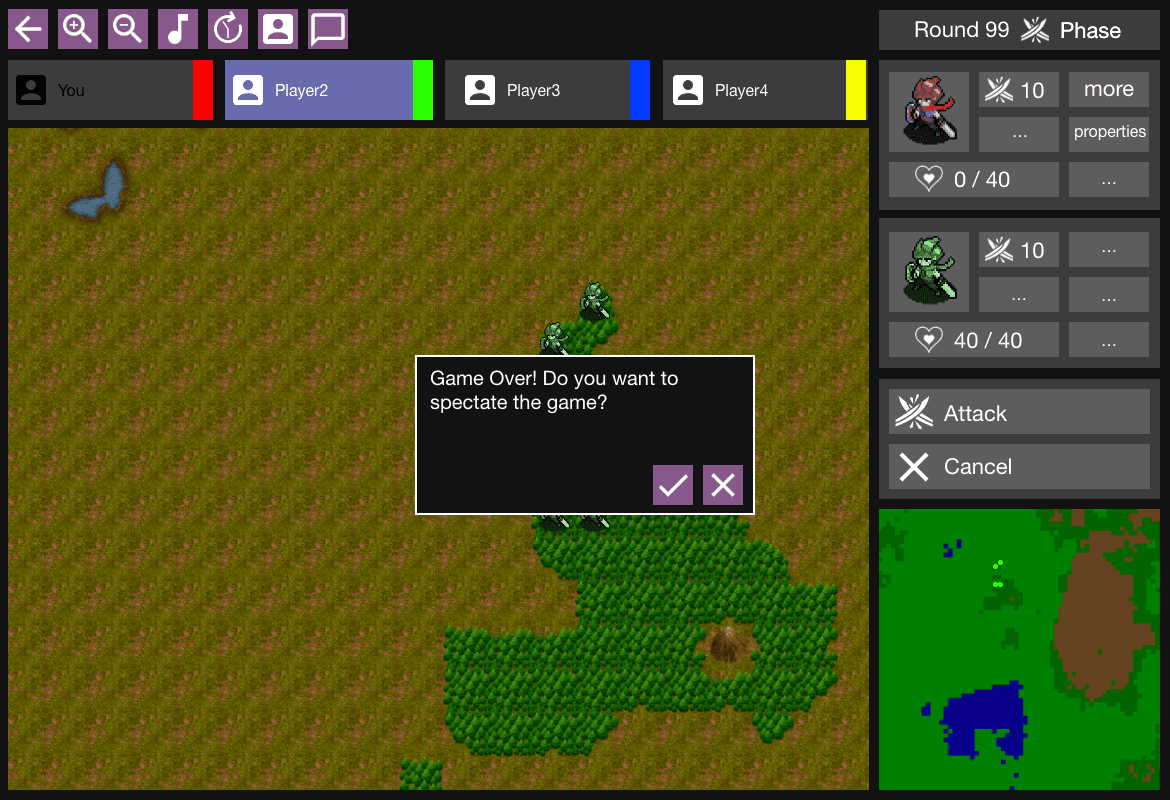
\includegraphics[width=0.8\textwidth]{images/mockups/GameOver.png}
    				    \caption{Mockup: Spiel verloren}
    				    \label{Game_Lost}
			        \end{figure}
			        \begin{figure}[H] 
    				    \centering
    				    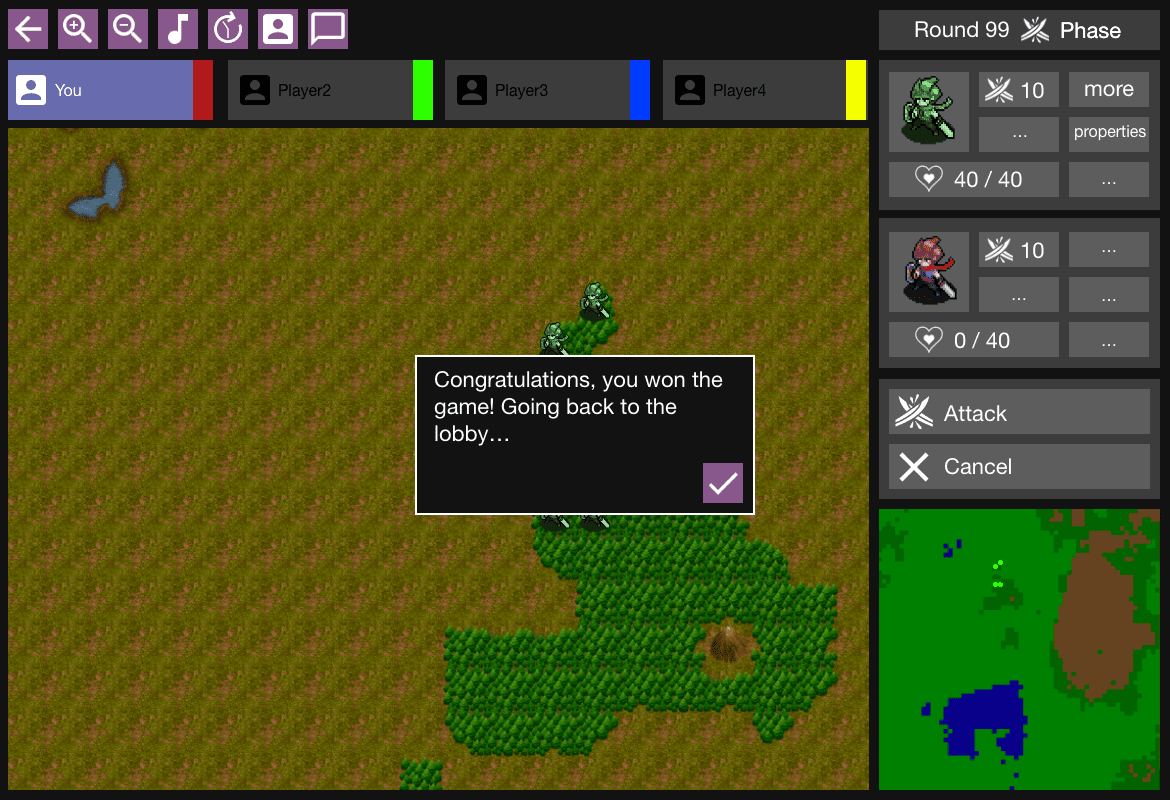
\includegraphics[width=0.8\textwidth]{images/mockups/GameWon.png}
    				    \caption{Mockup: Spiel gewonnen}
    				    \label{Game_Won}
			        \end{figure}
			        \begin{figure}[H] 
    				    \centering
    				    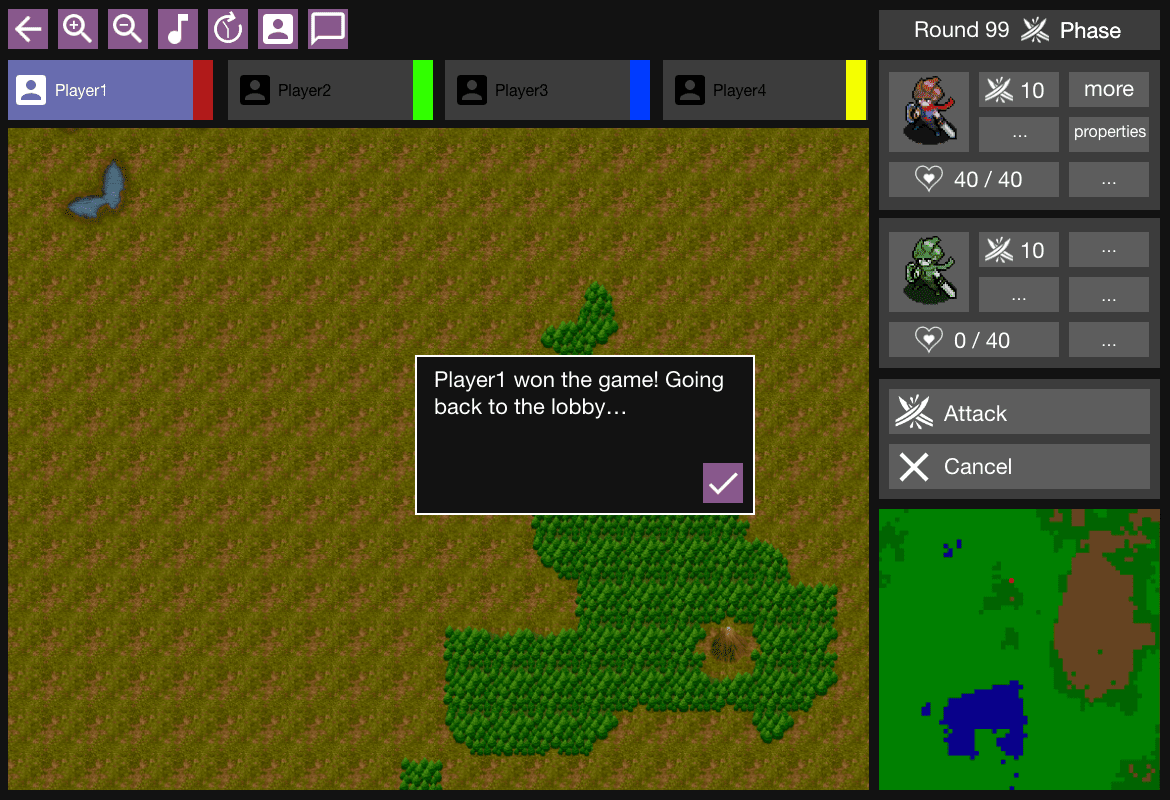
\includegraphics[width=0.8\textwidth]{images/mockups/SpectatorEnd.png}
    				    \caption{Mockup: Beobachtungsmodus: Spiel vorbei}
    				    \label{Spectator_End}
			        \end{figure}
			    \subsubsubsection{Weitere Features}
			        Es sollte f"ur den Nutzer m"oglich sein, "uber einen Button die Phase beenden zu k"onnen und in die n"achste zu wechseln. Nach Beenden aller drei Phasen, musste auch die Runde beendet werden. W\"ahrend ein Gegner an der Reihe war, war der Phase-Beenden-Button deaktiviert. Beim Beenden der Phasen sollte immer ein Overlay angezeigt werden (siehe Abbildung \ref{Phase_End}). \\
			        \begin{figure}[H] 
    				    \centering
    				    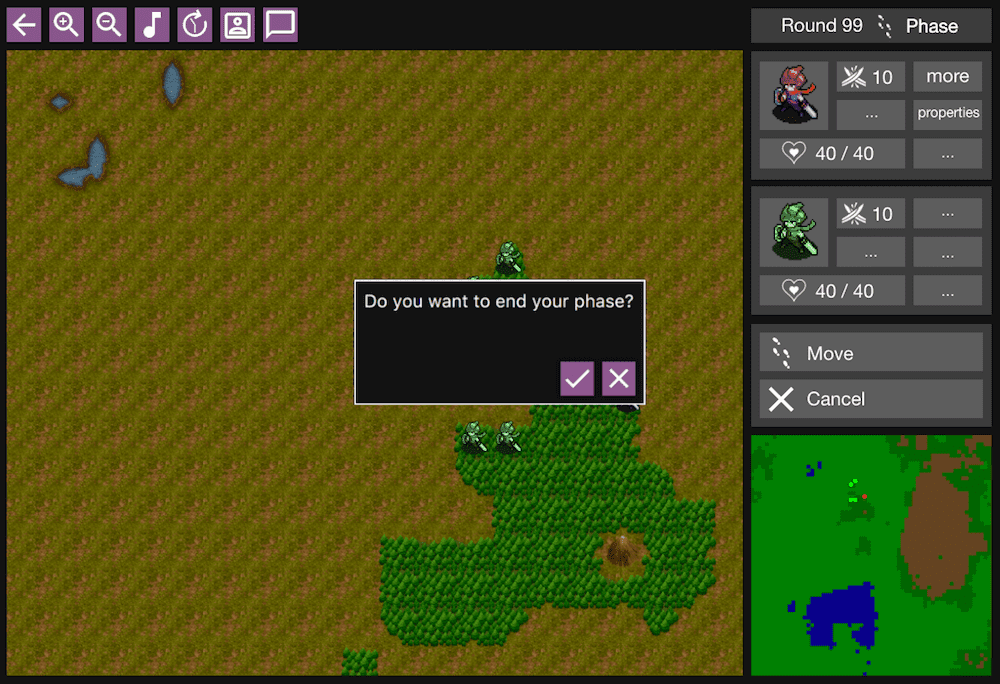
\includegraphics[width=0.8\textwidth]{images/mockups/EndPhase.png}
    				    \caption{Mockup: Phase beenden}
    				    \label{Phase_End}
			        \end{figure}
			        \ \\ Es gab ein weiteres Feature, bei dem der Nutzer "uber eine Einheit hovern konnte und deren Eigenschaften in der Sidebar angezeigt wurden. Die Einheiten des Spielers, der an der Reihe war, sollten in der oberen Box der Sidebar angezeigt werden. Die Einheiten der restlichen Spieler, die nicht an der Reihe waren, sollten in der unteren Box angezeigt werden. Zu Beginn jeder neuen Runde sollten die beiden Boxen leer sein und sich erst wieder f"ullen, wenn "uber eine Einheit gehovert beziehungsweise wenn eine Aktion mit einer Einheit ausgef"uhrt wurde.
		\subsection{Domain Stories}
		    Im Folgenden werden die Domain Stories f\"ur den Spielstart und das Ausf\"uhren einer Aktion, konkret die Bewegung einer Einheit, erl\"autert. Die Domain Stories wurden vor der Ver\"offentlichung der Serverdokumentation erstellt. Deshalb wichen die tats\"achlichen Nachrichten leicht von den hier aufgef\"uhrten Nachrichten ab. \\
		    \subsubsection{Spielstart}
		    	Der Nutzer tritt einem Spiel \"uber die Lobby bei. Der Client zeigt nun die initiale Spielsituation, die Armeeauswahl und alle Spieler, welche sich im Spiel befinden (siehe Abbildung \ref{Domain_Story_Ready_1}).
			    \begin{figure}[H] 
			    	\centering
			    	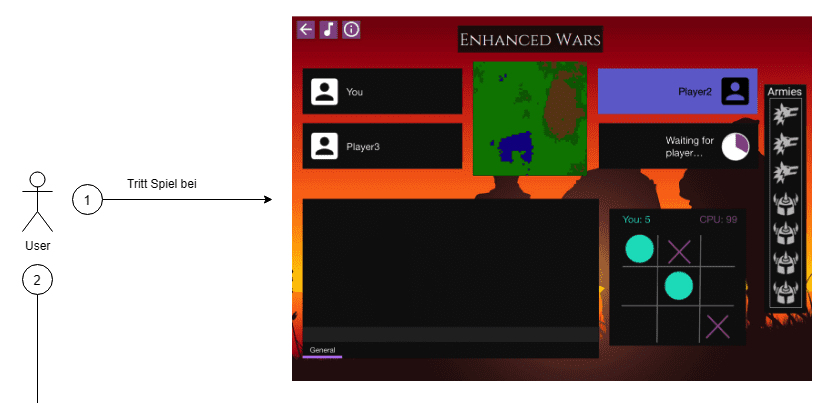
\includegraphics[width=\textwidth]{images/domain_stories/readyStory1.png}
			    	\caption{Domain Story: Ready 1}
			    	\label{Domain_Story_Ready_1}
			    \end{figure}
				\ \\ Der Nutzer w\"ahlt eine Armee aus. Die Spielerkarte des Nuzters wird aktualisiert und zeigt, dass er bereit ist (siehe Abbildung \ref{Domain_Story_Ready_2}).
			    \begin{figure}[H] 
			    	\centering
			    	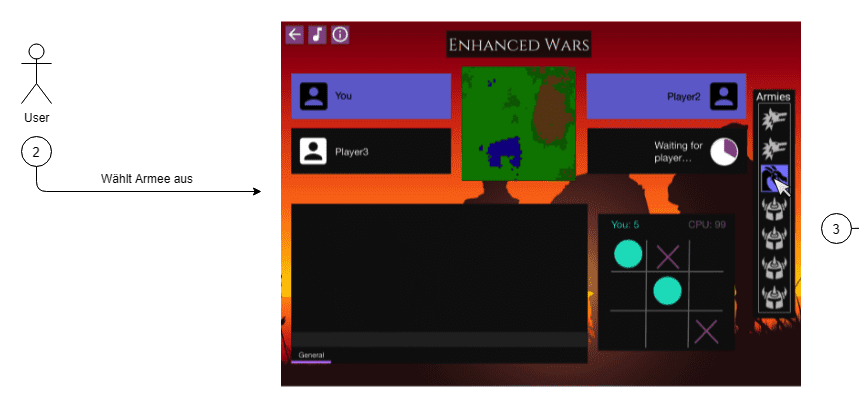
\includegraphics[width=\textwidth]{images/domain_stories/readyStory2.png}
			    	\caption{Domain Story: Ready 2}
			    	\label{Domain_Story_Ready_2}
			    \end{figure}
				\ \\ Die Anwendung teilt dem Server dann mit, dass der Nutzer bereit ist. Der Server informiert die Anwendung \"uber den Spielstart. Das Spiel startet (siehe Abbildung \ref{Domain_Story_Ready_3}).
		    	\begin{figure}[H] 
		    		\centering
		    		\includegraphics[width=\textwidth]{images/domain_stories/readyStory3.png}
		    		\caption{Domain Story: Ready 3}
		    		\label{Domain_Story_Ready_3}
		    	\end{figure}
		    \subsubsection{Bewegung}
		    	Der Nutzer klickt auf eine Einheit, wodurch diese  ausgew\"ahlt wird (siehe Abbildung \ref{Domain_Story_Move_1}).
		    	\begin{figure}[H] 
		    		\centering
		    		\includegraphics[width=\textwidth]{images/domain_stories/moveStory1.png}
		    		\caption{Domain Story: Move 1}
		    		\label{Domain_Story_Move_1}
		    	\end{figure}
				\ \\ Der Nutzer klickt auf ein g\"ultiges Zielfeld und best\"atigt die Aktion (siehe Abbildung \ref{Domain_Story_Move_2}).
		    	\begin{figure}[H] 
		    		\centering
		    		\includegraphics[width=\textwidth]{images/domain_stories/moveStory2.png}
		    		\caption{Domain Story: Move 2}
		    		\label{Domain_Story_Move_2}
		    	\end{figure}
				\ \\ Die Anwendung sendet eine Nachricht, welche die Bewegung beschreibt, an den Server. Dieser informiert die Anwendung \"uber die Zul\"assigkeit der Aktion. Die Anwendung aktualisiert das Datenmodell und das Benutzerinterface zeigt die neue Position der Einheit an (siehe Abbildung \ref{Domain_Story_Move_3}).
		    	\begin{figure}[H] 
		    		\centering
		    		\includegraphics[width=\textwidth]{images/domain_stories/moveStory3.png}
		    		\caption{Domain Story: Move 3}
		    		\label{Domain_Story_Move_3}
		    	\end{figure}
	\newpage
	\section{Sprint \RN{5}}
	    Der f"unfte Sprint erstreckte sich "uber dem Zeitraum vom 8.7.2019 bis zum 21.7.2019. Es wurden 116 Storypoints f"ur alle User Stories gesch"atzt.
	    \subsection{Sprintziel} \label{Sprintgoal_5}
	        Es sollte nach dem f"unften Sprint m"oglich sein:
	        \begin{itemize}
	            \item Einem Spiel beizutreten
	            \item Die Einheiten auf dem Spielfeld und der Minikarte zu sehen
	            \item Einheiten auszuw"ahlen, zu bewegen und anzugreifen
	            \item Den Spielstatus zu sehen und Phasen zu beenden
	        \end{itemize}
	        Falls die Entwicklung schneller als erwartet voranschreiten sollte, w"urden der Spielchat und das Spielende noch implementiert werden. Sollten alle Ziele abgeschlossen werden, w"urden "uber 80 Storypoints abgearbeitet werden, was bei vier Entwicklern als ein guter Fortschritt gewertet werden k"onnte.
	    \subsection{User Stories} \label{User_Stories_5}
	        Die User Stories, die vom Product Owner erstellt wurden, sind wie folgt aufgebaut: Dem Titel kann entnommen werden, zu welcher Szene die Story geh"orte. Anschlie"send werden die Story Points und der zugeteilte Entwickler genannt. Danach folgt die Story und das Ziel. Das Ziel fasst die Subtasks, die der Scrum Master erstellte, zusammen. Danach werden alle Subtasks aufgelistet. Falls die Story abgeschlossen wurde, wird der Verlauf und das Ergebnis dokumentiert. Falls die Story nur angefangen wurde, wird der Verlauf und der Stand dokumentiert.
	        \subsubsection{Warteraum - Spielbeitritt anpassen}
	            \paragraph{Zuteilung}
	                	Diese User Story wurde auf 5 Storypoints gesch\"atzt und an Omar Sood zugeteilt.
	            \paragraph{Story}
	            		Karli befindet sich in der Warteraumszene. Alle anderen Spieler sind bereit. Karli w"ahlt eine Armee aus. Da nun alle Spieler bereit sind, startet das Spiel (und es findet ein Szenenwechsel statt).
	            \paragraph{Ziel und Subtasks}
		         		Diese Tasks der User Story umfassen zum Gro"steil die Domain Story Spielstart. Der Spielbeitritt sollte an die Server\"anderungen angepasst werden. Das Ausw\"ahlen einer Armee sollte dem Server ein Bereit-Signal senden und das Spiel sollte starten, sobald alle Spieler bereit waren.
	                	\begin{enumerate}[label={}]
		                	\item \textbf{Armeeauswahl im Warteraum} \hspace{5pt} Die Armeeauswahl soll nur im Warteraum m"oglich sein. Daf"ur muss sie aus der Lobby entfernt und von der Armeeauswahl des Army Managers getrennt werden. Das Deaktivieren der Join/Create Game Buttons muss so angepasst werden, dass diese nur deaktiviert sind, wenn der Spieler keine einzige g"ultige Armee besitzt.
		                	\item \textbf{Ready-Funktionalit"at} \hspace{5pt} Spieler, die bereit sind, sollen im Warteraum hervorgehoben werden. W"ahlt ein Spieler eine Armee aus, signalisiert er gleichzeitig auch, dass er nun bereit ist.
		                	\item \textbf{Spielstart} \hspace{5pt} Sobald alle Spieler bereit sind (oder der Server eine entsprechende Nachricht sendet), soll das Spiel starten und ein entsprechender Szenenwechsel erfolgen. Der Websocket darf dabei nicht mehr terminiert werden, sondern soll f"ur den IngameController zur Verf"ugung stehen. (Bei einem Wechsel zur Lobby oder beim Schlie"sen der Anwendung muss der Socket nat"urlich weiterhin terminiert werden.)
	                \end{enumerate}
                \paragraph{Verlauf}
                	Diese Story nahm circa acht Stunden mehr in Anspruch. Das lag daran, dass das Trennen der neuen Box von der optisch identischen Armeeauswahlbox im Army Manager l"anger als gedacht dauerte. Dabei musste auch die neue Funktionalit"at (unter anderem Arme ausgew"ahlt = Ready) im Warteraum hergestellt werden.
                \paragraph{Ergebnis}
                	Der Spielstart funktionierte wie gew"unscht. Wenn der Server ein Ready eines Spielers sandte oder der Nutzer eine Armee ausw"ahlte, wurde seine Spielerkarte in der selected color markiert und das Spiel startete, sobald alle Spieler bereit waren. Es fehlte nur noch ein Lade-Indikator, bis der Sever das Spiel startete und ein Szenenwechsel stattfand. Weiterhin musste die Armeeauswahlbox noch auf die richtige Gr"o"se angepasst werden. Zu diesen beiden Aufgaben wurden Stories erstellt.
            \subsubsection{Ingame - Spielfeld}
	            \paragraph{Zuteilung}
	                	Diese User Story wurde auf 13 Storypoints gesch\"atzt und an Georg Siebert zugeteilt.
             	\paragraph{Story}
             		Karli befindet sich in der Spielszene. Karli sieht die Einheiten auf dem Spielfeld. Karli klickt auf ein Feld (einer Einheit). Das Feld wird ausgew"ahlt.
	            \paragraph{Ziel und Subtasks}
			   		Das Spielfeld sollte die Einheiten anzeigen. Jedes Feld musste anklickbar sein.
	            	 \begin{enumerate}[label={}]
	            		\item \textbf{Einheiten anzeigen} \hspace{5pt} Die Einheiten sollen angezeigt werden. "Andert sich die Position einer Einheit (im Datenmodell), soll sich auch das Spielfeld entsprechend aktualisieren.
	            		\item \textbf{OnClick-Extensionpoints} \hspace{5pt} Es soll m"oglich sein, beim Anklicken eines Feldes Methoden mit der Referenz der darunterliegenden Datenstruktur (der Cell Instanz) aufzurufen.
            		\end{enumerate}
            	\paragraph{Verlauf}
            		Diese Story wurde circa f"unf Stunden fr"uher abgeschlossen. Das lag daran, dass die Umbauarbeiten vom IngameController zum BattlefieldController und weitere kleinere Util Klassen zum Anzeigen der Assets schneller abgeschlossen wurden. Das Anklicken des Spielfeldes und das Setzen der Markierungen der Felder war auch leicht zu realisieren.
            	\paragraph{Ergebnis}
            		Feldern des Spielfeldes und der darauf eventuell stehenden Einheit lie"sen sich ausw"ahlen. Dazu wurden Property Bindings eingef"uhrt. Das jeweils ausgew"ahlte Feld wurde hellgrau mit einer Opazit"at hinterlegt. Hoverte der Nutzer "uber das ausgew"ahlte Feld mit einer Einheit, wurde sogar das n"achste Bild des idle Sprites angezeigt.
	        \subsubsection{Ingame - Phase beenden}
	            \paragraph{Zuteilung}
	                Diese User Story wurde auf 3 Storypoints gesch\"atzt und an Juri Lozowoj zugeteilt.
             	\paragraph{Story}
             		Karli befindet sich in der Spielszene. Karli klickt auf den Phase-Beenden Button. Die Phase wird beendet und die n"achste tritt ein (bzw. der n"achste Spieler ist an der Reihe).
	            \paragraph{Ziel und Subtasks}
	                Es sollte einen Button geben, welcher bei Bet\"atigung die aktuelle Phase beendete. Dies sollte nur m\"oglich sein, wenn der Nutzer an der Reihe war.
	            	\begin{enumerate}[label={}]
	            		\item \textbf{Button und Funktionalit"at hinzuf"ugen} \hspace{5pt} Bei der Bet"atigung des Buttons soll die aktuelle Phase beendet und der Server dar"uber informiert werden. Es soll nicht m"oglich sein, den Button zu bet\"atigen, wenn der Nutzer nicht an der Reihe ist.
	            	\end{enumerate}
            	\paragraph{Verlauf}
            		Den Button hinzuzuf"ugen und die Funktion herzustellen, nahm viel mehr Zeit in Anspruch, als daf"ur vorgesehen war. Es dauerte circa zw"olf Stunden l"anger. Der Grund daf"ur war, dass der Entwickler nach seiner Scrum Master Rolle im zweiten Release sich erst einmal wieder in die Projektstruktur einlesen musste. Weiterhin gab es immer wieder Probleme mit dem IngameViewTest. Das beheben dieser Probleme nahm viel Zeit in Anspruch.
            	\paragraph{Ergebnis}
            		Es gab nun einen Button, mit dem der Nutzer die Phase beenden konnte. Die dementsprechende Nachricht wurde an den Server geschickt. Au{\ss}erdem wurde der Button immer disabled, wenn der Nutzer nicht an der Reihe war oder wenn der Nutzer noch keine Bewegung in der ersten Phase machte.
            \subsubsection{Ingame - Einheit ausw\"ahlen} \label{story_select_unit}
	            \paragraph{Zuteilung}
	                	Diese User Story wurde auf 13 Storypoints gesch\"atzt und an Juri Lozowoj zugeteilt.
              	\paragraph{Story}
             		Karli befindet sich in der Spielszene. Karli w\"ahlt eine Einheit durch Klicken auf ihre Graphik aus. G"ultige Bewegungsziele werden blau und g"ultige Angriffsziele rot markiert.
	            \paragraph{Ziel und Subtasks}
	               	Durch Anklicken einer Einheit sollte diese ausgew\"ahlt werden. Danach musste die Bewegungs- und Angriffsreichweite sichtbar sein, je nachdem in welcher Phase der Nutzer sich befand.
	           		\begin{enumerate}[label={}]
	           			\item \textbf{Ausgew"ahlte Einheit setzen} \hspace{5pt} Klickt der Anwender auf eine Einheit, soll diese ausgew"ahlt werden (soll im Datenmodell bzw. Controller hinterlegt werden). Zudem soll die Zelle der Einheit farblich hervorgehoben werden. Dies soll nur m"oglich sein, wenn der Spieler an der Reihe ist.
	           			\item \textbf{G"ultige Ziele markieren} \hspace{5pt} G"ultige Bewegungs- und Angriffsziele (Cell, eventuell auch Unit) sollen als solche markiert werden (Property). Zudem sollen sie farblich hervorgehoben werden. Weiterhin darf in der Angriffsphase nur der rote Angriffsradius angezeigt werden und in der restlichen Bewegungspunkte Phase nur der blaue Bewegungsradius. Blau: \#868cfc f\"ur den Rahmen, beim Hintergrund 40\% Opacity (siehe selected color im Stylesheet). Rot: \#cf6679 f\"ur den Rahmen, beim Hintergrund 40\% Opacity (siehe error color im Stylesheet).
	           		\end{enumerate}
           		\paragraph{Verlauf}
           			Es wurden circa zw"olf Stunden an dieser Story gearbeitet, sodass noch circa eine Stunde zu der gesch"atzten Zeit "ubrig blieb. Die Funktion gab es bereits, jedoch wollte der Entwickler im n"achsten Sprint noch nach einem Fehler suchen, bei dem das UI nicht richtig markiert wurde.
           		\paragraph{Stand}
           			Beim Ausw"ahlen einer Einheit, wurde am Ende des f"unften Sprintes in den beiden Bewegungsphasen die Bewegungsreichweite blau angezeigt. In der Angriffsphase wurden alle Felder um die Einheit rot markiert. Es sollten weitere User Stories erstellt werden, um in der ersten Bewegungsphase auch die m"oglichen Angriffsziele anzuzeigen und um in der Angriffsphase nur die m"oglichen Angriffsziele anzuzeigen. Weiterhin sollte eine weitere Story erstellt werden, um in einer Bewegungsphase eine verk"urzte Bewegungsreichweite anzuzeigen, falls nach einer Bewegung noch Bewegungspunkte "ubrig waren.
            \subsubsection{Ingame - Einheit bewegen} \label{story_move_unit}
	            \paragraph{Zuteilung}
	                	Diese User Story wurde auf 13 Storypoints gesch\"atzt und an Omar Sood zugeteilt.
             	\paragraph{Story}
             		Karli befindet sich in der Spielszene. Karli w"ahlt eine Einheit aus, die Karli bewegen m"ochte. Karli klickt auf ein Feld in Bewegungsreichweite. Die Einheit wird bewegt.
	            \paragraph{Ziel und Subtasks}
				Die Tasks dieser Story setzten die Domain Story Bewegen um.
	                	F\"ur die Bewegung einer Einheit sollte der k\"urzeste Pfad zum Zielfeld berechnet werden. Anschlie"send musste eine Nachricht an den Server gesendet und dessen Antwort korrekt verarbeitet werden.
	            	\begin{enumerate}[label={}]
	            		\item \textbf{Berechnung des k"urzesten Weges} \hspace{5pt} Der Server erwartet einen g"ultigen Weg ohne Hindernisse. Daf"ur soll der Weg berechnet werden, der die geringste Anzahl an MP verbraucht.
	            		\item \textbf{Zug an Server senden} \hspace{5pt} Der Server soll "uber die Bewegung informiert werden.
	            		\item \textbf{Antwort des Servers verarbeiten} \hspace{5pt} Die Antwort des Servers soll korrekt verarbeitet werden. Das hei"st, dass im Erfolgsfall die Bewegung im Datenmodell umgesetzt werden soll und im Fehlerfall der User eine entsprechende Meldung erhalten soll.
	            		\item \textbf{Klickhandler} \hspace{5pt} Beim Klick auf ein als g"ultiges Bewegungsziel markiertes Feld soll die aktuell ausgew"ahlte Einheit dorthin bewegt werden.
	            		\item \textbf{Aufr"aumen} \hspace{5pt} Nach der Aktion soll aufger"aumt werden. Das hei"st, dass die zuvor ausgew"ahlte Einheit, welche die Aktion ausf"uhrt, nicht mehr ausgew\"ahlt sein soll. Es sollen keine Felder mehr hervorgehoben sein.
	            	\end{enumerate}
            	\paragraph{Verlauf}
            		Diese Story lag f"ur den f"unften Sprint gut in der Zeit. Von den 13 gesch"atzten Stunden, wurden vom Entwickler nur 35 Minuten als verbleibende Zeit eingetragen, obwohl sogar erst 11 Stunden und 19 Minuten gearbeitet wurde. Eigentlich gab es keine Probleme und die Story m"usste im n"achsten Sprint nur noch finalisiert werden.
            	\paragraph{Stand}
            		Die User Story war soweit mit all ihren Funktionalit"aten fertig. Die k"urzesten Pfade wurden berechnet und die Einheiten konnten auf das neue Feld bewegt werden. Der Entwickler wollte im n"achsten Sprint nur noch den Quellcode kontrollieren, Tests schreiben und beheben und Merge Konflikte l"osen.
            \subsubsection{Ingame - Einheit angreifen} \label{story_attack_unit}
	            \paragraph{Zuteilung}
	                Diese User Story wurde auf 5 Storypoints gesch\"atzt und an Omar Sood zugeteilt.
             	\paragraph{Story}
             		Karli befindet sich in der Spielszene. Karli w"ahlt eine Einheit aus. Karli sieht alle Felder mit Einheiten in Rot, die angegriffen werden k"onnen. Karli w"ahlt eine gegnerische Einheit auf diesen Feldern aus. Die Einheit wird angegriffen.
	            \paragraph{Ziel und Subtasks}
	                Es sollte m\"oglich sein, gegnerische Einheiten anzugreifen. Entsprechende Nachrichten sollten an den Server gesendet und dessen Antworten korrekt verarbeitet werden.
            		\begin{enumerate}[label={}]
            			\item \textbf{Angriff an Server senden} \hspace{5pt} Der Server soll "uber den Agriff informiert werden (Angreifende Einheit und angegriffene Einheit).
            			\item \textbf{Antwort des Servers verarbeiten} \hspace{5pt} Die Antwort des Servers soll korrekt verarbeitet werden. Das hei"st, dass im Erfolgsfall der Angriff im Datenmodell umgesetzt werden soll und im Fehlerfall der User eine entsprechende Meldung erhalten (zur Zeit sind keine Fehlerf"alle bekannt) soll.
            			\item \textbf{Klickhandler} \hspace{5pt} Beim Klick auf ein als g"ultiges Angriffsziel markiertes Feld soll, falls dort auch eine gegnerische Einheit positioniert ist, die aktuell ausgew"ahlte Einheit diese angreifen.
            			\item \textbf{Aufr"aumen} \hspace{5pt} Nach der Aktion soll aufger"aumt werden. Das hei"st, dass die zuvor ausgew"ahlte Einheit, welche die Aktion ausf"uhrt, nicht mehr ausgew"ahlt sein soll. Es sollen keine Felder mehr hervorgehoben sein.
            		\end{enumerate}
            \subsubsection{Ingame - Spielstatus anzeigen} \label{story_game_status}
	            \paragraph{Zuteilung}
	                Diese User Story wurde auf 8 Storypoints gesch\"atzt und an Tobias Klipp zugeteilt.
             	\paragraph{Story}
             		Karli befindet sich in der Spielszene. Karli sieht eine Runden- und Phasenanzeige. Karli klickt auf den Spieler-Anzeigen Button. Die Anzeige der Spieler wird eingeblendet. Der aktive Spieler ist hervorgehoben (in der selected-Color siehe Stylesheet bzw. Mockup).
	            \paragraph{Ziel und Subtasks}
	                Es sollte einen Button zum Ein- und Ausblenden der Spielerinformationen implementiert werden. Der aktive Spieler sollte hervorgehoben werden.
	            	\begin{enumerate}[label={}]
	            		\item \textbf{Rundenanzeige} \hspace{5pt} Die Rundenanzahl soll korrekt dargestellt und aktualisiert werden. Die aktuelle Phase soll angezeigt werden (Bewegungsphase, dann Angriffsphase, dann restliche Bewegungspunktephase). Die Phasen sollen neben dem Label mit einem Icon dargestellt werden. Laut Server befinden sich in einer Runde die drei verschiedenen Phasen.
	            		\item \textbf{Spielerliste} \hspace{5pt} Die Spielerliste soll alle Spieler, welche sich im Spiel befinden, und deren Farbe anzeigen. Der aktive Spieler soll hervorgehoben sein (in der selected Color). Spieler, welche das Spiel verlassen oder verloren haben, sollen mit einem schwarzen Icon und schwarzem Spielernamen hinterlegt sein.
	            		\item \textbf{Ein-/Ausblenden der Spielerliste} \hspace{5pt} "Uber einen Button in der oberen Leiste soll sich die Spielerliste ein- und ausblenden lassen.
	            	\end{enumerate}
            	\paragraph{Verlauf}
            		Zum Ende des f"unften Sprints wurden bereits circa zehn Stunden zu viel Zeit investiert. Das lag daran, dass es (l"anger als gedacht) dauerte, die Listener f"ur die Spielerkarten zu implementieren und die Spielerkarten richtig zu positionieren. Weiterhin nahm es Zeit in Anspruch, dass zwischen dem Runden- und Phasenlabel die Phase mit einem Icon dargestellt werden sollte. Dann ergaben sich zum Schluss des Sprints auch noch mehrere Merge Konflikte, da dieser Branch als letztes gemergt werden sollte, da die Arbeit hier l"anger dauerte. Somit gab es zwar alle Funktionalit"aten, jedoch konnte dieser Branch diesen Sprint noch nicht gemergt werden und wurde deshalb doch noch mit in den n"achsten Sprint genommen, um ihn zu finalisieren.
            	\paragraph{Ergebnis}
            		Das Ergebnis dieser Story war wie im Ziel beschrieben. Der Button zum Anzeigen der Spielerkarten und die Spielerkarten selbst waren vorhanden. Dazu wurde ein Listener implementiert, der die Spielerkarten aktualisierte. Das Label f"ur die Runden- und Phasenanzeige funktionierte auch und aktualisierte sich, wenn der Server die entsprechende Nachricht sandte oder der Nutzer "uber den Button von der User Story \glqq Ingame - Phase beenden\grqq\ die Phase bzw. die Runde beendete.
            \subsubsection{Ingame - Minikarte anzeigen} \label{story_minimap}
	            \paragraph{Zuteilung}
	                Diese User Story wurde auf 8 Storypoints gesch\"atzt und an Georg Siebert zugeteilt.
             	\paragraph{Story}
             		Karli befindet sich in der Spielszene. In der rechten oberen Ecke sieht Karli die Minikarte, welche neben dem Terrain auch alle Einheiten anzeigt. Karli dr"uckt den Minikarte Button. Die Minikarte wird ausgeblendet.
	            \paragraph{Ziel und Subtasks}
	                Es sollte eine Minikarte implementiert werden, die \"uber einen Button ein- und ausgeblendet werden konnte.
	            	\begin{enumerate}[label={}]
	            		\item \textbf{Minikarte anzeigen} \hspace{5pt} Die Minikarte soll, wie in der Story und den Mockups beschrieben, dargestellt werden.
	            		\item \textbf{Ein-/Ausblenden der Minikarte} \hspace{5pt} "Uber einen Button in der oberen Leiste soll sich die Minikarte ein- und ausblenden lassen.
	            	\end{enumerate}
            	\paragraph{Verlauf}
            		Obwohl die Story noch nicht abgeschlossen wurde, wurde die Zeitsch"atzung bereits "uberschritten. Es wurden schon 25 Minuten mehr gearbeitet. Die Funktionalit"at gab es allerdings bereits. Die Story wurde nur noch nicht beendet, da sich ihre zweite Subtask am Ende des Sprints, genauso wie die Mockups \"anderten (Weitere Informationen folgen dazu im Kapitel \ref{changed_user_story_minimap}).
            	\paragraph{Stand}
            		Die Minikarte konnte am Ende des f"unften Sprints mit einem Button oben rechts angezeigt werden. Weiterhin zeigte sie das Terrain und die Einheiten der Spieler. Die Story wurde eigentlich abgeschlossen, jedoch sollte die Minikarte im n"achsten Sprint eine feste Position unten in der Sidebar bekommen und Springen "uber das Spielfeld sollte durch Klicken auf die Minikarte m"oglich gemacht werden.
            \subsubsection{Ingame - Chatintegration} \label{story_chat}
	            \paragraph{Zuteilung}
	                Diese User Story wurde auf 13 Storypoints gesch\"atzt und an Tobias Klipp zugeteilt.
             	\paragraph{Story}
             		Karli befindet sich in der Spielszene. Karli dr"uckt den Chat-Einblenden Button. Der Chat wird angezeigt. Karli schreibt eine Nachricht. Die Nachricht wird im Chat f"ur alle Spieler im Spiel angezeigt. Bob schreibt eine Nachricht. Karli kann Bobs Nachricht lesen.
	            \paragraph{Ziel und Subtasks}
	                Es sollte einen Button zum Ein- und Ausblenden des Chats implementiert werden.
	            	\begin{enumerate}[label={}]
	            		\item \textbf{Nachrichten senden und empfangen} \hspace{5pt} Hinweis: Es sollte ausreichen, einen Chatnode 1:1 wie im WaitingRoomViewController zu instanziieren. Nachrichten sollen korrekt gesendet und empfangen werden (vgl. Warteraum und Lobbychat, siehe Serverdoku).
	            		\item \textbf{Ein-/Ausblenden des Chats} \hspace{5pt} "Uber einen Button in der oberen Leiste soll sich der Chat ein- und ausblenden lassen. Der Chat soll bis zur Sidebar rechts gehen. Der Chat ist in einer StackPane "uber dem Spielfeld (und die Sidebar ist ein anderes Element neben dem Spielfeld).
	            	\end{enumerate}
            \subsubsection{Ingame - Game Over} \label{story_game_over}
	            \paragraph{Zuteilung}
	                Diese User Story wurde auf 2 Storypoints gesch\"atzt und an Tobias Klipp zugeteilt.
             	\paragraph{Story}
             		Karli befindet sich in der Spielszene. Karlis Playerkarte f\"arbt sich schwarz (Name und Icon). Karli sieht ein Overlay aufgehen, auf welchem Karli gefragt wird, ob Karli das Spiel weiter betrachten m\"ochte. Karli dr\"uckt den Cancel Button. Karli wechselt in die Lobby.
	            \paragraph{Ziel und Subtasks}
	                Wenn der Nutzer verlor, sollte ein Overlay angezeigt werden. Auf diesem konnte er in die Lobby wechseln oder dem Spiel zuschauen.
	            	\begin{enumerate}[label={}]
	            		\item \textbf{Alert anlegen} \hspace{5pt} Der im Mockup zu sehende Alert soll angezeigt werden, falls der Nutzer das Spiel verliert (keine Einheiten) UND nicht gleichzeitig ein anderer Spieler dadurch gewinnt (In diesem Fall greift der Spectate Over Alert). Best"atigt der User die Anfrage, soll der Alert geschlossen werden. Tut er dies nicht, soll in die Lobby gewechselt werden. Achtung: Es kann immer nur ein Alert aktiv sein. Um daher sicherzustellen, dass dieser Alert angezeigt wird, m"ussen zuvor eventuell aktive Alerts geschlossen werden.
	            	\end{enumerate}
            \subsubsection{Ingame - Game Won} \label{story_game_won}
	            \paragraph{Zuteilung}
	                Diese User Story wurde auf 2 Storypoints gesch\"atzt und an Tobias Klipp zugeteilt.
             	\paragraph{Story}
             		Karli befindet sich in der Spielszene. Karli besiegt die letzte gegnerische Einheit. Karli sieht ein Overlay aufgehen. Karli wechselt in die Lobby.
	            \paragraph{Ziel und Subtasks}
                    Wenn der Nutzer gewann, sollte ein Overlay angezeigt werden, das ihn in die Lobby wechseln lie"s.
	            	\begin{enumerate}[label={}]
	            		\item \textbf{Alert anzeigen} \hspace{5pt} Der im Mockup zu sehende Alert soll angezeigt werden, falls der Nutzer das Spiel gewonnen hat. Bei Bet"atigung des Buttons soll in die Lobby gewechselt werden. Achtung: Es kann immer nur ein Alert aktiv sein. Um daher sicherzustellen, dass dieser Alert angezeigt wird, m"ussen zuvor eventuell aktive Alerts geschlossen werden.
	            	\end{enumerate}
             \subsubsection{Ingame - Spectator Over} \label{story_spectator_over}
             	\paragraph{Zuteilung}
             		Diese User Story wurde auf 2 Storypoints gesch\"atzt und an Tobias Klipp zugeteilt.
           		\paragraph{Story}
           			Karli befindet sich in der Spielszene. Bob besiegt die letzte gegnerische Einheit. Karli sieht ein Overlay aufgehen. Karli wechselt in die Lobby.
             	\paragraph{Ziel und Subtasks}
             		Wenn das Spiel vorbei war, sollte dem Nutzer ein Overlay angezeigt werden, durch das er in die Lobby wechselte.
             		\begin{enumerate}[label={}]
             			\item \textbf{Alert anzeigen} \hspace{5pt} Der im Mockup zu sehende Alert soll angezeigt werden, falls ein anderer Spieler (und nicht der Nutzer) das Spiel gewinnt. Bei Bet\"atigung des Buttons soll in die Lobby gewechselt werden. Achtung: Es kann immer nur ein Alert aktiv sein. Um daher sicherzustellen, dass dieser Alert angezeigt wird, m\"ussen zuvor eventuell aktive Alerts geschlossen werden.
             		\end{enumerate}
            \subsubsection{Lobby - Spectating} \label{story_lobby_spectating}
	            \paragraph{Zuteilung}
	                Diese User Story wurde auf 5 Storypoints gesch\"atzt und an Juri Lozowoj zugeteilt.
             	\paragraph{Story}
             		Karli befindet sich in der Lobbyszene.  Karli sieht die Spielliste und m"ochte dieses Mal nicht selbst spielen. Karli dr"uckt auf den Spectator-Button. Karli wird in die Warteraumszene weitergeleitet.
	            \paragraph{Ziel und Subtasks}
	                Es sollte ein Button hinzugef\"ugt werden, der einen Spielbeitritt als Beobachter erm\"oglichte.
	            	\begin{enumerate}[label={}]
	            		\item \textbf{Button hinzuf"ugen} \hspace{5pt} Jeder Eintrag in der Spielliste soll um den neuen Button erweitert werden. Bei Bet"atigung dieses Buttons soll ein Szenenwechsel in den Warteraum stattfinden, dieses Mal jedoch nur als Zuschauer.
	            	\end{enumerate}
            \subsubsection{Ingame - Spectating} \label{story_ingame_spectating}
	            \paragraph{Zuteilung}
	                Diese User Story wurde auf 13 Storypoints gesch\"atzt und an Juri Lozowoj zugeteilt.
             	 \paragraph{Story}
             		Karli befindet sich in der Spielszene. Karli versucht etwas in den Chat zu schreiben. Karli versucht Aktionen mit den Einheiten auszuf\"uhren. Karlis Aktionen funktionieren nicht. Karli merkt aber, dass alles andere funktioniert, holt Popcorn und genie"st das Spiel.
	            \paragraph{Ziel und Subtasks}
	                Das Spiel sollte so angepasst werden, dass ein Zuschauer weder mit dem Spielfeld interagieren, noch Chatnachrichten schreiben konnte.
	           		\begin{enumerate}[label={}]
	           			\item \textbf{Zuschauerfunktionalit"at hinzuf"ugen} \hspace{5pt} Die Szene soll der regul"aren Spielszene (ohne Runde-Beenden Button) entsprechen. Der Benutzer soll jedoch keine Aktionen ausf"uhren k"onnen oder Nachricht absenden k"onnen. Das Lesen von Chatnachrichten soll m"oglich sein.
	           		\end{enumerate}
            \subsubsection{Ingame - Einheiteninformationen} \label{story_unit_properties}
	            \paragraph{Zuteilung}
	                Diese User Story wurde auf 8 Storypoints gesch\"atzt und an Georg Siebert zugeteilt.
             	\paragraph{Story}
             		Karli befindet sich in der Spielszene. Karli f"ahrt mit seinem Maus "uber eine Einheit. Alle wichtigen Informationen \"uber die Einheit werden in einem Kontextmen\"u angezeigt.
	            \paragraph{Ziel und Subtasks}
	                Bewegte der Nutzer die Maus \"uber eine Einheit, sollten alle verf\"ugbaren Informationen dieser Einheit in einem Kontextmen"u angezeigt werden.
	            	\begin{enumerate}[label={}]
	            		\item \textbf{UI Element f\"ur Informationen erstellen} \hspace{5pt} Es soll ein UI Element zur Anzeige der Informationen erstellt werden. Die Informationen sollten beinhalten: Alle Attribute der Einheit (nur bei den HP eine max/zurzeit Anzeige) und das idle gif der Einheit.
	            		\item \textbf{Informationen beim Hovern anzeigen} \hspace{5pt} Das bereits erstellte UI Element soll beim Hovern "uber eine Einheit eingeblendet werden. Ansonsten soll es wieder ausgeblendet werden.
	            	\end{enumerate}
            \subsubsection{Ingame - Musiksteuerung} \label{story_music}
	            \paragraph{Zuteilung}
	                Diese User Story wurde auf 3 Storypoints gesch\"atzt und an Omar Sood zugeteilt.
             	\paragraph{Story}
             		Karli befindet sich in der Spielszene und die Musik spielt. Karli klickt auf den Musik Button. Die Musik wird ausgeschaltet.
	            \paragraph{Ziel und Subtasks}
	                Es sollte ein Musik Button hinzugef\"ugt werden, mit dem sich die Musik genauso bedienen lie"s wie in den restlichen Szenen.
	            	\begin{enumerate}[label={}]
	            		\item \textbf{Button und Funktionalit"at hinzuf"ugen} \hspace{5pt} Es soll ein Button zur De-/Aktivierung der Musik hinzugef"ugt werden. Die Funktionalit"at soll die gleiche wie bei Login, Lobby und Warteraum sein. Das hei"st, dass die Einstellung szenen"ubergreifend erhalten bleiben soll.
	            	\end{enumerate}
        \subsection{Tasks} \label{Tasks_5}
            Die folgenden Tasks wurden keiner User Story zugeordnet. Die Tasks sind wie gefolgt aufgebaut: Zuerst kommt die Zeitsch"atzung und der zugeteilte Entwickler. Danach wird das Ziel der Task aufgelistet. Falls die Task abgeschlossen wurde, wird der Verlauf und das Ergebnis dokumentiert. Falls die Task nur angefangen wurde, wird der Verlauf und der Stand dokumentiert.
            \subsubsection{Servernachrichten} \label{task_server_messages}
            	\paragraph{Zuteilung}
            		Diese Task wurde auf 8 Zeitstunden gesch\"atzt und an Omar Sood zugeteilt.
            	\paragraph{Ziel}
            		Der Entwickler sollte alle restlichen Servernachrichten abfangen, die in keiner User Story ber\"ucksichtig wurden. Dazu geh\"orten unter anderem \"Anderungen des Datenmodells, welche durch Aktionen der Gegenspieler anfielen.
            \subsubsection{Einheiteninformationen im Datenmodell} \label{task_unit_properties}
            	\paragraph{Zuteilung}
            		Diese Task wurde auf 5 Zeitstunden gesch\"atzt und an Tobias Klipp zugeteilt.
            	\paragraph{Ziel}
            		Der Entwickler sollte die Enums UnitType und UnitTypeInfo zu einer Enum zusammenf\"ugen und musste darauf achten, dass alle Funktionalit\"aten erhalten blieben.
    \newpage
        \subsection{Zeit"ubersicht}
        	Diese \"Ubersicht zeigt alle Stories, welche im Rahmen der Ziele bearbeitet werden sollten. Wie zu erkennen ist, wurden nicht alle Stories abgeschlossen. Es wurden jedoch schon umfangreichere Grundlagen f\"ur Features des sechsten Sprints gelegt.
        	\begin{longtable}[H]{p{6cm} c c c c }
        			\label{Time_1}
       				\textbf{User Story} & \textbf{Soll Zeit} & \textbf{Ist Zeit} & \textbf{Noch Zeit} & \textbf{Entwickler} \\
       				\toprule
       				\endhead
       				Warteraum - Spielbeitritt anpassen & 5 h & 13 h 9 min &  & Omar Sood\\
       				Ingame - Spielfeld & 13 h & 8 h 22 min &  & Georg Siebert\\
       				Ingame - Phase beenden & 3 h & 15 h 20 min &  & Juri Lozowoj \\
       				Ingame - Einheit ausw"ahlen & 13 h & 11 h 46 min & 1h 14 min & Juri Lozowoj \\
       				Ingame - Einheit bewegen & 13 h & 11 h 19 min & 35 min & Omar Sood \\
       				Ingame - Einheit angreifen & 5 h &  & 5 h & Omar Sood \\
       				Ingame - Spielstatus anzeigen & 8 h & 18 h 45 min &  & Tobias Klipp \\
       				Ingame - Minikarte anzeigen & 8 h & 8 h 25 min & 4 h & Georg Siebert \\
       				Ingame - Chatintegration & 13 h &  & 13 h & Tobias Klipp \\
       				Ingame - Game Over & 2 h &  & 2 h & Tobias Klipp \\
       				Ingame - Game Won & 2 h &  & 2 h & Tobias Klipp \\
        			\caption{Zeit"ubersicht f"unfter Sprint}
        	\end{longtable}
        \subsection{Analyse}
        	Der f\"unfte Sprint endete am 21.7.2019. Das Team schaffte 29 der 116 gesch\"atzten Storypoints.
        	\subsubsection{Burndown}
	        	\begin{figure}[H] 
	        		\centering
	        		\includegraphics[width=\textwidth]{images/sprintV/burndown.png}
	        		\caption{Sprint \RN{5}: Burndown Diagramm}
	        		\label{Burndown_5}
	        	\end{figure}
        		\ \\ Wie im Burndown-Diagramm zu sehen ist, wurden diesen Sprint nur vier Stories mit einem Umfang von 29 Storypoints abgeschlossen (siehe Kapitel \ref{done_stories_5}). Wie Tabelle \ref{Time_1} zeigt, betrug die Arbeitszeit trotzdem 84 Stunden. Die Hauptursache war die Untersch\"atzung der Aufgabenumf\"ange, wodurch mehrere begonnene Stories in diesem Sprint nicht mehr abgeschlossen werden konnten und andere deutlich mehr Zeit als erwartet in Anspruch nahmen. Zudem f\"uhrte die in diesem Release h\"ohere Anzahl an blockierenden und relatierten Tasks zu einer insgesamt langsamereren Entwicklung, da sich die Entwickler h\"aufig miteinander absprechen mussten.
        	\subsubsection{Abgeschlossene Stories} \label{done_stories_5}
        		Es wurden bisher vier Stories abgeschlossen. Dies war weniger als erwartet, aber aufgrund komplexer Aufgaben nicht zu vermeiden. Im Kapitel \ref{User_Stories_5} wurden bereits alle User Stories mit Verlauf und Ergebnis dokumentiert, die abgeschlossen wurden. Trotzdem folgt in der Abbildung \ref{Done_5} noch einmal eine Liste mit den abgeschlossenen User Stories:
        		\begin{figure}[H] 
        			\centering
        			\includegraphics[width=\textwidth]{images/sprintV/doneIssues.png}
        			\caption{Sprint \RN{5}: Abgeschlossene Stories}
        			\label{Done_5}
        		\end{figure}
        	\subsubsection{Angefangene Stories}
        		Wie bereits in der Analyse des Burndowns erw\"ahnt wurde, wurden drei bereits begonnene Stories zum Ende des Sprints noch nicht abgeschlossen. Im Kapitel \ref{User_Stories_5} wurden bereits alle User Stories mit Verlauf und Stand dokumentiert, die angefangen wurden. Trotzdem folgt noch einmal eine Liste mit den begonnenen User Stories:
        		\begin{itemize}
        			\item Ingame - Einheit ausw"ahlen
        			\item Ingame - Einheit bewegen
        			\item Ingame - Minikarte anzeigen
        		\end{itemize}
        	\subsubsection{Nicht abgeschlossene Stories/Tasks}
        		Des Weiteren wurden neben den drei bereits angefangenen Stories noch weitere elf Stories beziehungsweise Tasks aufgrund von Zeitgr\"unden nicht angefangen und abgeschlossen (siehe Abbildung \ref{To_Do_5}). Diese Aufgaben waren nicht optional und sollten von unserem Team im n\"achsten Sprint bew\"altigt werden.
        		\begin{figure}[H] 
        			\centering
        			\includegraphics[width=\textwidth]{images/sprintV/openIssues.png}
        			\caption{Sprint \RN{5}: Nicht abgeschlossene Stories/Tasks}
        			\label{To_Do_5}
        		\end{figure}
        	\subsubsection{Fazit}
        		Die Ziele des Sprints wurden verfehlt. Um die Mindestanforderungen zu erreichen, m"usste das Entwicklerteam seine Produktivit\"at im sechsten Sprint deutlich steigern. Da die C0 Abdeckung (siehe Abbildung \ref{Coverage_5}) zum Ende des f\"unften Sprints bereits 79\% betrug, gab es bei der Qualit\"atssicherung keine Defizite.
        		\begin{figure}[H] 
        			\centering
        			\includegraphics[width=\textwidth]{images/sprintV/coverage.png}
        			\caption{Sprint \RN{5}: C0 Testabdeckung (Siehe Line, \%)}
        			\label{Coverage_5}
        		\end{figure} 
    \newpage
    \section{Sprint \RN{6}}
    	Der sechste Sprint erstreckte sich \"uber dem Zeitraum vom 22.7.2019 bis zum 4.8.2019. Er umfasste 87 Storypoints.
    	\subsection{Sprintziel}
    		Es sollte nach dem sechsten Sprint m\"oglich sein:
    		\begin{itemize}
    			\item Alle Features aus dem Sprint \RN{5} (siehe Kapitel \ref{Sprintgoal_5}) zu verwenden
    			\item Einen Spielchat zu benutzen
    			\item Verschiedene Overlays beim Spielende zu sehen
    			\item Einem Spiel als Beobachter beizutreten
    			\item Einheiteninformationen in einer Sidebar einzusehen
    			\item Die Musik auch im Spiel ein- und auszuschalten
    		\end{itemize}
    		F\"ur den Fall, dass die Mindestanforderungen vor Ende des Sprints abgeschlossen werden sollten, sollte eine Sidebar zum Spielfeld hinzugef\"ugt werden. Diese sollte es erm\"oglichen Aktionen, wie Bewegen oder Angreifen, zu best\"atigen und abzubrechen. Falls das Team die Umsetzung der oben genannten Features schaffen w"urde, w"aren die Mindestanforderungen jedoch bereits erf\"ullt.
    	\subsection{Ge\"anderte User Stories vom Sprint \RN{5}}
    		Die folgenden Stories des f\"unften Sprints wurden aktualisiert, da sich ihre Zuteilung oder Mockups "anderten. F"ur den Aufbau und falls die Stories abgeschlossen oder angefangen wurden, gilt dasselbe wie im ersten User Story Kapitel \ref{User_Stories_5}.
    		\subsubsection{Ingame - Minikarte anzeigen} \label{changed_user_story_minimap}
    			 \paragraph{Zuteilung}
    				Diese User Story wurde auf 8 Storypoints gesch\"atzt und an Georg Siebert zugeteilt. Diese Story wurde bereits im Sprint \RN{5} angefangen.
   				\paragraph{Ge\"anderte Story}
   					Karli befindet sich in der Spielszene. In der rechten unteren Ecke sieht Karli die Minikarte, welche neben dem Terrain auch alle Einheiten anzeigt. Karli dr"uckt auf eine Stelle in der Minikarte. Der Sichtbereich "andert sich zu dieser Stelle.
    			\paragraph{Ge\"andertes Ziel und Subtasks}
    				Es sollte eine Minikarte implementiert werden. \"Uber die Minikarte sollte es m\"oglich sein, den Sichtbereich zu wechseln.
    				\begin{enumerate}[label={}]
    					\item \textbf{Minikarte anzeigen} \hspace{5pt} Die Minikarte soll, wie in der Story und den Mockups beschrieben, dargestellt werden.
    					\item \textbf{Springen "uber die Minikarte} \hspace{5pt} Durch das Klicken auf eine Stelle auf der Minikarte soll der Sichtbereich auf dem Spielfeld verschoben werden.
    				\end{enumerate}
    			\paragraph{Verlauf}
    				Eigentlich arbeitete der Entwickler im f"unften Sprint schon die gesch"atzte Zeit von acht Stunden, da sich aber die Mockups "anderten, steckte der Entwickler diesen Sprint noch einmal circa vier Stunden Zeit in diese Story.
    			\paragraph{Ergebnis}
    				Die Minikarte konnte im Sprint \RN{5} bereits angezeigt werden. Am Ende dieses Sprints hatte sie aber nun eine fixe Position in der rechten unteren Ecke in der Sidebar und war nicht mehr oben rechts "uber einen Button ausblendbar. Weiterhin konnte der Nutzer durch Klicken auf die Minkarte zu dieser Position auf dem Spielfeld springen. Der momentane Sichtbereich des Spielfeldes wurde auch in der Minikarte angezeigt.
   			\subsubsection{Ingame - Einheiteninformationen}
   				\paragraph{Zuteilung}
   					Diese User Story wurde auf 8 Storypoints gesch\"atzt und an Georg Siebert zugeteilt.
				\paragraph{Ge\"anderte Story}
					Karli befindet sich in der Spielszene. Karli f"ahrt mit Karlis Maus "uber eine Einheit. Alle wichtigen Informationen "uber die Einheit werden in der Sidebar angezeigt.
   				\paragraph{Ge\"andertes Ziel und Subtasks}
   					Bewegte der Nutzer die Maus \ "uber eine Einheit, sollten alle verf\"ugbaren Informationen dieser Einheit in einer Sidebar angezeigt werden.
   					\begin{enumerate}[label={}]
   						\item \textbf{UI Element f\"ur Informationen erstellen} \hspace{5pt} Es soll ein UI Element zur Anzeige der Informationen erstellt werden. Die Informationen sollen beinhalten: Alle Attribute der Einheit (nur bei den HP eine max/zurzeit Anzeige) und das Bild der Einheit.
   						\item \textbf{Informationen beim Hovern anzeigen} \hspace{5pt} Das bereits erstellte UI Element soll beim Hovern "uber einer Einheit eingeblendet werden und eingeblendet bleiben, bis "uber eine neue Einheit gehovert wird. Die Einheit, die der Spieler ausgew"ahlt, soll in der oberen Box angezeigt werden. Die Einheit, "uber die er zuletzt hovert, soll in der unteren Box angezeigt werden.
   					\end{enumerate}
   				\paragraph{Verlauf}
   					Der Entwickler ben\"otigte 5 Stunden l\"anger als erwartet.
   				\paragraph{Ergebnis}
   					Das Ziel wurde umgesetzt. Zus\"atslich wurden das Spiel um ein- und ausschaltbare Lebensbalken f\"ur Einheiten erweitert.
  				\subsubsection{Ingame - Game Over}
  					\paragraph{Neue Zuteilung}
  						Diese User Story wurde auf 2 Storypoints gesch"atzt und an Juri Lozowoj neu zugeteilt.
					\paragraph{Story, Ziel und Subtasks}
						Siehe Kapitel \ref{story_game_over}
					\paragraph{Verlauf}
						Der Entwickler ben\"otigte eine Stunde zur Implementierung des Overlays.
					\paragraph{Ergebnis}
						Das Ziel wurde umgesetzt.
				\subsubsection{Ingame - Game Won}
					\paragraph{Neue Zuteilung}
						Diese User Story wurde auf 2 Storypoints gesch"atzt und an Juri Lozowoj neu zugeteilt.
					\paragraph{Story, Ziel und Subtasks}
						Siehe Kapitel \ref{story_game_won}
					\paragraph{Verlauf}
						Die gesch\"atzte Entwicklungsdauer wurde um 6 Minuten \"uberschritten.
					\paragraph{Ergebnis}
						Das Ziel wurde umgesetzt.
				\subsubsection{Ingame - Spectator Over}
					\paragraph{Neue Zuteilung}
						Diese User Story wurde auf 2 Storypoints gesch"atzt und an Juri Lozowoj neu zugeteilt.
					\paragraph{Story, Ziel und Subtasks}
						Siehe Kapitel \ref{story_spectator_over}
					\paragraph{Verlauf}
						Die Entwicklung dauerte 1 Stunde und 17 Minuten l\"anger als erwartet.
					\paragraph{Ergebnis}
						Das Ziel wurde umgesetzt.
   		\subsection{\"Ubernommene User Stories aus Sprint \RN{5}}
   			Weiterhin gab es auch User Stories aus dem f\"unften Sprint, welche noch nicht abgeschlossen wurden. Diese wurden mit in den sechsten Sprint \"ubernommen. F"ur den Aufbau und falls die Stories abgeschlossen oder angefangen wurden, gilt dasselbe wie im ersten User Story Kapitel \ref{User_Stories_5}.
   			\subsubsection{Ingame - Einheit ausw\"ahlen}
   				\paragraph{Zuteilung}
   					Diese User Story wurde auf 13 Storypoints gesch"atzt und an Juri Lozowoj zugeteilt. Diese Story wurde bereits im Sprint \RN{5} angefangen.
   				\paragraph{Story, Ziel und Subtasks}
   					Siehe Kapitel \ref{story_select_unit}
   				\paragraph{Verlauf}
   					An dieser Story wurde im Sprint \RN{5} schon circa zw"olf Stunden gearbeitet. Diesen Sprint brauchte der Enwickler noch circa vier Stunden l"anger, um ein Problem zu beheben. Dies dauerte so lange, da Klickevents im UI gedebuggt werden mussten. Damit dauerte die Story circa 3,5 Stunde l"anger.
   				\paragraph{Ergebnis}
   					Die Story wurde eigentlich schon im Sprint \RN{5} abgeschlossen, aber in diesem Sprint behob der Enwickler noch das Problem , dass die UI falsch markiert wurde, wenn eine Einheit ausgew"ahlt wurde. Schlussendlich konnten Einheiten ohne Probleme bewegt werden.
   			\subsubsection{Ingame - Einheit bewegen}
   				\paragraph{Zuteilung}
   					Diese User Story wurde auf 13 Storypoints gesch"atzt und an Omar Sood zugeteilt. Diese Story wurde bereits im Sprint \RN{5} angefangen.
   				\paragraph{Story, Ziel und Subtasks}
   					Siehe Kapitel \ref{story_move_unit}
   				\paragraph{Verlauf}
   					Im letzten Sprint wurde bereits circa elf Stunden an dieser Story gearbeitet. In diesem Sprint wurden noch circa zwei Stunden mehr gearbeitet, sodass es nur circa eine halbe Stunde l"anger dauerte, die Story abzuschlie"sen.
   				\paragraph{Ergebnis}
   					Eigentlich wurde diese Story auch im f"unften Sprint abgeschlossen. Im sechsten Sprint wurden nur noch minimale Anpassungen vorgenommen und Tests geschrieben.
   			\subsubsection{Ingame - Einheit angreifen}
   				\paragraph{Zuteilung}
   					Diese User Story wurde auf 5 Storypoints gesch"atzt und an Omar Sood zugeteilt.
   				\paragraph{Story, Ziel und Subtasks}
   					Siehe Kapitel \ref{story_attack_unit}
   				\paragraph{Verlauf}
   					Der Entwickler wurde circa zwei Stunden fr"uher fertig, da die Serverkommunikation, der Klickhandler und die Tests fr"uhzeitig abgeschlossen wurden.
   				\paragraph{Ergebnis}
   					Am Ende dieser Story war es m"oglich, gegnerische Einheiten neben der eigenen Einheit anzuklicken und anzugreifen. Weiterhin konnten diese Angriffe korrekt an den Server geschickt werden und auch vom Sever empfangen werden, falls ein Gegner eine Einheit angriff.
			\subsubsection{Ingame - Spielstatus anzeigen}
				\paragraph{Zuteilung}
					Diese User Story wurde auf 8 Storypoints gesch"atzt und an Tobias Klipp zugeteilt. 
				\paragraph{Story, Ziel und Subtasks}
					Siehe Kapitel \ref{story_game_status}
				\paragraph{Verlauf}
					Diese Story wurde im letzten Sprint Kapitel eigentlich bereits als abgeschlossen beschrieben, musste aber doch weiterhin ge\"offnet bleiben, da es mehrere Merge Konflikte zu l"osen gab. Eigentlich sch"atzte das Team nur acht Stunden, jedoch wurden im f"unften Sprint circa 18 Stunden und in dem sechsten Sprint circa noch einmal 13 Stunden Zeit investiert. Es musste noch einmal so viel Zeit aufgewendet werden, da andere Stories vor dieser Story gemergt wurden und somit sich viele Merge Konflikte ergaben, als der develop in diesen Branch gepullt wurde. Weiterhin funktionierten mehrere Tests danach nicht mehr, die ebenfalls behoben werden mussten.
				\paragraph{Ergebnis}
					Der Spielstatus wurde bereits im letzten Sprint korrekt angezeigt. Diesen Sprint wurden nur Konflikte behoben, die es nicht m"oglich machten, den Branch zu mergen.
			\subsubsection{Ingame - Chatintegration}
				\paragraph{Zuteilung}
					Diese User Story wurde auf 13 Storypoints gesch"atzt und an Tobias Klipp zugeteilt.
				\paragraph{Story, Ziel und Subtasks}
					Siehe Kapitel \ref{story_chat}
				\paragraph{Verlauf}
					Die Chatintegration wurde circa acht Stunden schneller abgeschlossen. Das lag daran, dass viele bereits vorhandene Chat Komponenten verwendet werden konnten.
				\paragraph{Ergebnis}
					Der Spielchat war "uber einen Button ausblendbar. Alle Spieler, die im Spiel waren konnten nun in unserem Client mit einander chatten. Der Chat wurde, wie auf den Mockups, unten links positioniert.
			\subsubsection{Lobby - Spectating}
				\paragraph{Zuteilung}
					Diese User Story wurde auf 5 Storypoints gesch"atzt und an Juri Lozowoj zugeteilt.
				\paragraph{Story, Ziel und Subtasks}
					Siehe Kapitel \ref{story_lobby_spectating}
				\paragraph{Verlauf}
					Der Entwickler war bereits nach etwa der H"alfte der Zeit fertig, da die Serverkommunikation doch einfach zu realisieren war.
				\paragraph{Ergebnis}
					In der Lobby sah der Nutzer neben jedem Spiel einen weiteren Button zum Beobachten des Spiels. Dr"uckte der Nutzer diesen Button wurde er als Beobachter in den Warteraum weitergeleitet, wo er wartete, bis das Spiel startete, um dem Spiel und den Spielern zuzuschauen.
			\subsubsection{Ingame - Spectating}
				\paragraph{Zuteilung}
					Diese User Story wurde auf 13 Storypoints gesch"atzt und an Juri Lozowoj zugeteilt.
				\paragraph{Story, Ziel und Subtasks}
					Siehe Kapitel \ref{story_ingame_spectating}
				\paragraph{Verlauf}
					Diese Story wurde bereits nach circa zwei Stunden abgeschlossen und brauchte deshalb viel weniger Zeit. Das lag daran, da das disablen von Aktionen und Buttons in der Spielszene schnell erledigt war.
				\paragraph{Ergebnis}
					War der Nutzer als Beobachter in der Spielszene, dann konnte er keine Aktionen (wie Bewegen und Angreifen) auf dem Spielfeld mehr durchf"uhren und auch keine Phasen mehr beenden.
			\subsubsection{Ingame - Musiksteuerung}
				\paragraph{Zuteilung}
					Diese User Story wurde auf 3 Storypoints gesch"atzt und an Omar Sood zugeteilt.
				\paragraph{Story, Ziel und Subtasks}
					Siehe Kapitel \ref{story_music}
				\paragraph{Verlauf}
					Die Musik lie"s sich nach 21 Minuten in der Spielszene bereits wieder steuern und die Story wurde viel schneller abgeschlossen. Es musste nur ein Button in der Szene hinzugef"ugt werden, da die Musik an sich bereits funktionierte.
				\paragraph{Ergebnis}
					Die Musik hatte nun einen Button, um jene auch in der Spielszene ein- und ausschalten zu k"onnen.
   		\subsection{User Stories}
   			Im sechsten Sprint wurden weitere User Stories vom Product Owner erstellt. F"ur den Aufbau und falls die Stories abgeschlossen oder angefangen wurden, gilt dasselbe wie im ersten User Story Kapitel \ref{User_Stories_5}.
   			\subsubsection{Ingame - Einheit bewegen nach Bewegung}
   				\paragraph{Zuteilung}
   					Diese User Story wurde auf 5 Storypoints gesch\"atzt und an Omar Sood zugeteilt.
  				\paragraph{Story}
  					Karli befindet sich in der Spielszene. Karli klickt auf eine Einheit. Die Bewegungsreichweite wird angezeigt. Karli klickt auf ein Feld in Bewegungsreichweite. Die Einheit wird bewegt und bleibt weiterhin ausgew"ahlt, aber der blaue Bewegungsradius hat sich verkleinert. Karli bewegt die Einheit noch einmal auf ein weiteres Feld. Die Bewegungspunkte sind noch nicht aufgebraucht und die Einheit bleibt weiter ausgew"ahlt. Karli hat keine Lust mehr die Einheit zu bewegen und w"ahlt sie ab.
   				\paragraph{Ziel und Subtasks}
   					Nachdem der Nutzer eine Einheit bewegte, sollte diese erneut ausgew\"ahlt sein, falls sie noch verbleibende Bewegungspunkte besa{\ss}.
   					\begin{enumerate}[label={}]
   						\item \textbf{Einheit ausw"ahlen} \hspace{5pt} Nachdem der Nutzer eine Einheit bewegt, soll diese erneut ausgew"ahlt werden, falls sie noch verbleibende Bewegungspunkte besitzt.
   					\end{enumerate}
   				\paragraph{Verlauf}
   					In dieser Story brauchte der Entwickler circa zwei Stunden l"anger, als die Zeit gesch"atzt wurde. Das lag daran, dass der Entwickler zum Ende der Story noch kleinere Bugs finden und beheben musste, bei denen verschiedene Ausnahmef"alle beim Ausw"ahlen einer Einheit nach der Bewegung beachtet werden mussten.
   				\paragraph{Ergebnis}
   					Das Bewegen wurde so erweitert, dass nach einer bereits ausgef"uhrten Bewegung die Einheit immer noch ausgew"ahlt war, wenn noch Bewegungspunkte zur Verf"ugung standen. Dementsprechend verkleinerte sich auch die blaue Bewegungsreichweite in der UI.
   			\subsubsection{Ingame - Einheit ausw"ahlen - Angriffsphase}
   				\paragraph{Zuteilung}
   					Diese User Story wurde auf 3 Storypoints gesch\"atzt und an Omar Sood zugeteilt.
   				\paragraph{Story}
   					Karli befindet sich in der Spielszene. Karli w\"ahlt eine Einheit durch Klicken auf ihre Graphik aus. Nur die g\"ultigen Angriffsziele, das hei"st, Felder bzw. Einheiten, welche in Reichweite sind, einem Gegner geh\"oren und von der ausgew\"ahlten Einheit angegriffen werden k\"onnen, werden rot markiert.
   				\paragraph{Ziel und Subtasks}
   					Nachdem der Nutzer in der Angriffsphase eine Einheit anklickte, sollten nur alle g\"ultigen Angriffsziele rot markiert werden.
   					\begin{enumerate}[label={}]
   						\item \textbf{Zielmarkierung "andern} \hspace{5pt} Es sollen nicht mehr alle benachbarten Felder, sondern nur noch g"ultige Angriffsziele farblich markiert werden.
   					\end{enumerate}
   				\paragraph{Verlauf}
   					Der Entwickler ben\"otigte zur Umsetzung die gesch\"atzte Zeit von 3 Stunden.
   				\paragraph{Ergebnis}
		   			Das Ziel wurde umgesetzt. G\"ultigte Angriffsziele wurden rot und ung\"ultige grau markiert.
		   	\subsubsection{Ingame - Einheit ausw"ahlen - Bewegungsphase}
		   		\paragraph{Zuteilung}
		   			Diese User Story wurde auf 5 Storypoints gesch\"atzt und an Omar Sood zugeteilt.
		   		\paragraph{Story}
		   			Karli befindet sich in der Spielszene. Karli w\"ahlt eine Einheit durch Klicken auf ihre Graphik aus. Neben der Bewegungsreichweite werden zus\"atzlich noch die g\"ultigen Angriffsziele rot markiert.
		   		\paragraph{Ziel und Subtasks}
		   			Nachdem der Nutzer in der Bewegungsphase eine Einheit anklickte, sollten auch alle g\"ultigen Angriffsziele in der Bewegungsreichweite rot markiert werden.
		   			\begin{enumerate}[label={}]
		   				\item \textbf{M"ogliche Angriffsziele markieren} \hspace{5pt} Es soll nicht nur die Bewegungsreichweite angezeigt werden, sondern auch alle g"ultigen Angriffsziele.
		   			\end{enumerate}
		   		\paragraph{Verlauf}
		   			Der Entwickler implementierte die Funktionalit\"at in 55 Minuten und unterschritt damit die erwartete Zeit deutlich.
		   		\paragraph{Ergebnis}
		   			G\"ultige Angriffsziele wurden auch in der Bewegungsphase rot markiert.
   		\subsection{Ge\"anderte Tasks vom Sprint \RN{5}}
   			Die folgenden Tasks des f\"unften Sprints wurden aktualisiert, da sich ihre Zuteilung "anderte. F"ur den Aufbau und falls die Tasks abgeschlossen oder angefangen wurden, gilt dasselbe wie im ersten Task Kapitel \ref{Tasks_5}.
   			\subsubsection{Einheiteninformationen im Datenmodell}
   				\paragraph{Neue Zuteilung}
   					Diese Task wurde auf 5 Zeitstunden gesch\"atzt und an Omar Sood neu zugeteilt.
   				\paragraph{Ziel}
   					Siehe Kapitel \ref{task_unit_properties}
   				\paragraph{Verlauf}
   					Die Umsetzung dieses Tasks verlief deutlich schneller als erwartet. Der Entwickler ben\"otigte nur 1 Stunde und 28 Minuten, da die Aufgaben doch leichter zu bew"altigen waren und das Test anpassen schnell ging.
   				\paragraph{Ergebnis}
   					Die Einheiteninformationen liegen nur noch in einer Enumeration vor. Erneute \"Anderungen der Einheiten-IDs f\"uhrten nicht mehr zu fehlerhaften Darstellungen und bei \"Anderungen ihrer Namen wurden diese als Fallback verwendet.
    	\subsection{\"Ubernommene Tasks aus Sprint \RN{5}}
    		Weiterhin gab es auch Tasks aus dem f\"unften Sprint, welche noch nicht abgeschlossen wurden. Diese wurden mit in den sechsten Sprint \"ubernommen. F"ur den Aufbau und falls die Tasks abgeschlossen oder angefangen wurden, gilt dasselbe wie im ersten Task Kapitel \ref{Tasks_5}.
			\subsubsection{Servernachrichten}
				\paragraph{Zuteilung}
					Diese Task wurde auf 8 Zeitstunden gesch\"atzt und an Omar Sood zugeteilt.
				\paragraph{Ziel}
					Siehe Kapitel \ref{task_server_messages}
				\paragraph{Verlauf}
					Diese Task wurde in Kombination mit der User Story Bewegen bearbeitet. Die Entwicklung verlief schneller als erwartet.
				\paragraph{Ergebnis}
					Alle Servernachrichten zum Aktualisieren des Datenmodells wurden korrekt verarbeitet.
   		\subsection{Tasks}
   			Im sechsten Sprint wurden weitere Tasks vom Scrum Master erstellt. F"ur den Aufbau und falls die Tasks abgeschlossen oder angefangen wurden, gilt dasselbe wie im ersten Task Kapitel \ref{Tasks_5}.
   			\subsubsection{Warteraum - Armeeauswahlbox anpassen}
   				\paragraph{Zuteilung}
   					Diese Task wurde auf 2 Zeitstunden gesch"atzt und an Tobias Klipp zugeteilt.
				\paragraph{Ziel}
					Die Gr"o"se der Box, in der das Element zur Armeeauswahl lag, sollte an das Element der Armeeauswahlbox angepasst werden.
				\paragraph{Verlauf}
					Der Entwickler ben\"otigte lediglich 30 Minuten, wodurch die erwartete Entwicklungsdauer um 1 Stunde und 30 Minuten unterschritten wurde. Das kam daher, da die Werte, die angepasst werden sollten, schnell im Code gefunden wurden.
				\paragraph{Ergebnis}
					Die H\"ohe der Armeeauswahlbox wurde angepasst und entsprach den Vorgaben.
			\subsubsection{Ingame - Best\"atigungsbox in der Sidebar}
				\paragraph{Zuteilung}
					Diese Task wurde auf 3 Zeitstunden gesch"atzt und an Georg Siebert zugeteilt.
				\paragraph{Ziel}
					Es musste eine Box in der Sidebar erstellt werden, die es m"oglich machte, Aktionen zu best"atigen oder abzubrechen (Die Funktionalit"aten sollten erst sp"ater in den untergeordneten User Stories erstellt werden). War der User nicht an der Reihe oder im Beobachtungsmodus, musste diese Box disabled werden. Beziehungsweise sollte dann auf den beiden Buttons der Text und das Icon nicht mehr sichtbar sein.
				\paragraph{Verlauf}
					Die Umsetzung des Tasks dauerte 30 Minuten, womit die erwartete Zeit um 2 Stunden und 30 Minuten unterschritten wurde.
				\paragraph{Ergebnis}
					Das Ziel wurde umgesetzt. 
			\subsubsection{Spectating - REST Anfrage}
				\paragraph{Zuteilung}
					Diese Task wurde auf 1 Zeitstunde gesch"atzt und an Juri Lozowoj zugeteilt.
				\paragraph{Ziel}
					Die REST Anfrage zum Beitreten eines Spiels sollte um einen optionalen Parameter erweitert werden (siehe Serverdoku).
				\paragraph{Verlauf}
					Der Entwickler ben\"otigte zur Bearbeitung dieses Tasks eine Stunde.
				\paragraph{Ergebnis}
					Der Client sandte nun eine der Serverdokumentation entsprechende REST-Anfrage, auch wenn diese nicht ben\"otigt wurde.
			\subsubsection{Default-Buttons setzen}
				\paragraph{Zuteilung}
					Diese Task wurde auf 3 Zeitstunden gesch"atzt und an Tobias Klipp zugeteilt.
				\paragraph{Ziel}
					Es sollten an mehreren Stellen Default-Buttons gesetzt werden, um als Nutzer schneller durch einige Fenster in der Anwendung zu kommen. Beim Best"atigungs-Alert (Confirm-Button), beim Info-Alert (Confirm-Button) und beim Phase beenden Button (Spielszene) sollten sie gesetzt werden.
				\paragraph{Verlauf}
					Die Implementierung dauerte 15 Minuten l\"anger als erwartet.
				\paragraph{Ergebnis}
					Alle Alerts sowie der Phase beenden Button lie{\ss}en sich mit der Best\"atigungstaste bedienen. Zus\"atzlich wurde das Bedienen des Abbrechen Buttons beim Best"atigungs-Alert mit der Escape Taste erm\"oglicht.
			\subsubsection{Ingame - Nicht ausw"ahlbar - Angriffsphase}
				\paragraph{Zuteilung}
					Diese Task wurde auf 3 Zeitstunden gesch"atzt und an Omar Sood zugeteilt.
				\paragraph{Ziel}
					Einheiten konnten nicht mehrmals angreifen. Deshalb sollten Einheiten, welche bereits einen Angriff t\"atigten, w\"ahrend dieser Angriffsphase nicht mehr ausw\"ahlbar sein.
				\paragraph{Verlauf}
					Die Umsetzung dauerte lediglich 5 Minuten.
				\paragraph{Ergebnis}
					Nach Absprache mit dem Product Owner wurde das Ziel leicht ge\"andert. Einheiten waren weiterhin ausw\"ahlbar, jedoch wurden alle Angriffsziele ung\"ultig.
		\subsection{Bugs}
			Bugstasks zum Beheben von Problemen wurden vom Scrum Master erstellt, da im Verlauf der Entwicklung und beim Testen des Clients der ein oder andere Fehler aufkam. Diese werden hier wie gefolgt beschrieben: Zuerst wird genannt, wer den Bug beheben sollte. Danach wird das Problem beschrieben, das den Bug darstellte. Bearbeitungszeit wurden bei den Bugtasks nicht gesch\"atzt. Falls der Bug in diesem Sprint behoben werden konnte, wird ein Fix dokumentiert. Ansonsten wird der aktuelle Stand dokumentiert.
			\subsubsection{Terminierung sicherstellen}
				\paragraph{Zuteilung}
					Dieser Bug sollte von Omar Sood behoben werden.
				\paragraph{Problem}
					Die Terminierung des GameEventSockets musste angepasst werden. Sie sollte nicht doppelt aufgerufen werden. Weiterhin sollte sie immer stattfinden, wenn der Nutzer die Anwendung schloss oder in die Lobby wechselte.
				\paragraph{Fix}
					Der Bug wurde vollst\"andig behoben.
			\subsubsection{Ingame - Einheit mehrmals ausw\"ahlen}
				\paragraph{Zuteilung}
					Dieser Bug sollte von Juri Lozowoj behoben werden.
				\paragraph{Problem}
					Falls der Nutzer eine Einheit ausw\"ahlte, abw\"ahlte und dann wieder ausw\"ahlte, ohne vorher eine andere Einheit ausgew\"ahlt zu haben, wurde sie danach als Angriffs- bzw. Bewegungsziel farblich markiert. Dies sollte nicht stattfinden.
				\paragraph{Fix}
					Der Entwickler ben\"otigte eine Stunden um das Problem zu beheben. Die Hervorhebung wurde danach immer korrekt gesetzt.
			\subsubsection{Spectating - Automatischer Wechsel zum Spielfeld}
				\paragraph{Zuteilung}
					Dieser Bug sollte von Juri Lozowoj behoben werden.
				\paragraph{Problem}
					Falls der Nutzer einem Spiel als Beobachter beitrat und dieses bereits startete, wechselte der Client nicht zum Spielfeld. Falls also das Spiel bereits startete (sollte an den vorhandenen Einheiten, der aktuellen Phase oder dem aktuellen Spieler am Datenmodell zu erkennen sein), sollte ein automatischer Wechsel zum Spielfeld stattfinden.
				\paragraph{Stand}
					Das Problem lie{\ss} sich nicht beheben. Es stellte sich als serverseitiges Problem heraus und dieser wurde erst nach Ende des 3. Releases aktualisiert.
			\subsubsection{Lobby - Spielbeitritt blockieren}
				\paragraph{Zuteilung}
					Dieser Bug sollte von Georg Siebert behoben werden.
				\paragraph{Problem}
					Falls ein Spiel bereits voll war, sollte kein Spielbeitritt mehr m\"oglich sein. Daf\"ur sollte der entsprechende Button deaktiviert werden (und aktiviert werden, falls wieder ein Platz frei wurde).
				\paragraph{Fix}
					Die Behebung dieses Problems dauerte 30 Minuten. Es war nicht mehr m\"oglich einem vollen Spiel beizutreten.
			\subsubsection{RunLoop bei "Anderungen im Spiel}
				\paragraph{Zuteilung}
					Dieser Bug sollte von Tobias Klipp behoben werden.
				\paragraph{Problem}
					W"ahrend der Nutzer sich im Spiel (Warteraum- oder Spielszene) befand, konnte es passieren, dass der JavaFX Thread in einen runLoop lief.
				\paragraph{Fix}
					Der Fehler wurde durch \"Anderungen am Datenmodell au{\ss}erhalb des UI-Threads verursacht. Alle Aktualisierungen des Modells wurden deshalb in den UI-Thread verlegt, wodurch das Problem behoben wurde.
			\subsubsection{CSS Fehler}
				\paragraph{Zuteilung}
					Dieser Bug sollte von Tobias Klipp behoben werden.
				\paragraph{Problem}
					An verschiedenen Stellen (Create Game Fenster, Spielchat, Spielerkarten im Warteraum) kam es vor, dass manchmal der Stylesheet nicht richtig geladen oder verwendet wurde. Der eigentlich wei{\ss}e Text war beispielsweise schwarz oder der selected color Hintergrund (Spielerkarte, falls der Spieler bereit war) wurde durchsichtig.
				\paragraph{Stand}
					Es konnte keine L\"osung vor Ende des Releases gefunden werden.
   	\newpage
    	\subsection{Zeit\"ubersicht}
    		Die folgende Tabelle zeigt alle Stories, Tasks und Bugs (Trennstriche grenzen die drei Kategorien von einander ab), die in diesem Sprint bearbeitet werden sollten. Es wurden alle Issues bis auf die letzten beiden Bugs im Sprint \RN{6} fertiggestellt.
    		\begin{longtable}[H]{p{9cm} c c c }
    			\label{Time_2}
    			\textbf{Issue: User Story/Task/Bug} & \textbf{Soll Zeit} & \textbf{Ist Zeit} & \textbf{Entwickler} \\
    			\toprule
    			\endhead
    			Ingame - Einheit ausw\"ahlen & 13 h & 16 h 29 min & Juri Lozowoj \\
    			Ingame - Einheit bewegen & 13 h & 13 h 35 min & Omar Sood \\
    			Ingame - Einheit angreifen & 5 h & 3 h 15 min & Omar Sood \\
    			Ingame - Chatintegration & 13 h & 5 h & Tobias Klipp \\
    			Ingame - Minikarte anzeigen & 8 h & 12 h 14 min & Georg Siebert \\
    			Lobby - Spectating & 5 h & 2 h 21 min & Juri Lozowoj \\
    			Ingame - Spectating & 13 h & 2 h 13 min &  Juri Lozowoj \\
    			Ingame - Game Over & 2 h & 1 h  & Juri Lozowoj \\
    			Ingame - Game Won & 2 h & 2 h 6 min & Juri Lozowoj \\
    			Ingame - Spectator Over & 2 h & 3 h 17 min & Juri Lozowoj \\
    			Ingame - Einheiteninformationen & 8 h & 13 h & Georg Siebert \\
    			Ingame - Spielstatus anzeigen & 8 h & 31 h 30 min &  Tobias Klipp \\
    			Ingame - Musiksteuerung & 3 h & 21 min &  Omar Sood \\
    			Ingame - Einheit bewegen nach Bewegung & 5 h & 7 h 28 min & Omar Sood \\
    			Ingame - Einheit ausw"ahlen - Angriffsphase & 3 h & 3 h & Omar Sood \\
    			Ingame - Einheit ausw"ahlen - Bewegungsphase & 5 h & 55 min & Omar Sood \\
    			\midrule
    			Warteraum - Armeeauswahlbox anpassen & 2 h & 30 min & Tobias Klipp \\
    			Einheiteninformationen im Datenmodell & 5 h & 1 h 28 min & Omar Sood \\
    			Servernachrichten & 8 h & 1 min & Omar Sood \\
    			Ingame - Best\"atigungsbox in der Sidebar & 3 h & 30 min & Georg Siebert \\
    			Spectating - REST Anfrage & 1 h & 1 h & Juri Lozowoj \\
    			Default-Buttons setzen & 3 h & 3 h 15 min & Tobias Klipp \\
    			Ingame - Nicht ausw"ahlbar - Angriffsphase & 3 h & 5 min & Omar Sood \\
    			\midrule
    			Terminierung sicherstellen & - & 1 h 54 min & Omar Sood \\
    			Ingame - Einheit mehrmals ausw\"ahlen & - & 1 h & Juri Lozowoj \\
    			Lobby - Spielbeitritt blockieren & - & 30 min & Georg Siebert \\
    			RunLoop bei "Anderungen im Spiel & - & 0 & Tobias Klipp \\
    			Spectating - Autom. Wechsel zum Spielfeld & - & 2 h 30 min & Juri Lozowoj \\
    			CSS Fehler & - & 1 h 30 min & Tobias Klipp \\
    			\caption{Zeit\"ubersicht sechster Sprint}
    		\end{longtable}
    	\subsection{Analyse}
    		Der sechste Sprint endete am 4.8.2019. Das Team bew"altigte die initialen 87 sowie die nachtr\"aglich hinzugef\"ugten 13 Storypoints im Verlauf des Sprints.
	    	\subsubsection{Burndown}
	    		Wie dem Burndown-Diagramm zu entnehmen ist verlief die Entwicklung optimal. Die initialen Stories und Tasks wurden im erwarteten Zeitrahmen und ohne Verz\"ogerungen bearbeitet. Im Laufe des Sprints wurden deshalb weitere Stories und Tasks hinzugef\"ugt um das Produkt weiter zu verbessern. Auch diese wurden beendet.
	    		\begin{figure}[H] 
	    			\centering
	    			\includegraphics[width=\textwidth]{images/sprintVI/burndown.png}
	    			\caption{Sprint \RN{6}: Burndown Diagramm}
	    			\label{Burndown_6}
	    		\end{figure}
	    	\subsubsection{Abgeschlossene Stories}
	    		Alle verbleibenden User Stories aus dem Release \RN{3} wurden im Sprint \RN{6} abgeschlossen (siehe Abbildung \ref{Done_Stories_6}). Diese 15 Stories werden in der folgenden Abbildung \ref{Done_Stories_6} noch einmal aufgelistet:
	    		\begin{figure}[H]
	    			\centering
	    			\includegraphics[width=\textwidth]{images/sprintVI/doneStories.png}
	    			\caption{Sprint \RN{6}: Abgeschlossene Stories}
	    			\label{Done_Stories_6}
	    		\end{figure}
    		\subsubsection{Abgeschlossene Tasks}
    			Die Tasks aus dem Release \RN{3}, die keiner User Story zugeordnet waren, wurden auch alle im Sprint \RN{6} abgeschlossen (siehe Abbildung \ref{Done_Tasks_6}). Dazu geh"orten die "ubernommenen und die neuen Tasks aus dem Sprint \RN{6}. Diese sieben Tasks werden in der folgenden Abbildung \ref{Done_Tasks_6} noch einmal aufgelistet:
    			\begin{figure}[H]
    				\centering
    				\includegraphics[width=0.8\textwidth]{images/sprintVI/doneTasks.png}
    				\caption{Sprint \RN{6}: Abgeschlossene Tasks}
    				\label{Done_Tasks_6}
    			\end{figure}
    		\subsubsection{Behobene Bugs}
    			Im Laufe des Releases traten mehrere Bugs auf. Diese konnten fast alle behoben werden (siehe Abbildung \ref{Fixed_Bugs_6}). Die vier behobenen Bugs werden in der folgenden Abbildung \ref{Done_Tasks_6} noch einmal aufgelistet:
    			\begin{figure}[H]
    				\centering
    				\includegraphics[width=0.8\textwidth]{images/sprintVI/fixedBugs.png}
    				\caption{Sprint \RN{6}: Behobene Bugs}
    				\label{Fixed_Bugs_6}
    			\end{figure}
    		\subsubsection{Angefangene Bugtasks}
    			Es gab jedoch zwei Bugtasks, welche im Release \RN{3} nicht behoben werden konnten (siehe Abbildung \ref{Open_Bugs_6}). Dies waren \glqq Spectating - Automatischer Wechsel zum Spielfeld\grqq und \glqq CSS Fehler\grqq. Der Wechsel zum Spielfeld konnte nicht behoben werden, da ein Serverupdate n\"otig war welches nicht mehr im Release \RN{3} stattfand. Der CSS Fehler konnte mangels Entwicklungszeit nicht mehr behoben werden. Zudem trat am Ende des Release \RN{3} ein neuer Bug auf f\"ur den kein Issue mehr erstellt wurde. Dabei handelt es sich um einen Fehler welcher beim Verlassen eines Spiels unter bestimmten Umst\"anden auftrat, jedoch nicht zu einem Absturz der Anwendung f\"uhrte.
    			\begin{figure}[H]
    				\centering
    				\includegraphics[width=0.8\textwidth]{images/sprintVI/openBugs.png}
    				\caption{Sprint \RN{6}: Offene Bugs}
    				\label{Open_Bugs_6}
    			\end{figure}
	    	\subsubsection{Fazit}
	    		Der Sprint \RN{6} war erfolgreich und die gesetzten Ziele wurde erreicht. Das Team arbeitete dabei so effizient, dass weitere Funktionalit\"aten hinzugef\"ugt werden konnten. Die Behebung mehrerer Fehler f\"uhrte zudem zu einer deutlich stabileren Anwendung. Auch die Qualit\"atssicherung wurde eingehalten. Mit einer Testabdeckung von 82\% wurde die Mindestanforderung von 75\% \"ubertroffen.
	    		\begin{figure}[H] 
	    			\centering
	    			\includegraphics[width=\textwidth]{images/sprintVI/coverage.png}
	    			\caption{Sprint \RN{6}: C0 Testabdeckung (Siehe Line, \%)}
	    			\label{Coverage_6}
	    		\end{figure} 
	\newpage
	\section{Abschluss Release \RN{3}}
		Das dritte Release endete am 4.8.2018. Im letzten Kapitel werden die Mockups mit der aktuellen Implementation verglichen. Dabei wird insbesondere auf Unterschiede und fehlende Features eingegangen werden. Zuerst wird jedes Mal noch einmal das Mockup gezeigt, danach ein Bild vom Endstand des Releases. "Uber dem Mockup sollen jedes Mal die gesetzten Ziele stehen und "uber dem Endstand soll der Vergleich kommen.
		\subsection{Lobby}
			Es wurde gefordert, einem Beobachtungsmodus beitreten zu k"onnen. Au{\ss}erdem sollte die Armeeauswahlbox entfernt werden.
			\begin{figure}[H] 
				\centering
				\includegraphics[width=0.8\textwidth]{images/mockups/LobbyWatchMode.png}
				\caption{Mockup: Beobachtungsmodus Lobby}
				\label{Watch_Mode_2}
			\end{figure}
	\newpage
			\ \\ Wie auf der folgenden Abbildung \ref{End_Watch_Mode} zu sehen ist, wurden alle Anforderungen an der Lobby umgesetzt. Der Button zum Beitreten des Beobachtungsmodus wurde direkt neben den Button zum Beitreten des Spiels platziert.
			\begin{figure}[H] 
				\centering
				\includegraphics[width=0.8\textwidth]{images/endOfRelease/LobbyWatchMode.png}
				\caption{Endstand Release \RN{3}: Beobachtungsmodus Lobby}
				\label{End_Watch_Mode}
			\end{figure}
		\subsection{Warteraum}
			Es wurde gefordert, ein Ready Signal geben zu k"onnen. Darauf sollte die Spielerkarte in der secondary Farbe angezeigt werden. Das Icon und die Schrift sollte sich schwarz f"arben. Die Armeeauswahlbox sollte von der Lobby in den Warteraum umgezogen werden. Optionals waren das TicTacToe Spiel und der Spielname oben in der Mitte der Szene.
			\begin{figure}[H] 
				\centering
				\includegraphics[width=0.8\textwidth]{images/mockups/NotReady.png}
				\caption{Mockup: Nutzer nicht bereit}
				\label{Not_Ready_2}
			\end{figure}
			\ \\ Auf der folgenden Abbildung \ref{End_Not_Ready} ist zu erkennen, dass alle Features umgesetzt wurden bis auf die schwarze Schrift, wenn ein Spieler bereit war. Weiterhin fehlten die optionalen Features, da aus Zeitgr"unden zuerst einmal alle geforderten Features umgesetzt wurden. Wenn eine Armee ausgew"ahlt wurde, wurde das Icon in einem hellen Grauton hinterlegt, da diese Helligkeit besser zu verschiedenfarbigen Icons passte.
			\begin{figure}[H] 
				\centering
				\includegraphics[width=0.8\textwidth]{images/endOfRelease/NotReady.png}
				\caption{Endstand Release \RN{3}: Nutzer nicht bereit}
				\label{End_Not_Ready}
			\end{figure}
			\ \\  Au{\ss}erdem gab es ein optionales Feature, dass ein Indikator laden sollte, wenn das Spiel dabei war zu starten.
			\begin{figure}[H] 
				\centering
				\includegraphics[width=0.8\textwidth]{images/mockups/StartGame.png}
				\caption{Mockup: Spielstart}
				\label{Game_Start_2}
			\end{figure}
			\begin{figure}[H] 
				\centering
				\includegraphics[width=0.8\textwidth]{images/endOfRelease/StartGame.png}
				\caption{Endstand Release \RN{3}: Spielstart}
				\label{End_Game_Start}
			\end{figure}
			\ \\ Auf der Abbildung \ref{End_Game_Start} ist zu erkennen, dass beim Spielstart zum Ende des Releases noch kein Indikator lud, da dies optional war und somit noch nicht implementiert wurde.
		\subsection{Ingame}
			Es wurde gefordert, den Chat und die Spieler "uber einen Button einblenden zu k"onnen. Weiterhin sollten die Minikarte, Einheiteninformationen und ein Besta"atigen/Abbrechen Button in einer Sidebar enthalten sein. "Uber dieser Sidebar sollte die aktuelle Runde und Phase eingeblendet werden. Der aktuelle Spieler sollte in der secondary Farbe hinterlegt werden. Ein Musik Button sollte in der oberen Leiste hinzugef"ugt werden.
			\begin{figure}[H] 
				\centering
				\includegraphics[width=0.8\textwidth]{images/mockups/Ingame.png}
				\caption{Mockup: Ingame}
				\label{Ingame_View_2}
			\end{figure}
			\ \\ Wie auf den Abbildungen \ref{End_Ingame_View} und \ref{End_Ingame_View_2} zu sehen ist, wurden alle Features implementiert. Der einzige Unterschied lag darin, dass die UI au{\ss}erlich ein wenig abwich. Die Buttons in der oberen Leiste wurden in einer anderen Reihenfolge angeordent. Die Sidebar wurde ein wenig kleiner und dementsprechend auch alle Zellen der Einheiteninformationen. Die Minikarte war kleiner und der Besta"atigen/Abbrechen Button wurde in der primary Farbe hinterlegt (anstatt in Grau). Zus"atzlich wurde die Spielerfarbe bei den Einheiteninformationen angezeigt. Das Runden- und Phasenlabel lag ein wenig weiter unten. Die Spielerkarten waren ein wenig d"unner und da sie zusammen nicht die ganze Breite des Spielfeldes einnahmen, wurden sie mittig platziert.
			\begin{figure}[H] 
				\centering
				\includegraphics[width=0.8\textwidth]{images/endOfRelease/Ingame.png}
				\caption{Endstand Release \RN{3}: Ingame}
				\label{End_Ingame_View}
			\end{figure}
			\begin{figure}[H] 
				\centering
				\includegraphics[width=0.8\textwidth]{images/endOfRelease/Ingame2.png}
				\caption{Endstand Release \RN{3}: Ingame (Buttons nicht gedr"uckt)}
				\label{End_Ingame_View_2}
			\end{figure}
			\subsubsection{Einheit ausw"ahlen} \label{END_SELECT}
				Da es drei Phasen in einer Runde eines Spielers gab, wird dieses Kapitel der "Ubersicht halber kleiner geteilt. Ein Unterschied zur Zielsetzung war es in allen Phasen, dass die UI Markierungen eigentlich auch in den gegnerischen Phasen funktionieren sollte, wenn der Nutzer nicht an der Reihe war. Am Ende des Releases sah der Nutzer aber in den gegnerischen Phasen nur, wie sich Einheiten bewegten oder angegriffen wurden. Am Ende des dritten Releases wurde zus"atzlich noch das ausgew"ahlte Feld (bzw. die Einheit darauf) hellgrau hinterlegt. Das zuletzt gehoverte Feld wurde auch hellgrau hinterlegt. Die zuletzt gehoverte Einheit wurde in der unteren Einheitenbox in der Sidebar angezeigt und die ausgew"ahlte Einheit in der oberen Box (siehe bspw. Abbildung \ref{End_Ingame_View_2}).
				\subsubsubsection{Phase 1 - Bewegungsphase}
					In der ersten Phase sollten eigentlich nur die Bewegungsreichweite und alle m"oglichen Angriffsziele in dieser Reichweite angezeigt werden.
					\begin{figure}[H] 
						\centering
						\includegraphics[width=0.8\textwidth]{images/mockups/Select.png}
						\caption{Mockup: Phase 1: Ausw"ahlen}
						\label{Select_1_2}
					\end{figure}
					\ \\ Die Bewegungsreichweite wurde korrekt angezeigt. Jedoch werden alle m"oglichen Angriffsziele auf der gesamten Karte rot markiert (siehe Abbildung \ref{End_Select_1}). Ein weiteres zus"atzliches Feature war es, dass wenn der Nutzer nicht alle Bewegungspunkte aufbrauchte, die Einheit weiterhin ausgew"ahlt blieb und die Bewegungsreichweite sich in der UI verkleinerte. Waren die Punkte bei Null wurde die Einheit automatisch abgew"ahlt.
					\begin{figure}[H] 
						\centering
						\includegraphics[width=0.8\textwidth]{images/endOfRelease/Select.png}
						\caption{Endstand Release \RN{3}: Phase 1: Ausw"ahlen}
						\label{End_Select_1}
					\end{figure}
				\subsubsubsection{Phase 2 - Angriffsphase}
					In der zweiten Phase sollte nur die m"oglichen Angriffsziele rot markiert werden.
					\begin{figure}[H] 
						\centering
						\includegraphics[width=0.8\textwidth]{images/mockups/Select3.png}
						\caption{Mockup: Phase 2: Ausw"ahlen}
						\label{Select_2_2}
					\end{figure}
					\ \\ Es wurde zur Funktionalit"at der zweiten Phase nur erg"anzt, dass wenn eine Einheit neben der angreifenden Einheit nicht angegriffen werden konnte oder dort ein leeres Feld war, dieses Feld grau hinterlegt wurde (siehe Abbildung \ref{End_Select_2}). Wurde eine Einheit ausgew"ahlt, die bereits angriff, dann wurden alle Nachbarfelder grau angezeigt.
					\begin{figure}[H] 
						\centering
						\includegraphics[width=0.8\textwidth]{images/endOfRelease/Select3.png}
						\caption{Endstand Release \RN{3}: Phase 2: Ausw"ahlen}
						\label{End_Select_2}
					\end{figure}
				\subsubsubsection{Phase 3 - Bewegungsphase}
					In der dritten Phase sollte nur die Bewegungsreichweite angezeigt werden.
					\begin{figure}[H] 
						\centering
						\includegraphics[width=0.8\textwidth]{images/mockups/Select2.png}
						\caption{Mockup: Phase 3: Ausw"ahlen}
						\label{Select_3_2}
					\end{figure}
					\ \\ Die dritte Phase verhielt sich genauso wie die erste Phase (siehe Abbildung \ref{End_Select_3_2}). Also gab es hier auch kleine "Anderungen hingegen des Mockups.
					\begin{figure}[H] 
						\centering
						\includegraphics[width=0.8\textwidth]{images/endOfRelease/Select2.png}
						\caption{Endstand Release \RN{3}: Phase 3: Ausw"ahlen}
						\label{End_Select_3_2}
					\end{figure} 
			\subsubsection{Einheit bewegen und angreifen}
				Das Ausw"ahlen der Einheiten funktionierte wie vorgesehen, sogar in den Bewegungsphasen blieben die Einheiten ausgew"ahlt, wenn noch Bewegungspunkte "ubrig waren, wie schon im vorherigen Kapitel beschrieben. Die Mockups von Einheit bewegen und angreifen wurden allerdings nicht umgesetzt (siehe Kapitel 2.3.3.2 und 2.3.3.3). Geplant war es, den Besta"atigen/Abbrechen Button in der Sidebar zu benutzen, um Aktionen kontrollierter zu steuern. Wenn der Nutzer eine Einheit bewegen oder angreifen wollte, sollte zur Best"atigung ein Icon auf dem Feld erscheinen, auf das der Nutzer laufen wollte oder eine Einheit angreifen wollte. Die Buttons in der Sidebar waren also zum Ende des Releases ohne Funktion, aber die User Stories daf"ur wurden mit ins n"achste Release "ubernommen.
			\subsubsection{Spielende}
				Wenn ein Spieler aus dem Spiel ausschied, sollte sich sein Icon und sein Name auf der Spielerkarte schwarz f"arben. Dies wurde umgesetzt (siehe bspw. Abbildung \ref{End_Game_Won} oder \ref{End_Spectator_End}). Des Weiteren sollten bei den verschiedenen Spielenden verschiedene Overlays angezeigt werden.
				\subsubsubsection{Spiel gewonnen}
					Wenn alle Spieler bis auf der Nutzer aus dem Spiel ausgeschieden waren, sollte ein Overlay angezeigt werden, das den Nutzer informierte, dass er gewan. Danach sollte es ihn zur Lobby zur"uck schicken.
					\begin{figure}[H] 
						\centering
						\includegraphics[width=0.8\textwidth]{images/mockups/GameOver.png}
						\caption{Mockup: Spiel verloren}
						\label{Game_Lost_2}
					\end{figure}
					\ \\ Alles funktionierte, wie es geplant wurde. Die UI sah auch genauso wie auf den Mockups aus (vgl. Abbildung \ref{Game_Lost_2} und \ref{End_Game_Lost}).
					\begin{figure}[H] 
						\centering
						\includegraphics[width=0.8\textwidth]{images/endOfRelease/GameOver.png}
						\caption{Endstand Release \RN{3}: Spiel verloren}
						\label{End_Game_Lost}
					\end{figure}
				\subsubsubsection{Spiel verloren}
					Wenn der Nutzer aus dem Spiel ausgeschieden war, sollte ein Overlay angezeigt werden, das den Nutzer informierte, dass er verlor. Danach sollte es ihm die M"oglichkeit geben, entweder das Spiel weiter zu betrachten oder zur Lobby zur"uck zu gehen. Wenn der Nutzer der vorletzte Spieler im Spiel war, sollte das Overlay vom Beobachtungsmodus Ende angezeigt werden.
					\begin{figure}[H] 
						\centering
						\includegraphics[width=0.8\textwidth]{images/mockups/GameWon.png}
						\caption{Mockup: Spiel gewonnen}
						\label{Game_Won_2}
					\end{figure}
					\begin{figure}[H] 
						\centering
						\includegraphics[width=0.8\textwidth]{images/endOfRelease/GameWon.png}
						\caption{Endstand Release \RN{3}: Spiel gewonnen}
						\label{End_Game_Won}
					\end{figure}
					\ \\ Alles funktionierte, wie es geplant wurde. Die UI sah auch genauso wie auf den Mockups aus (vgl. Abbildung \ref{Game_Won_2} und \ref{End_Game_Won}).
				\subsubsubsection{Beobachtungsmodus Ende}
					Wenn alle Spieler bis auf einen Spieler aus dem Spiel ausgeschieden waren, sollte dem Nutzer ein Overlay angezeigt werden, das ihn informierte, dass ein Spieler gewan. Danach sollte es ihn zur Lobby zur"uck schicken.
					\begin{figure}[H] 
						\centering
						\includegraphics[width=0.8\textwidth]{images/mockups/SpectatorEnd.png}
						\caption{Mockup: Beobachtungsmodus: Spiel vorbei}
						\label{Spectator_End_2}
					\end{figure}
					\ \\ Alles funktionierte, wie es geplant wurde. Die UI sah auch genauso wie auf den Mockups aus (vgl. Abbildung \ref{Spectator_End_2} und \ref{End_Spectator_End}).
					\begin{figure}[H] 
						\centering
						\includegraphics[width=0.8\textwidth]{images/endOfRelease/SpectatorEnd.png}
						\caption{Endstand Release \RN{3}: Beobachtungsmodus: Spiel vorbei}
						\label{End_Spectator_End}
					\end{figure}
			\subsubsection{Weitere Features}
				Alle geplanten weiteren Features wie das Phase Ende und die Einheiteninformationen in der Sidebar, wenn eine Einheit ausgew"ahlt oder gehovert wurde (wie bereits zuvor in Kapitel \ref{END_SELECT} beschrieben), wurden umgesetzt.
				\begin{figure}[H] 
					\centering
					\includegraphics[width=0.8\textwidth]{images/mockups/EndPhase.png}
					\caption{Mockup: Phase beenden}
					\label{Phase_End_2}
				\end{figure}
				\subsubsubsection{Phase Ende}
					Der Nutzer sollte "uber einen Button in der oberen Leiste die Phase beenden k"onnen. Dazu sollte ein Overlay angezeigt werden und der Button sollte in gegnerischen Runden disabled sein. Alles funktionierte, wie es geplant wurde. Die UI sah auch genauso wie auf den Mockups aus (vgl. Abbildung \ref{Phase_End_2} und \ref{End_Phase_End}).
					\begin{figure}[H] 
						\centering
						\includegraphics[width=0.8\textwidth]{images/endOfRelease/EndPhase.png}
						\caption{Endstand Release \RN{3}: Phase beenden}
						\label{End_Phase_End}
					\end{figure}
				\subsubsubsection{Weitere hinzugekommene Features}
					Es gab auch noch ein paar neue Features, die im Verlauf des Releases \RN{3} hinzukamen, die in diesem Kapitel mit Mockups erw"ahnt werden sollen.
					\vspace{0.3cm} \newline
					Egal in welcher Phase der Nutzer war oder ob ein Gegner an der Reihe war, es war immer m"oglich auf eine gegnerische Einheit zu klicken und alle m"oglichen Angriffsziele dieser ausgew"ahlten Einheit rot hinterlegt zu sehen. Nicht angreifbare Einheiten wurden grau hinterlegt (siehe Abbildung \ref{End_Select_Enemy}).
					\begin{figure}[H] 
						\centering
						\includegraphics[width=0.8\textwidth]{images/endOfRelease/SelectEnemy.png}
						\caption{Endstand Release \RN{3}: Gegner ausw"ahlen}
						\label{End_Select_Enemy}
					\end{figure}
					\ \\ Ein weiteres nicht geplantes Feature war der Lebensbalken "uber jeder Einheit, der dem Nutzer leichter Bescheid gab, zu welchem Spieler die Einheit geh"orte. Weiterhin nahm die Farbe in dem Balken ab, wenn die Einheit weniger Lebenspunkte hatte (siehe Abbildung \ref{End_Healthbar_Down}).
					\begin{figure}[H] 
						\centering
						\includegraphics[width=0.8\textwidth]{images/endOfRelease/HealthbarDown.png}
						\caption{Endstand Release \RN{3}: Lebensbalken}
						\label{End_Healthbar_Down}
					\end{figure}
					\ \\ Die Fehlerbehandlung wurde in die Spielszene erweitert und falls das Spiel unerwartet vom Server geschlossen wurde, wurde ein Overlay angezeigt, dass den Nutzer in die Lobby schickte (siehe Abbildung \ref{End_Failure}).
					\begin{figure}[H] 
						\centering
						\includegraphics[width=0.8\textwidth]{images/endOfRelease/Failure.png}
						\caption{Endstand Release \RN{3}: Ingame Fehler}
						\label{End_Failure}
					\end{figure}
		\subsection{Fazit}
			Im Ganzen betrachtet, setzte das Team im Release \RN{3} alle Anfordrungen vom Kunden (siehe Kapitel \ref{FEATURE_REQUESTS}) um. Dies ist auch auf den vorangegangenen Screenshots aus dem Client gut zu sehen. Es wurden nur einige optionale Features, wie das Minispiel, der Spielname und der Indikator im Warteraum und die Icons zum Best"atigen von Aktionen in der Spielszene noch nicht umgesetzt, aber sollten mit in das Release \RN{4} genommen werden.
	\newpage
	\section{Quellenangaben}
		\listoffigures
		\listoftables
\end{document}